\documentclass[12pt]{scrartcl}
\usepackage[margin=3cm]{geometry}
\usepackage[utf8]{inputenc}
\usepackage[italian]{babel}
\usepackage{hyperref}
\usepackage{xurl}
\usepackage{natbib}
\usepackage{graphicx}
\usepackage{float}
\usepackage{multirow}
\usepackage[inline]{enumitem}% http://ctan.org/pkg/enumitem

\linespread{1.3} % ~35 linee per pagina
\setlength{\parindent}{0em}
\setlength{\parskip}{0.8em}

\newcommand{\emailaddr}[1]{\large\href{mailto:#1}{\texttt{#1}}}

\usepackage{listings}
\usepackage{xcolor}

% Define TypeScript language settings
\lstdefinelanguage{TypeScript}{
  morekeywords={typeof, new, true, false, catch, function, return, null, catch, switch, var, if, in, while, do, else, case, break, class, export, async, namespace, const, type, extends},
  morecomment=[l]{//},
  morecomment=[s]{/*}{*/},
  morestring=[b]',
  morestring=[b]",
  sensitive=true
}
\lstdefinelanguage{Yaml}{
  morekeywords={services, image, command, expose, depends_on, networks, environment, labels, volumes, healthcheck, ports, restart, condition},
  morecomment=[l]{//},
  morecomment=[s]{/*}{*/},
  morestring=[b]',
  morestring=[b]",
  sensitive=true
}

% Define code listing style
\lstdefinestyle{typescript}{
  language=TypeScript,
  basicstyle=\ttfamily\small,
  keywordstyle=\color{blue},
  commentstyle=\color{gray},
  stringstyle=\color{purple},
  numbers=left,
  numberstyle=\tiny,
  stepnumber=1,
  numbersep=5pt,
  backgroundcolor=\color{white},
  frame=single,
  breaklines=true,
  breakatwhitespace=true,
  tabsize=2
}
\lstdefinestyle{yaml}{
  language=Yaml,
  basicstyle=\ttfamily\small,
  keywordstyle=\color{blue},
  commentstyle=\color{gray},
  stringstyle=\color{purple},
  numbers=left,
  numberstyle=\tiny,
  stepnumber=1,
  numbersep=5pt,
  backgroundcolor=\color{white},
  frame=single,
  breaklines=true,
  breakatwhitespace=true,
  tabsize=2,
}

\title{\Huge
    Piperchat
}

% Consider watching:
% https://www.youtube.com/watch?v=ihxSUsJB_14
% https://www.youtube.com/watch?v=XTFWaV55uDo

\author{\Large
    Alessandro Mazzoli \\ \emailaddr{alessandro.mazzoli9@studio.unibo.it}
    \and \Large
    Luigi Borriello \\ \emailaddr{luigi.borriello2@studio.unibo.it} 
    \and \Large
    Manuel Andruccioli \\ \emailaddr{manuel.andruccioli@studio.unibo.it}
    \and \Large
    Tommaso Patriti \\ \emailaddr{tommaso.patriti@studio.unibo.it}
}

\date{\today}

\begin{document}

\maketitle

\begin{abstract}

\noindent
Il progetto consiste nella realizzazione di una piattaforma che permette la comunicazione fra gli utenti, ispirata a \href{https://discord.com}{Discord}\footnote{https://discord.com}.

\noindent
Piperchat, mira a creare un ambiente di comunicazione ispirato a Discord, dove gli utenti possono interagire in varie forme.
%
Offrirà la possibilità di registrazione e accesso tramite un sistema di login, consentendo agli utenti di stabilire e gestire connessioni sociali attraverso richieste di amicizia.
%
La piattaforma faciliterà la comunicazione intra-utente, con notifiche per messaggi e la gestione delle amicizie.
%
Gli utenti avranno la libertà di creare e gestire i propri server, con funzionalità per la gestione di canali testuali e multimediali.
%
Sarà possibile inviare messaggi, partecipare a chiamate vocali e video e gestire webcam e microfono all'interno dei canali.
%
Inoltre, i creatori dei server potranno moderarli, rimuovendo membri indesiderati.
\end{abstract}


\tableofcontents

\section{Obiettivi e Requisiti}

Il progetto si concentra sulla creazione di una piattaforma per la messaggistica e la comunicazione multimediale ispirata a Discord. Gli obiettivi del progetto includono:

\begin{itemize}

    \item Sviluppo dell'intera applicazione usando un architettura orientata ai micro-servizi.

    \item Sviluppo di una piattaforma di chat che permetta di comunicare in tempo reale tra utenti attraverso chat private oppure tramite canali testuali all'interno di server.
    
    \item Implementazione di un sistema di comunicazione multimediale che permetta agli utenti di parlare in tempo reale tra loro attraverso canali che supportano audio e video oppure chiamate infra-utenti.
    
    \item Creazione di un sistema di notifiche che permetta agli utenti di essere informati quando qualcuno invia messaggi o richieste di amicizia.
    
\end{itemize}

\begin{table}[H]
\centering
\begin{tabular}{|l|l|}
\hline
\textbf{Termine} & \textbf{Definizione}                                                                                                                                       \\ \hline
Server           & Raggruppamento di canali                                                                                                                                   \\ \hline
Canale           & Luogo dove più utenti possono comunicare. Può essere \emph{testuale} o \emph{multimediale} \\ \hline
Messaggio        & Informazioni, in formato testuale, scambiate fra due utenti o all'interno di un canale testuale                              \\ \hline
Sessione         & Comunicazione audio/video fra due utenti o all'interno di un canale multimediale                                             \\ \hline
Direct           & Interazione privata tra due utenti                                                                                                                         \\ \hline
\end{tabular}
\caption{Glossario dei termini}
\label{tab:glossario}
\end{table}

%
%
%
\newpage
\subsection{Casi d'uso}

%
%
%
\subsubsection{Utente che accede al servizio}

Un utente, che accede al servizio Piperchat, si trova davanti a due scelte:

\begin{enumerate}
    \item Accedere al servizio autenticandosi, che prevede la necessità di essersi registrati precedentemente.
    \item Visualizzare la \emph{Dashboard} che permette il monitoring dello stato dei servizi.
\end{enumerate}

\begin{figure}[H]
    \centering
    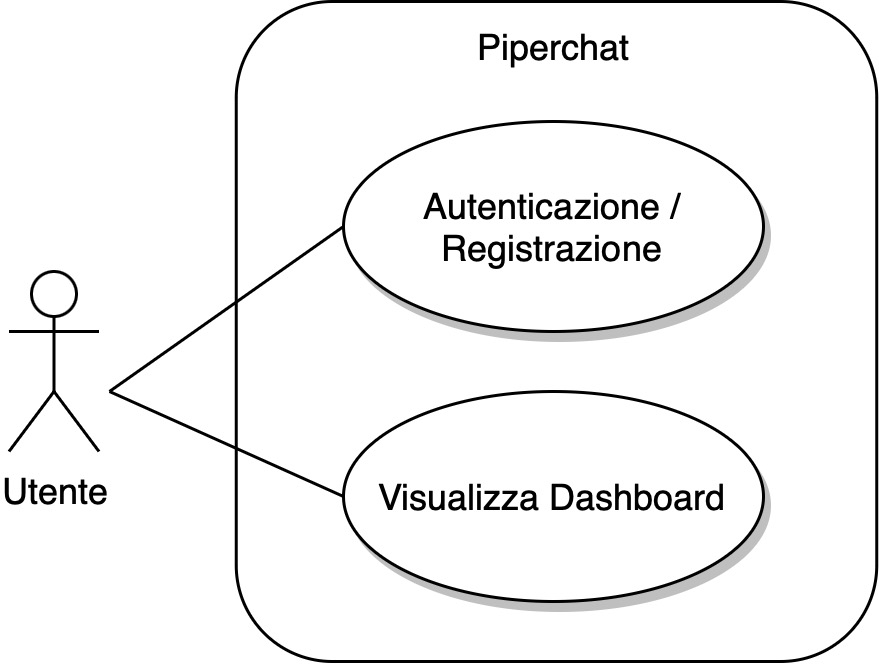
\includegraphics[width=0.6\linewidth]{sections/01-goal/img/use-cases/piperchat-Casi d'uso-1.jpg}
    \caption{Diagramma dei casi d'uso di un utente non autenticato}
\end{figure}

%
%
%
\subsubsection{Utente autenticato}

Dopo aver eseguito l'autenticazione, un utente acquisisce la possibilità di svolgere numerose azione, che riguardano diversi ambiti.
%
Si possono identificare i seguenti scenari:

\begin{enumerate}
    \item L'utente ha ora possibilità di gestire il proprio profilo ed è abilitato a ricevere le notifiche a lui indirizzate.

    \item L'utente può utilizzare la gestione delle richieste di amicizia che prevede di poter 
        \begin{enumerate*}
            \item inviarne ad altri utenti,
            \item accettare le richieste ricevute
            \item rifiutare le richieste ricevute.
        \end{enumerate*}
        
    \item L'utente ha la possibilità di creare server oppure partecipare a server già creati.
\end{enumerate}

\begin{figure}[H]
    \centering
    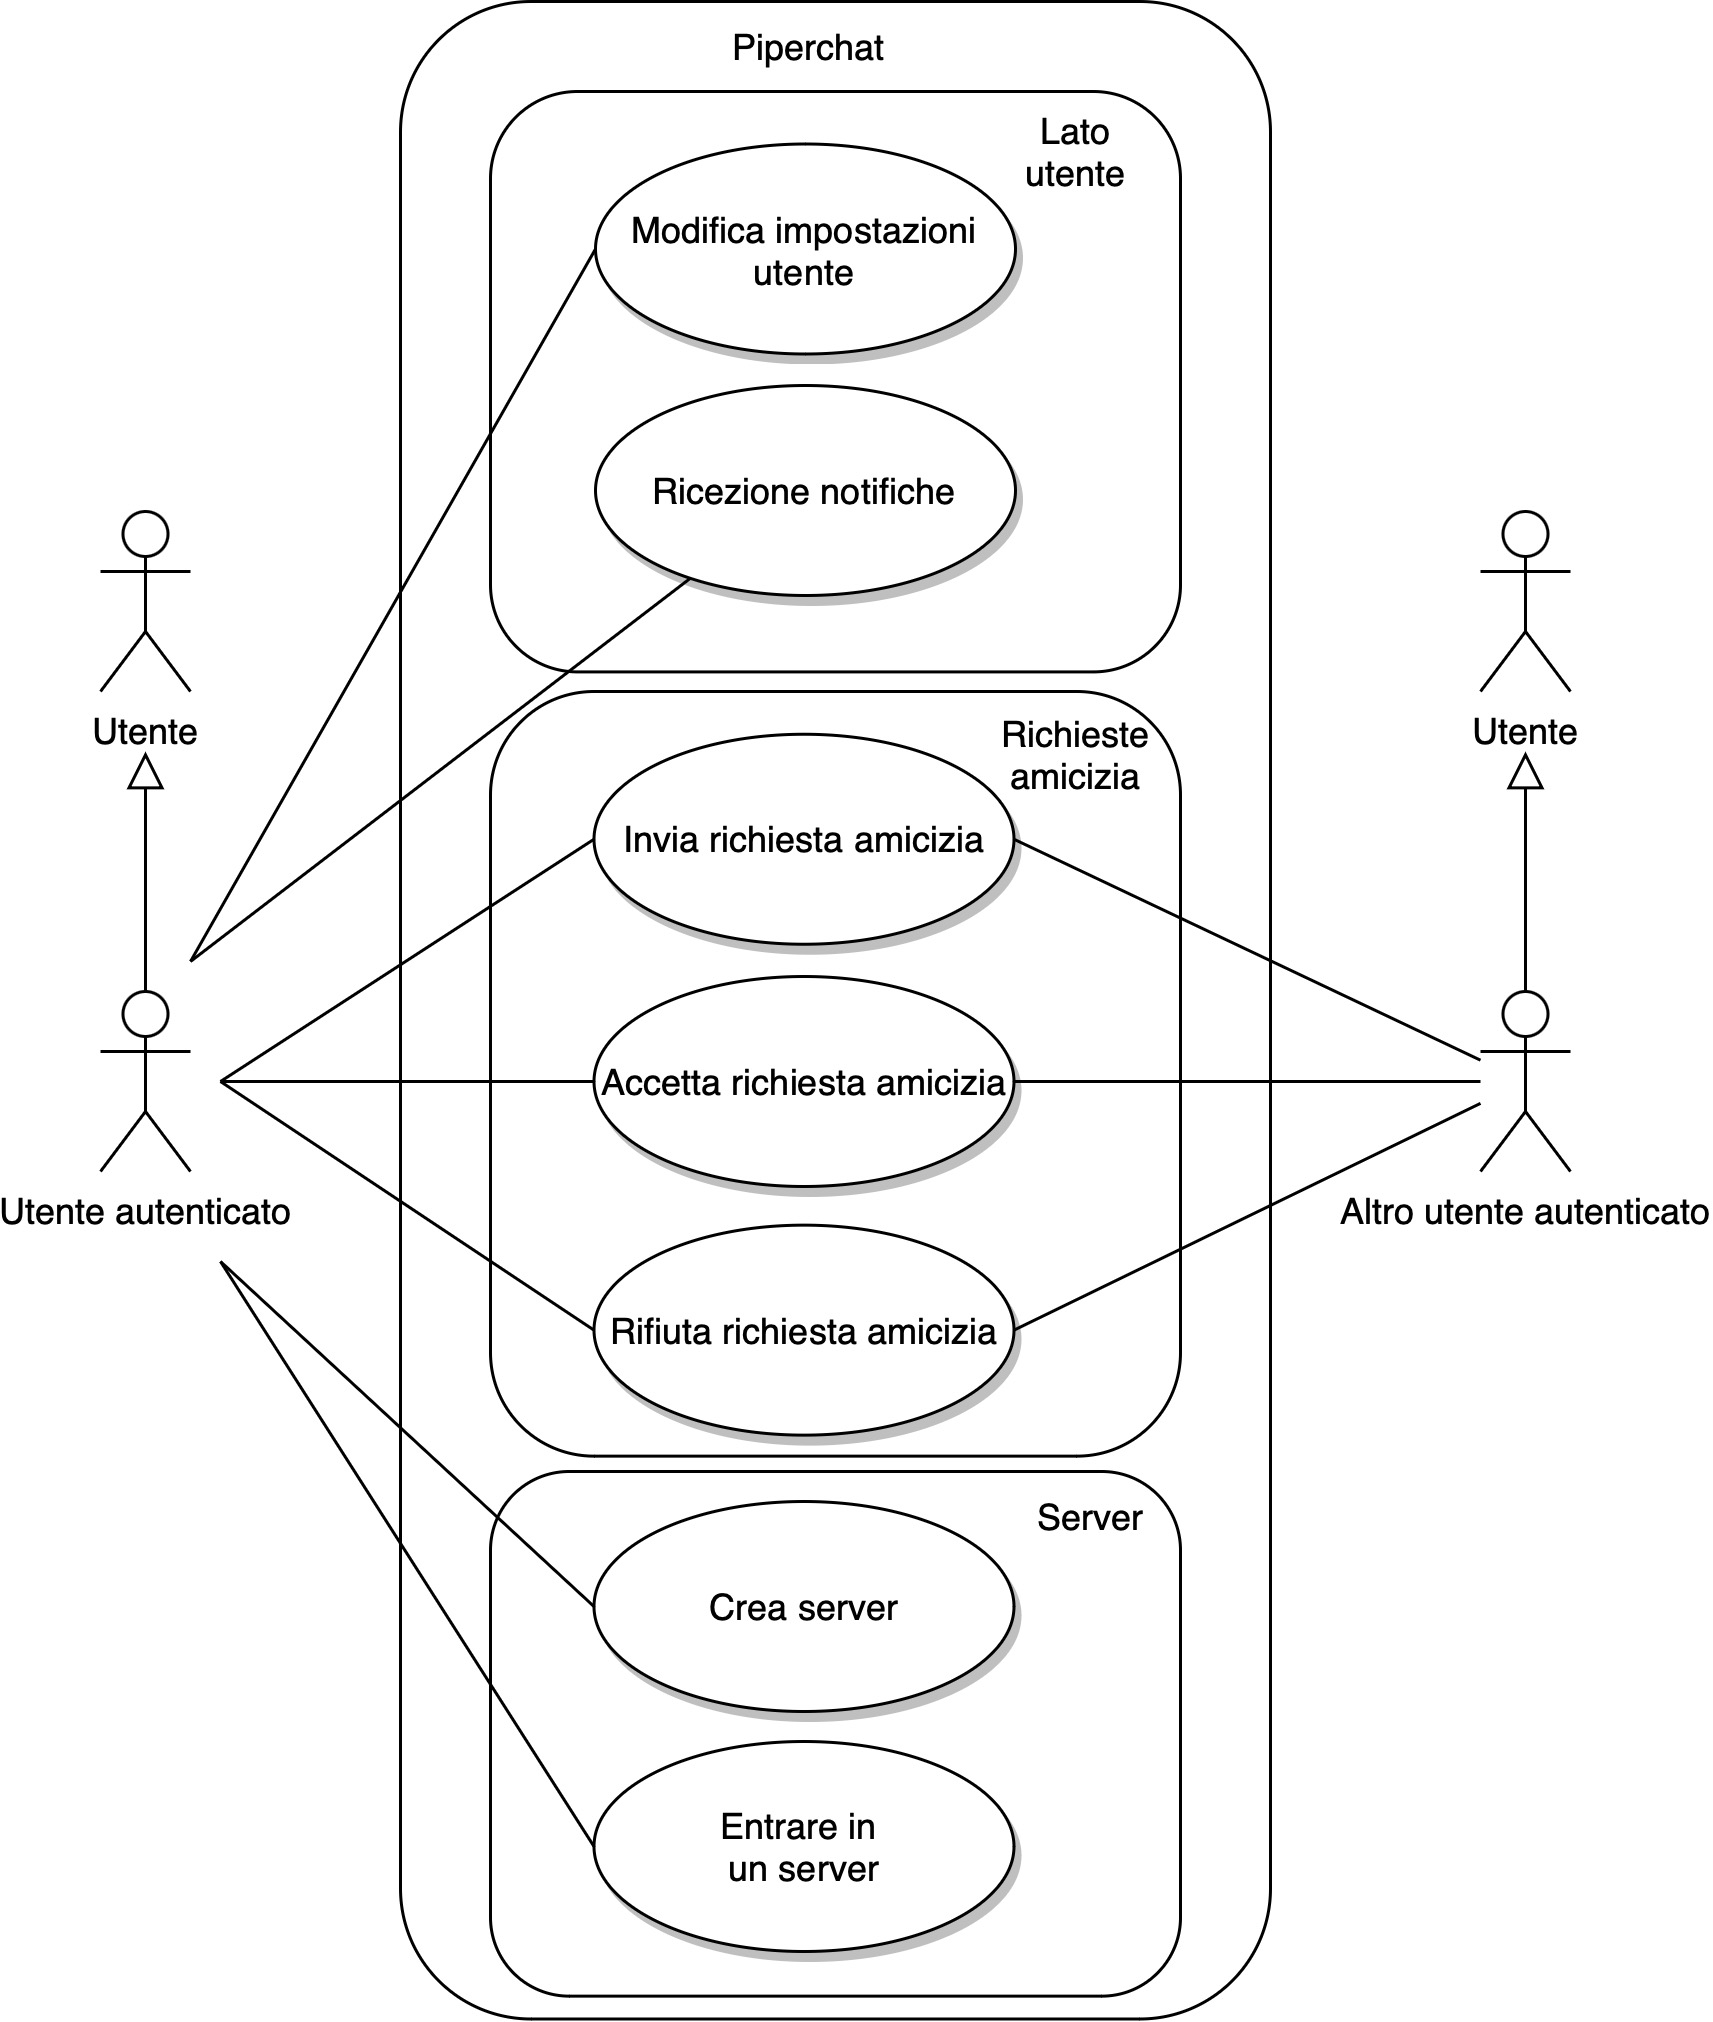
\includegraphics[width=1\linewidth]{sections/01-goal/img/use-cases/piperchat-Casi d'uso-2.jpg}
    \caption{Diagramma dei casi d'uso di un utente autenticato}
\end{figure}

%
%
%
\subsubsection{Utente amministratore di server}

Un utente, dopo aver creato un server, ne diventa amministratore.
%
Questo permette di accedere alle funzionalità di gestione per esso, tra le quali si possono evidenziare le seguenti:

\begin{enumerate}
    \item L'amministratore può aggiornare le informazioni del server o eliminarlo.

    \item L'amministratore può rimuovere un utente dal server.

    \item L'amministratore può creare i canali (testuali o multimediali).

    \item L'amministratore può aggiornare o rimuovere i canali già creati.
\end{enumerate}

\begin{figure}[H]
    \centering
    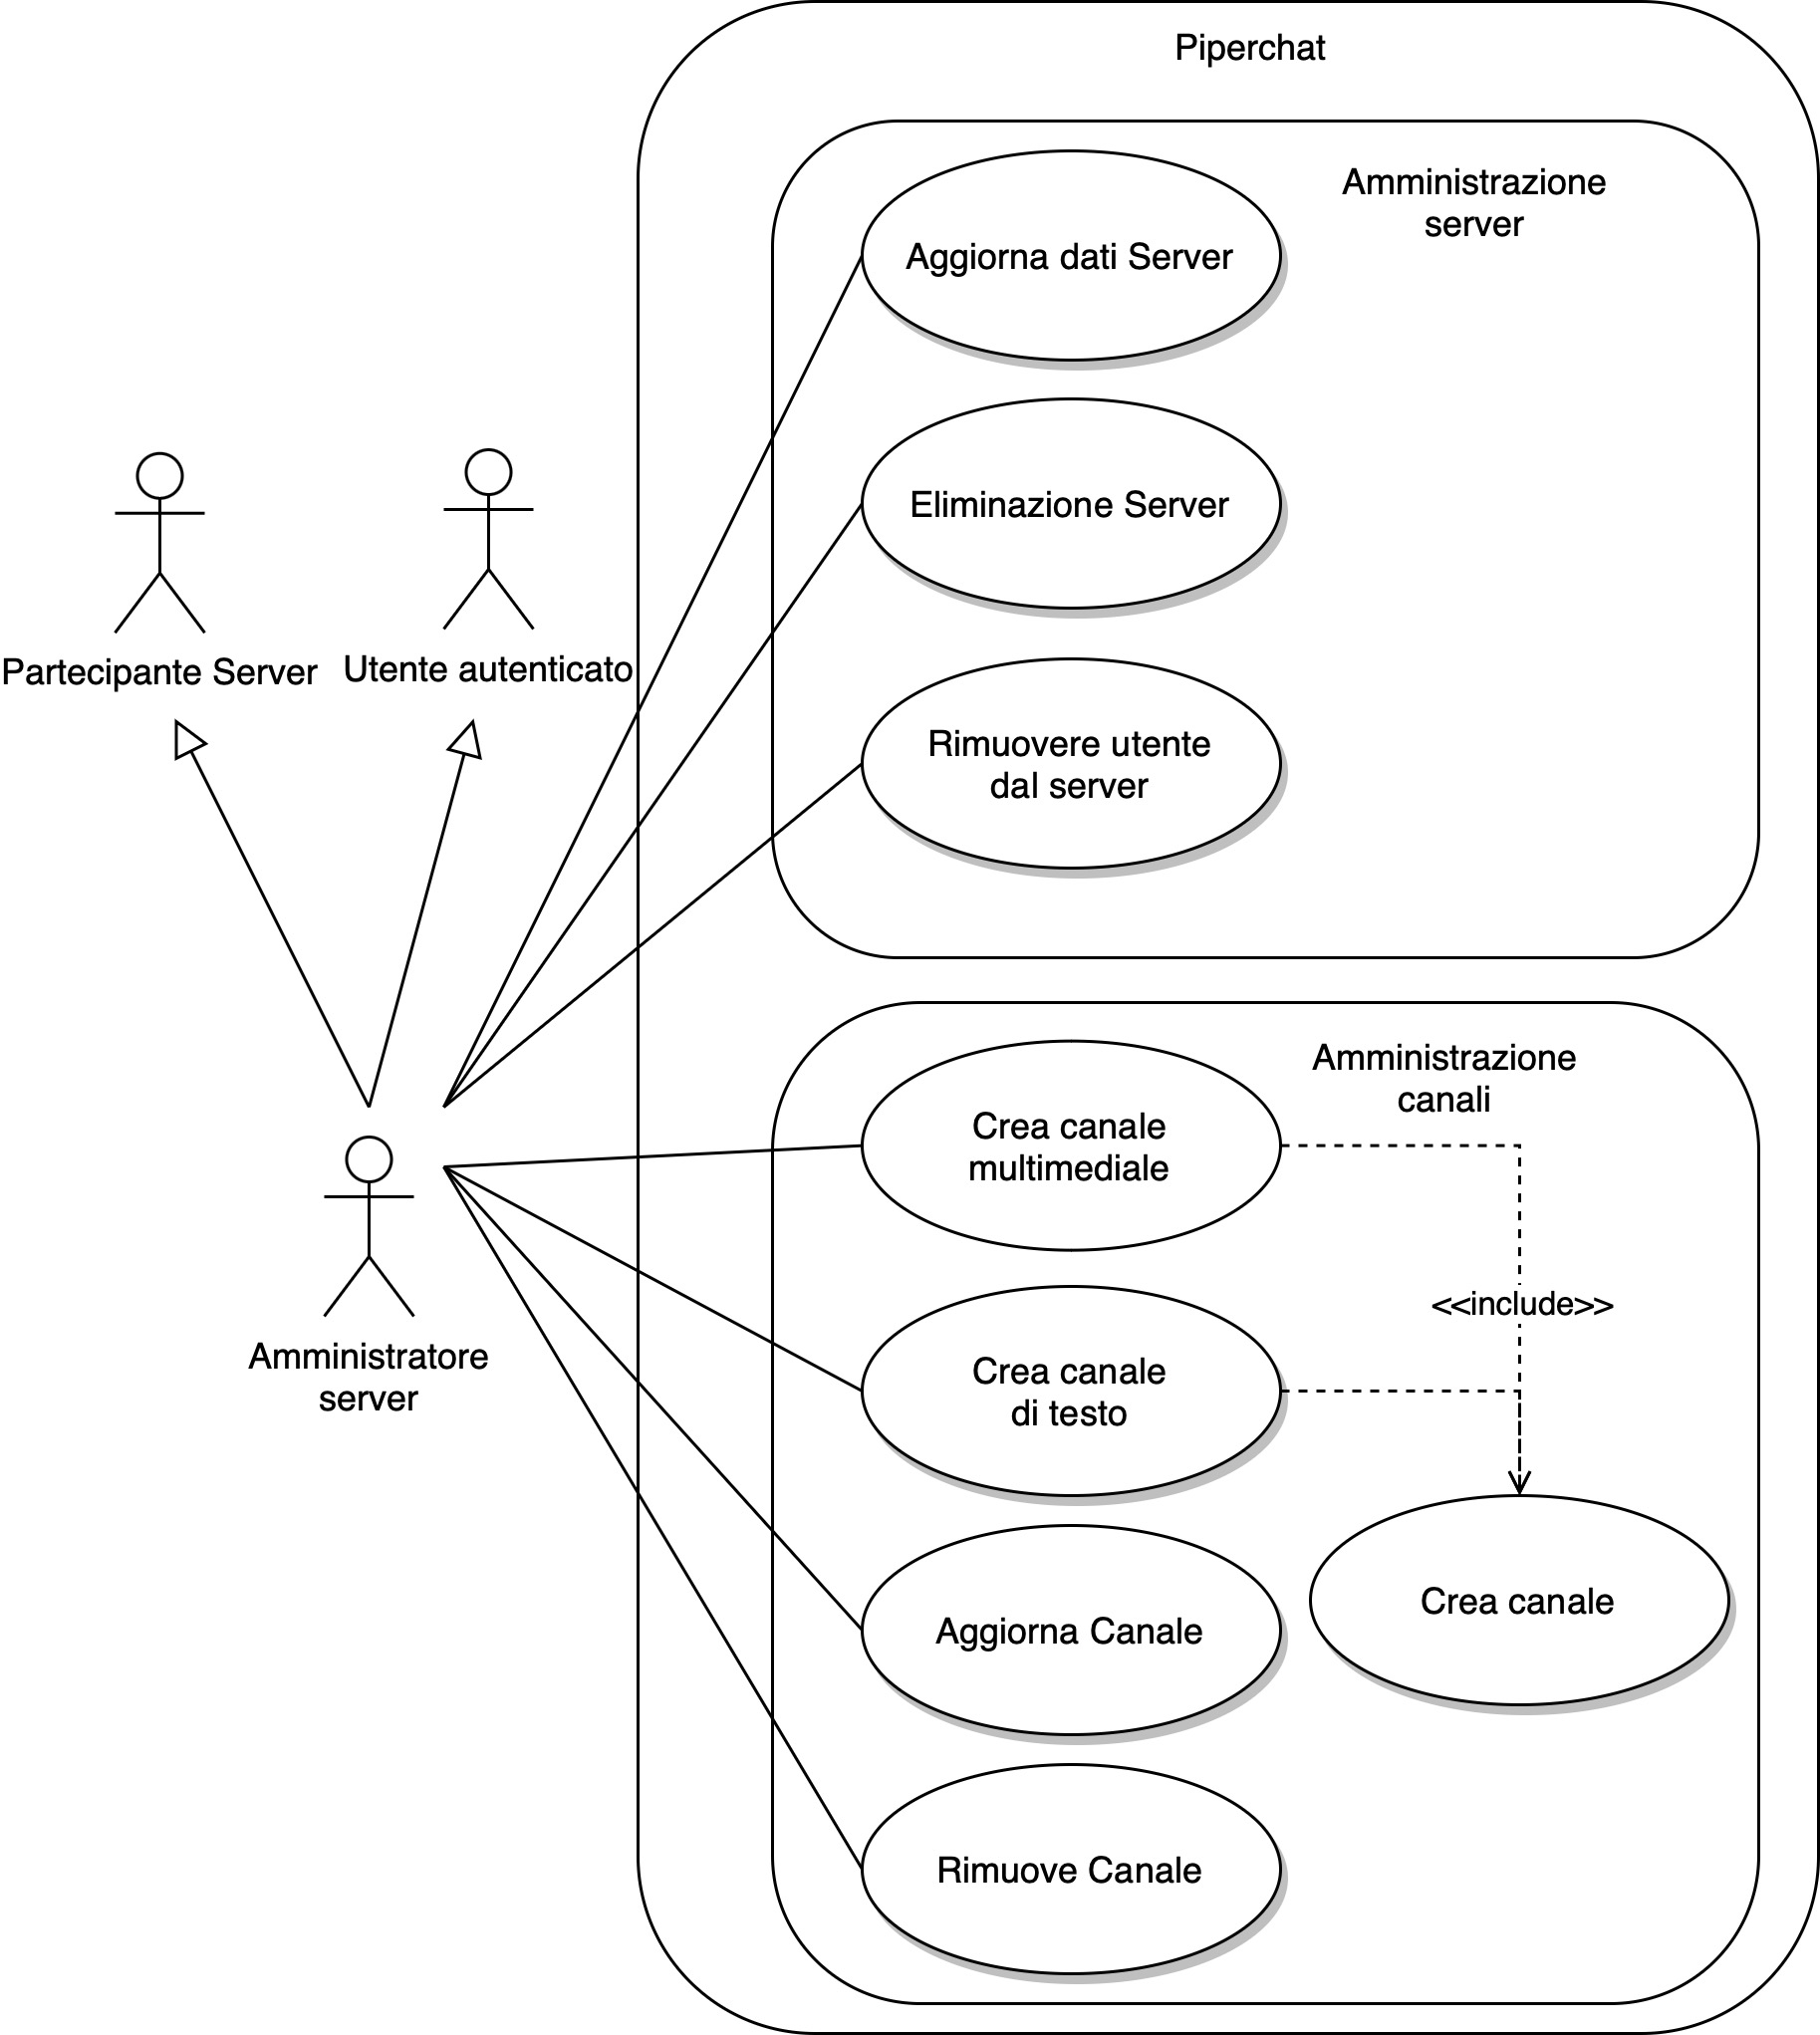
\includegraphics[width=1\linewidth]{sections/01-goal/img/use-cases/piperchat-Casi d'uso-3.jpg}
    \caption{Diagramma dei casi d'uso di un utente amministrazione di un server}
\end{figure}

%
%
%
\subsubsection{Interazione tra utente e amici}

Due utenti, dopo aver stretto amicizia, hanno la possibilità di interagire fra loro nei seguenti modi:

\begin{enumerate}
    \item Inviare messaggi all'interno della chat tra i due utenti.

    \item Partecipare alla sessione multimediale.
\end{enumerate}

\begin{figure}[H]
    \centering
    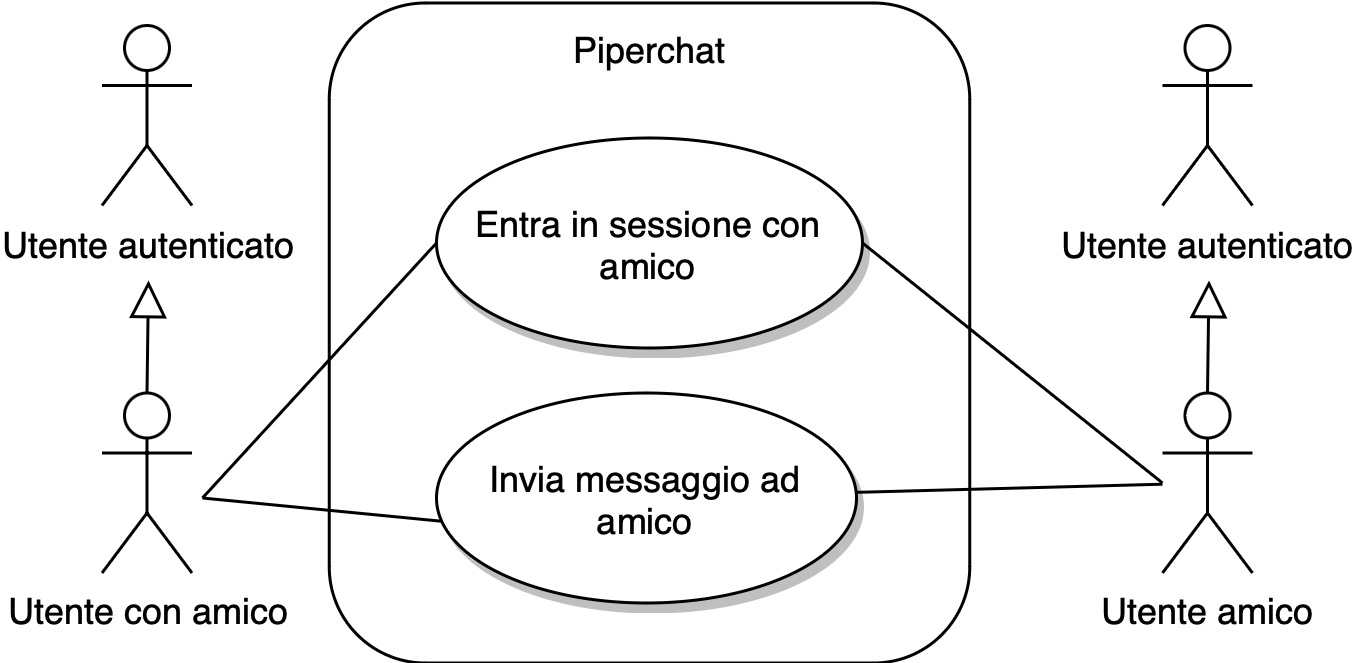
\includegraphics[width=1\linewidth]{sections/01-goal/img/use-cases/piperchat-Casi d'uso-4.jpg}
    \caption{Diagramma dei casi d'uso di un utente che interagisce con un amico}
\end{figure}

%
%
%
\subsubsection{Interazione di un utente partecipante ad un server}

Un utente che partecipa ad un server ha la possibilità di interazione attraverso i canali che sono stati creati, nei quali può:

\begin{enumerate}
    \item Inviare messaggi all'interno dei canali testuali.

    \item Partecipare ad un sessione in un canale multimediale.
\end{enumerate}

\begin{figure}[H]
    \centering
    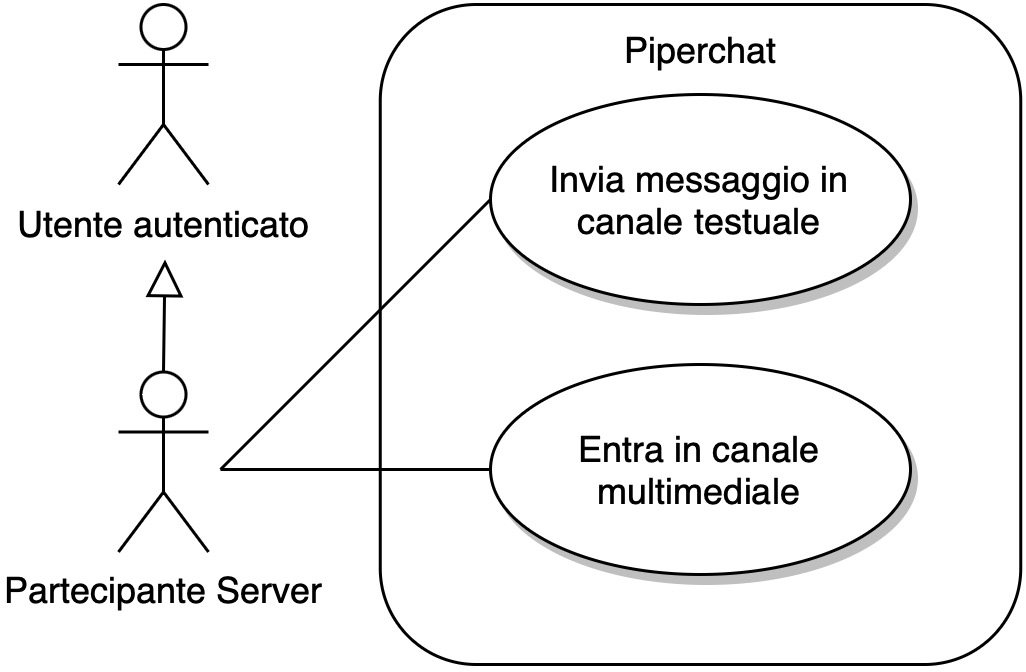
\includegraphics[width=0.6\linewidth]{sections/01-goal/img/use-cases/piperchat-Casi d'uso-5.jpg}
    \caption{Diagramma dei casi d'uso di un utente che partecipa ad un server}
\end{figure}

%
%
%
\subsubsection{Utente in sessione multimediale}

Un utente in sessione multimediale, sia in una privata con un amico, che in un canale, ha la possibilità di gestire microfono e webcam e di uscire dalla sessione stessa.

\begin{figure}[H]
    \centering
    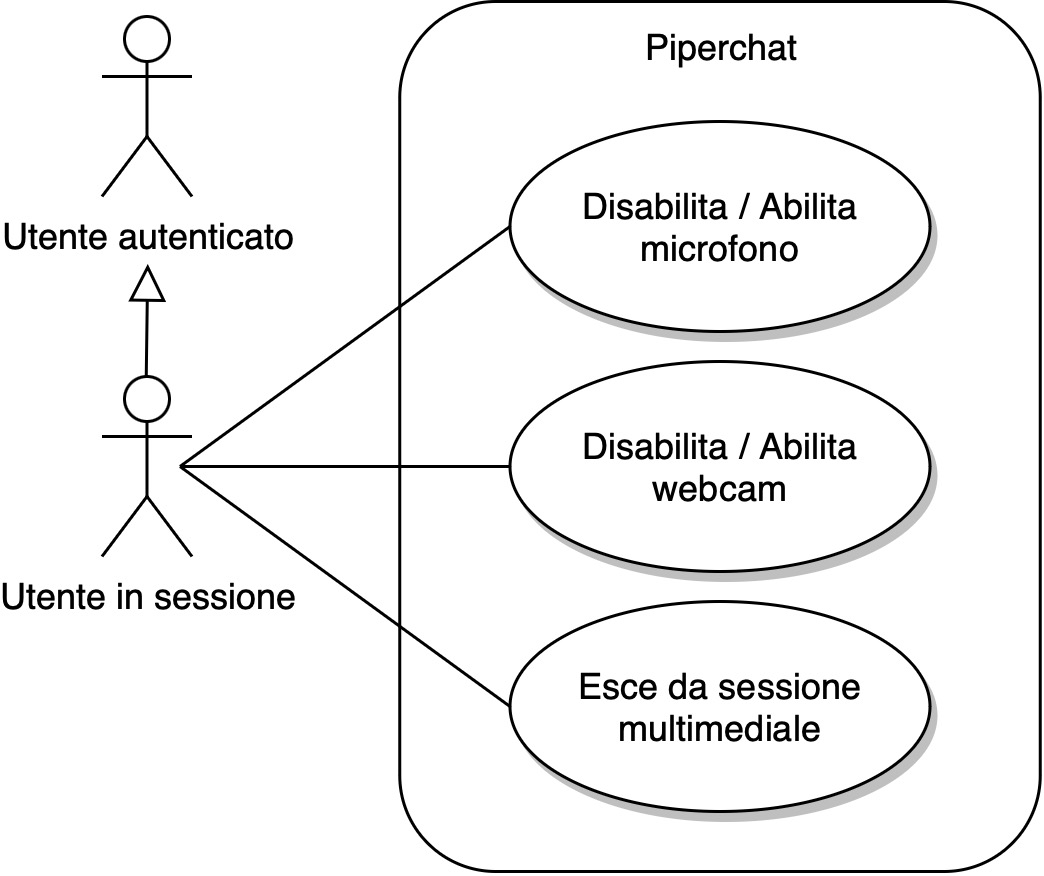
\includegraphics[width=0.7\linewidth]{sections/01-goal/img/use-cases/piperchat-Casi d'uso-6.jpg}
    \caption{Diagramma dei casi d'uso di un utente che partecipa ad una sessione}
\end{figure}

% \begin{figure}[H]
%     \centering
%     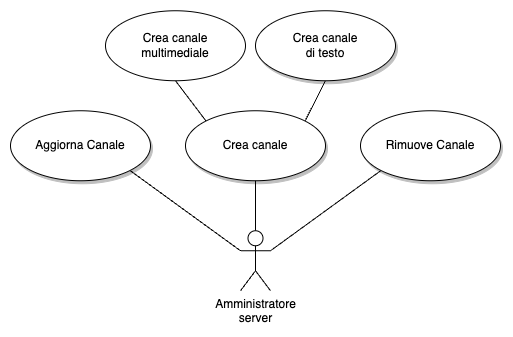
\includegraphics[width=0.7\linewidth]{sections/01-goal/img/use-cases/piperchat-Casi d'uso-9.drawio.png}
%     \caption{Caso d'uso di un utente amministratore di un server}
% \end{figure}

% \begin{figure}[H]
%     \centering
%     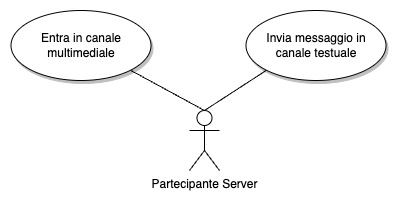
\includegraphics[width=0.7\linewidth]{sections/01-goal/img/use-cases/piperchat-Casi d'uso-10.drawio.png}
%     \caption{Caso d'uso di un utente partecipante di un server}
% \end{figure}

% \begin{figure}[H]
%     \centering
%     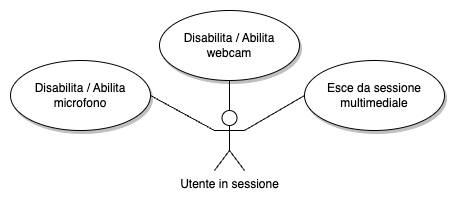
\includegraphics[width=0.7\linewidth]{sections/01-goal/img/use-cases/piperchat-Casi d'uso-6.drawio.png}
%     \caption{Caso d'uso di un utente in una sessione multimediale}
% \end{figure}

%
%
%
\subsection{Politica di autovalutazione}

%\begin{itemize}
%    \item How should the \emph{quality} of the %\emph{produced software} be assessed?
%    
%    \item How should the \emph{effectiveness} of the project %outcomes be assessed?
%\end{itemize}

Nella valutazione della \emph{qualità} del \emph{software prodotto} per il progetto \textit{PiperChat}, verrà adottato un approccio che tiene in considerazione i seguenti fattori:

\begin{itemize}
    \item \textbf{Funzionalità:} Le funzionalità principali del software, inclusi l'autenticazione degli utenti, la gestione delle amicizie, la messaggistica, la creazione di server e le funzionalità dei canali, devono essere implementate ed efficaci.

    \item \textbf{Affidabilità:} si valuterà la stabilità e l'affidabilità dell'architettura a microservizi, garantendo una comunicazione e un'interazione senza intoppi tra i diversi componenti.

    \item \textbf{Scalabilità:} 
    %la capacità del sistema di gestire una base utenti in crescita e un'attività crescente sarà un elemento chiave. 
    verrà valutato se l'applicazione avrà la capacità di gestire l'aumentare del carico computazionale legato all'aumentare degli utenti, le interazioni degli stessi, server e canali. Si terrà in considerazione la possibilità di scalabilità orizzontale indipendente del singolo microservizio in modo da consentire una gestione efficiente delle risorse.
    %e una risposta flessibile alle variazioni di carico mirate.

    \item \textbf{Sicurezza:} per quanto concerne gli aspetti di sicurezza, renderemo necessaria l'autenticazione nelle richieste, per garantire la riservatezza e l'integrità delle informazioni degli utenti.

\end{itemize}

Per valutare l'\emph{efficacia} degli esiti del progetto, verranno considerati i seguenti criteri:

\begin{itemize}

    \item \textbf{Decomposizione efficace:} verrà verificata la corretta decomposizione delle funzionalità in microservizi, garantendo che ciascun servizio abbia un ambito ben definito e che le interazioni tra i microservizi siano gestite in modo consono.

    \item \textbf{Dipendenze minime tra Microservizi:} si cercherà di minimizzare le dipendenze tra i microservizi, favorendo l'indipendenza e la modularità per semplificare la gestione e favorire la manutenibilità.

    \item \textbf{Reattività agli Eventi:} verrà assicurata una risposta pronta agli eventi attraverso l'implementazione di meccanismi di \emph{event-driven architecture} tra i microservizi e verso gli utenti finali.

    % \item \textbf{Scalabilità Indipendente:} si valuterà la capacità di ciascun microservizio di scalare indipendentemente dagli altri, consentendo una gestione efficiente delle risorse e una risposta flessibile alle variazioni di carico mirate.

    \item \textbf{Monitoraggio:} verrà implementato un sistema robusto di monitoraggio per i microservizi, permettendo di osservare l'attuale stato dei microservizi in gioco.
    
    %una rapida individuazione e risoluzione dei problemi, nonché una comprensione dettagliata delle attività del sistema.

\end{itemize}

% \section{Expected work plan}

Is there any implicit requirement hidden within this project's requirements?
%
Is there any implicit hypothesis hidden within this project's requirements?
%
Are there any non-functional requirements implied by this project's requirements?

What model / paradigm / techonology is the best suited to face this project's requirements?
%
What's the abstraction gap among the available models / paradigms / techonologies and the problem to be solved?

Lo sviluppo del progetto sarà guidato dalla seguente scaletta, in modo da rendere l'integrazione delle features incrementali.

\begin{enumerate}

    \item Sviluppo scheletro infrastruttura a micro-servizi.
    \begin{enumerate}
        \item Selezione e integrazione del Broker.
        \item Sviluppo sistema Logging per il monitoraggio degli eventi del sistema (utile per monitorare l'incremento delle features)
        \item Sviluppo dashboard reattiva per la visualizzazione dello stato dei servizi.
    \end{enumerate}
    
    \item Sviluppo sistema di utenti.
    \begin{enumerate}
        \item Sistema di registrazione.
        \item Sistema di login
        \item Sistema di gestione stato (online, offline, ultimo accesso, etc..)
    \end{enumerate}

    \item Sviluppo sistema di notifiche
    \begin{enumerate}
        \item Sistema di collegamento tramite websockets.
        \item Sistema di memorizzazione di ricezione delle notifiche.
    \end{enumerate}

    \item Sviluppo sistema di messaggistica intra-utenti
    \begin{enumerate}
        \item Sistema di richieste di amicizia.
        \item Aggiunta supporto notifiche richieste amicizia.
        \item Sistema chat private tra utenti.
        \item Aggiunta supporto notifiche messaggi.
    \end{enumerate}

    \item Sviluppo sistema di gestione dei server.
    \begin{enumerate}
        \item Sistema di creazione server.
        \item Sistema di join dei server.
        \item Sistema di creazione canali testuali all'interno dei server.
    \end{enumerate}

    \item Estensione della messaggistica all'audio/video.
    \begin{enumerate}
        \item Sistema di signaling WebRTC per inizializzazione chiamate.
        \item Sistema di creazione di canali multimediali.
        \item Sistema di chiamate multimediali intra-utenti.
        \item Aggiunta supporto notifiche chiamate in entrata.
    \end{enumerate}

    \item Feature opzionali
    \begin{enumerate}
        \item Sistema di blacklisting intra-utenti.
        \item Sistema di ban degli utenti dai server.
        \item Sviluppo di un servizio adibito al salvataggio dei file inviati dagli utenti in modo da abilitare non solo messaggi testuali ma anche l’invio di file.
        \item Gestione auto-scaling.
    \end{enumerate}

\end{enumerate}

\subsection{Technologies}

Di seguito le tecnologie che verranno utilizzate per l'implementazione del progetto:

\begin{itemize}
    \item Node.js per lo sviluppo dei servizi
    \begin{itemize}
        \item Typescript come linguaggio
        \item Express.js per il server
        \item Socket.io per la comunicazione tramite Websocket
        \item Mongoose per la gestione del database
        \item Amqplib per la connessione al broker
        \item Jest per il testing
    \end{itemize}
    \item MongoDB per i database dei servizi
    \item RabbitMQ come broker
    \item Docker + Docker-Compose per l’infrastruttura
    \item HTTP e Websocket come protocolli di comunicazione con i servizi
    \item HTML, Javascript e CSS per il client Web.
    \item WebRTC per la comunicazione audio/video
\end{itemize}

\chapter{Requisiti}
\section{Funzionali}

\begin{itemize}
    \item \textbf{Registrazione e Autenticazione}:
    \begin{itemize}
        \item Possibilità di registrazione al sistema.
        
        \item Possibilità di login nel sistema.
    \end{itemize}
    \item \textbf{Sistema di amicizie}:
    \begin{itemize}
        \item Possibilità di inviare richieste di amicizia.
        
        \item Possibilità di accettare o rifiutare richieste di amicizia.
        
        \item Sistema di notifiche per la ricezione di nuovo richieste di amicizia.
        
        \item Sistema di gestione dello stato e dell'ultimo accesso degli utenti.
    \end{itemize}
    \item \textbf{Messaggistica Infra-Utente}:
    \begin{itemize}
        \item Gestione messaggistica tra amici
        
        \item Sistema di notifiche per l'arrivo di nuovi messaggi.
    \end{itemize}
    \item \textbf{Gestione Server}:
    \begin{itemize}
        \item Possibilità di creazione di un nuovo server.
        
        \item Possibilità di join di un server esistente.
        
        \item Possibilità da parte del creatore del server di rimozione dei membri.
    \end{itemize}
    \item \textbf{Gestione canali testuali}:
    \begin{itemize}
        \item Possibilità di creazione di canali testuali da parte dell'owner del server.
        \item Possibilità di rimozione di canali testuali da parte dell'owner del server.
        \item Sistema di messaggistica per i canali testuali
        \item Sistema di notifiche per i nuovi messaggi inviati all'interno di canali testuali.
    \end{itemize}
    \item \textbf{Gestione canali multimediali}:
    \begin{itemize}
        \item Possibilità di creazione di canali multimediali da parte dell'owner del server.
        \item Possibilità di rimozione di canali multimediali da parte dell'owner del server.
        \item Sistema di videochiamate.
        \item Gestione della webcam e del microfono.
    \end{itemize}
\end{itemize}

\section{Requisiti non Funzionali (Usabilità e Accessibilità)}
\begin{itemize}
    \item \textbf{Sistema di monitoring dei microservizi}:
    \begin{itemize}
        \item Sistema di monitoraggio dello stato dei servizi.
        \item Dashboard per visualizzare lo stato real-time dei servizi.
    \end{itemize}
    
    \item \textbf{Supporto temi}: l'applicazione deve poter gestire il cambio di tema, offrendo anche un opzione a supporto di utenti con dislessia.
    
    \item \textbf{Test di Accessibilità}: Prima del rilascio ufficiale, l'applicazione deve essere sottoposta a test di accessibilità per identificare e correggere eventuali problemi relativi all'accessibilità.
\end{itemize}



\chapter{Design}

Il progetto è stato guidato da un modello iterativo basato sullo \textbf{User Centered Design}.
%
Inizialmente, sono stati definiti gli utenti target dell'applicazione, sui quali sono state create le \textit{Personas}.
%
Queste ultime hanno svolto un ruolo cruciale nello sviluppo e nella comprensione delle funzionalità del sistema, garantendo un adattamento ai requisiti degli utenti.

Come processo di sviluppo abbiamo adottato una metodologia simile all'Agile, in cui sono state frequentemente analizzate le attività da svolgere e le relative priorità, così come il carico di lavoro assegnato e i feedback sul lavoro svolto.
%
Lato frontend, le interfacce utente sono state progettate secondo i principi fondamentali del design:

\begin{itemize}
    \item il \textbf{KISS} (Keep It Simple, Stupid) per garantire un'esperienza priva di complicazioni e ridurre al minimo gli errori degli utenti durante la navigazione nell'applicazione.
    \item Sono stati impiegati i principi del Responsive Design come base per garantire un elevato livello di usabilità dell'applicazione.
\end{itemize}

%
%
%
\section{Target User Analisys}

Nel processo di progettazione del nostro sistema, abbiamo identificato diversi profili di utenti per comprendere meglio le esigenze e i comportamenti dei potenziali fruitori del nostro servizio.

%
%
%
\subsection{Personas 1: Il Gamer}

\textbf{Nome:} Luca

\textbf{Età:} 23

\textbf{Occupazione:} Studente universitario e appassionato di videogiochi

\textbf{Obiettivi e Comportamenti:} Luca è un giocatore accanito che trascorre molte ore al giorno giocando a una varietà di giochi online. Cerca una piattaforma come la nostra per connettersi con altri giocatori, formare squadre e partecipare a sessioni di gioco cooperative. È interessato a funzionalità quali chat vocali durante il gioco, organizzazione di eventi e discussioni sui giochi più popolari. La sua priorità è un'interfaccia semplice e reattiva per facilitare la sua partecipazione e l'organizzazione di eventi di gioco.

%
%
%
\textbf{Personas 2: Elisa - L'appassionata di Lettura e Libri}

\textbf{Età:} 35

\textbf{Occupazione:} Libraia e Blogger

\textbf{Obiettivi e Comportamenti:} Elisa è appassionata di libri e gestisce un blog letterario. Cerca una piattaforma per connettersi con altri lettori, organizzare club del libro online e discutere di opere letterarie. Desidera una piattaforma con chat testuali, possibilità di creare gruppi tematici dedicati ai diversi generi letterari e strumenti per organizzare eventi come letture collettive e sessioni di discussione.

%
%
%
\subsection{Personas 3: Lo Studente Organizzato}

\textbf{Nome:} Giada

\textbf{Età:} 19

\textbf{Occupazione:} Studentessa universitaria

\textbf{Obiettivi e Comportamenti:} Giada è una studente impegnata che cerca un'interfaccia per connettersi con altri studenti, partecipare a discussioni relative ai corsi e organizzare gruppi di studio. Desidera un'esperienza di messaggistica testuale intuitiva e efficiente che le consenta di partecipare attivamente alle conversazioni relative alle sue lezioni e argomenti di studio. La possibilità di effettuare videochiamate per discussioni di gruppo o sessioni di studio è un aspetto cruciale per lei. Un'interfaccia pulita e facile da usare, specialmente su dispositivi mobili, è essenziale per supportare il suo coinvolgimento attivo nell'apprendimento collaborativo.

%
%
%
\subsection{Riflessioni}

La creazione di queste tre diverse personas ci ha permesso di visualizzare in modo più tangibile e realistico i diversi tipi di utenti che potrebbero utilizzare la piattaforma. Questa analisi ci ha guidato nella progettazione di funzionalità e caratteristiche mirate a soddisfare le esigenze specifiche di ciascun tipo di utente identificato.

%
%
%
\section{Mockup}
Durante la fase di design, è stato utilizzato Figma per la realizzazione di una serie di mockup, nei quali abbiamo testato, diverse combinazioni cromatiche, trovando così le più appropiate per la nostra applicazione.
\\
%
Utilizzando i suoi strumenti, abbiamo potuto esaminare e ottimizzare l'impiego degli spazi, valutando le varie disposizioni degli elementi nel design e assicurandoci che l'esperienza dell'utente fosse ottimale in termini di fluidità e accessibilità.

Di seguito riportati i mockup realizzati durante la fase di design:

\begin{figure}[htbp]
    \centering
    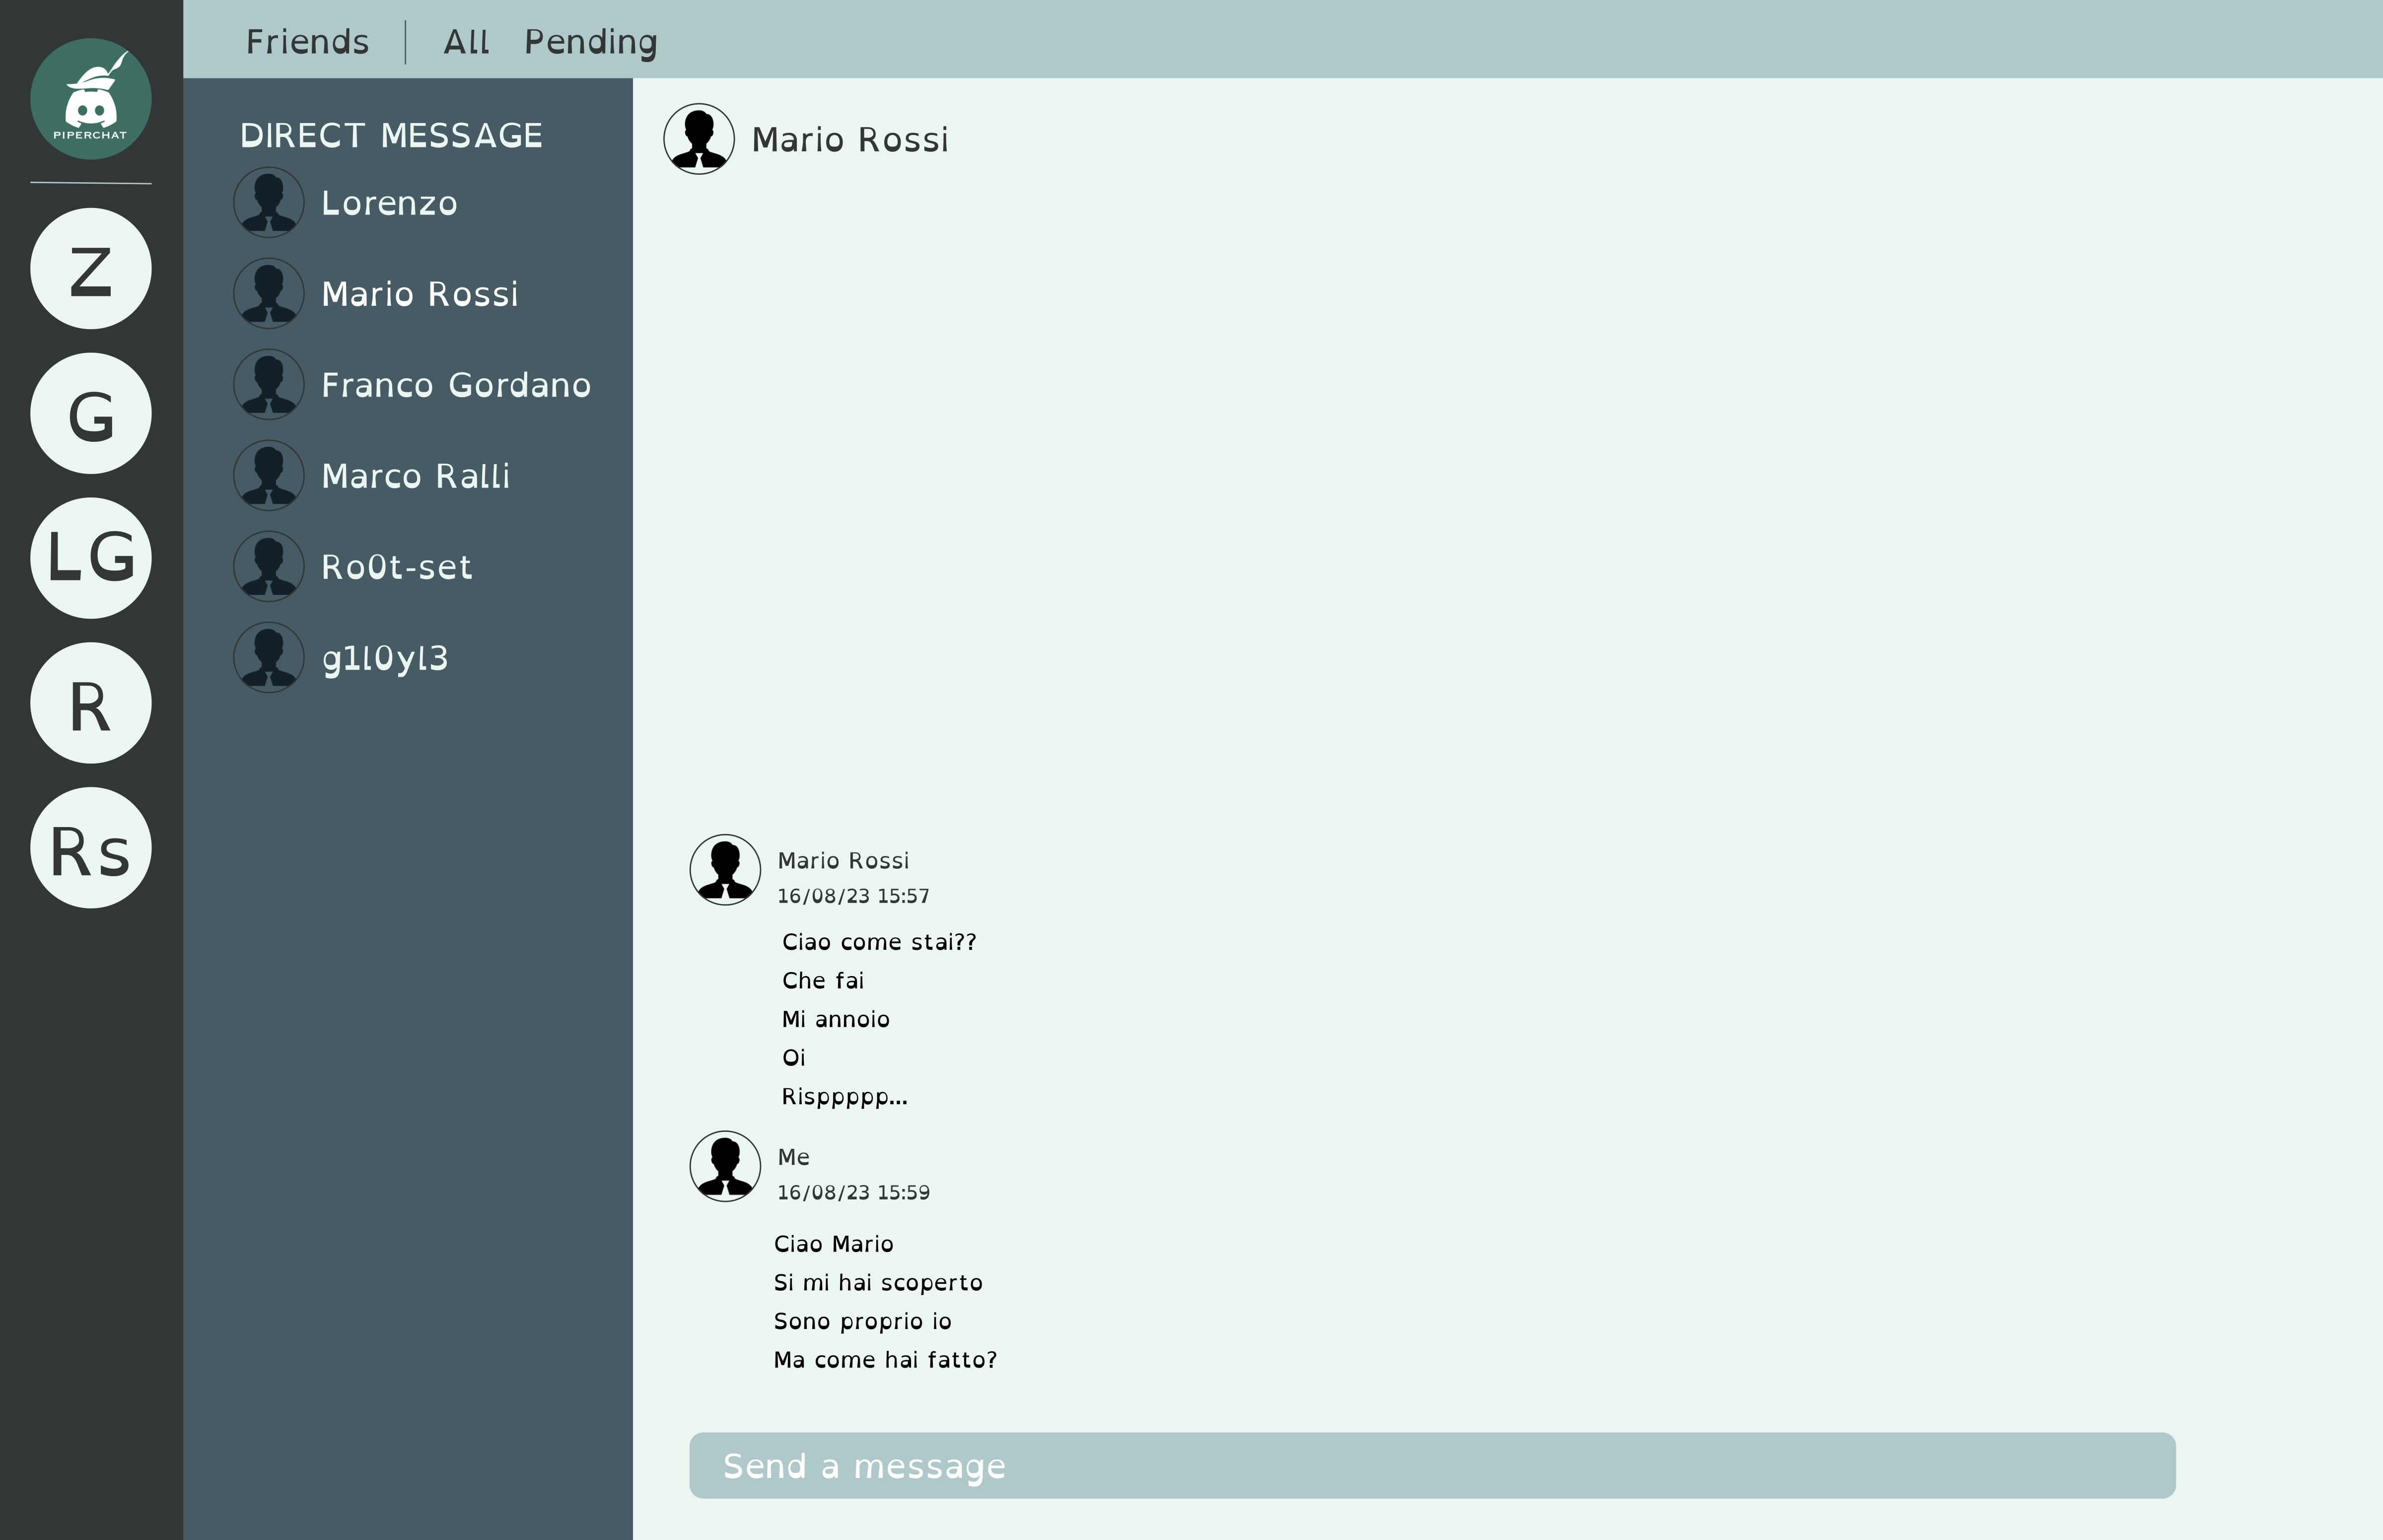
\includegraphics[angle=-90,width=0.92\textwidth]{img/mk2.jpg}
    \caption{Mockup chat}
    \label{fig:mockup2}
\end{figure}

\begin{figure}[htbp]
    \centering
    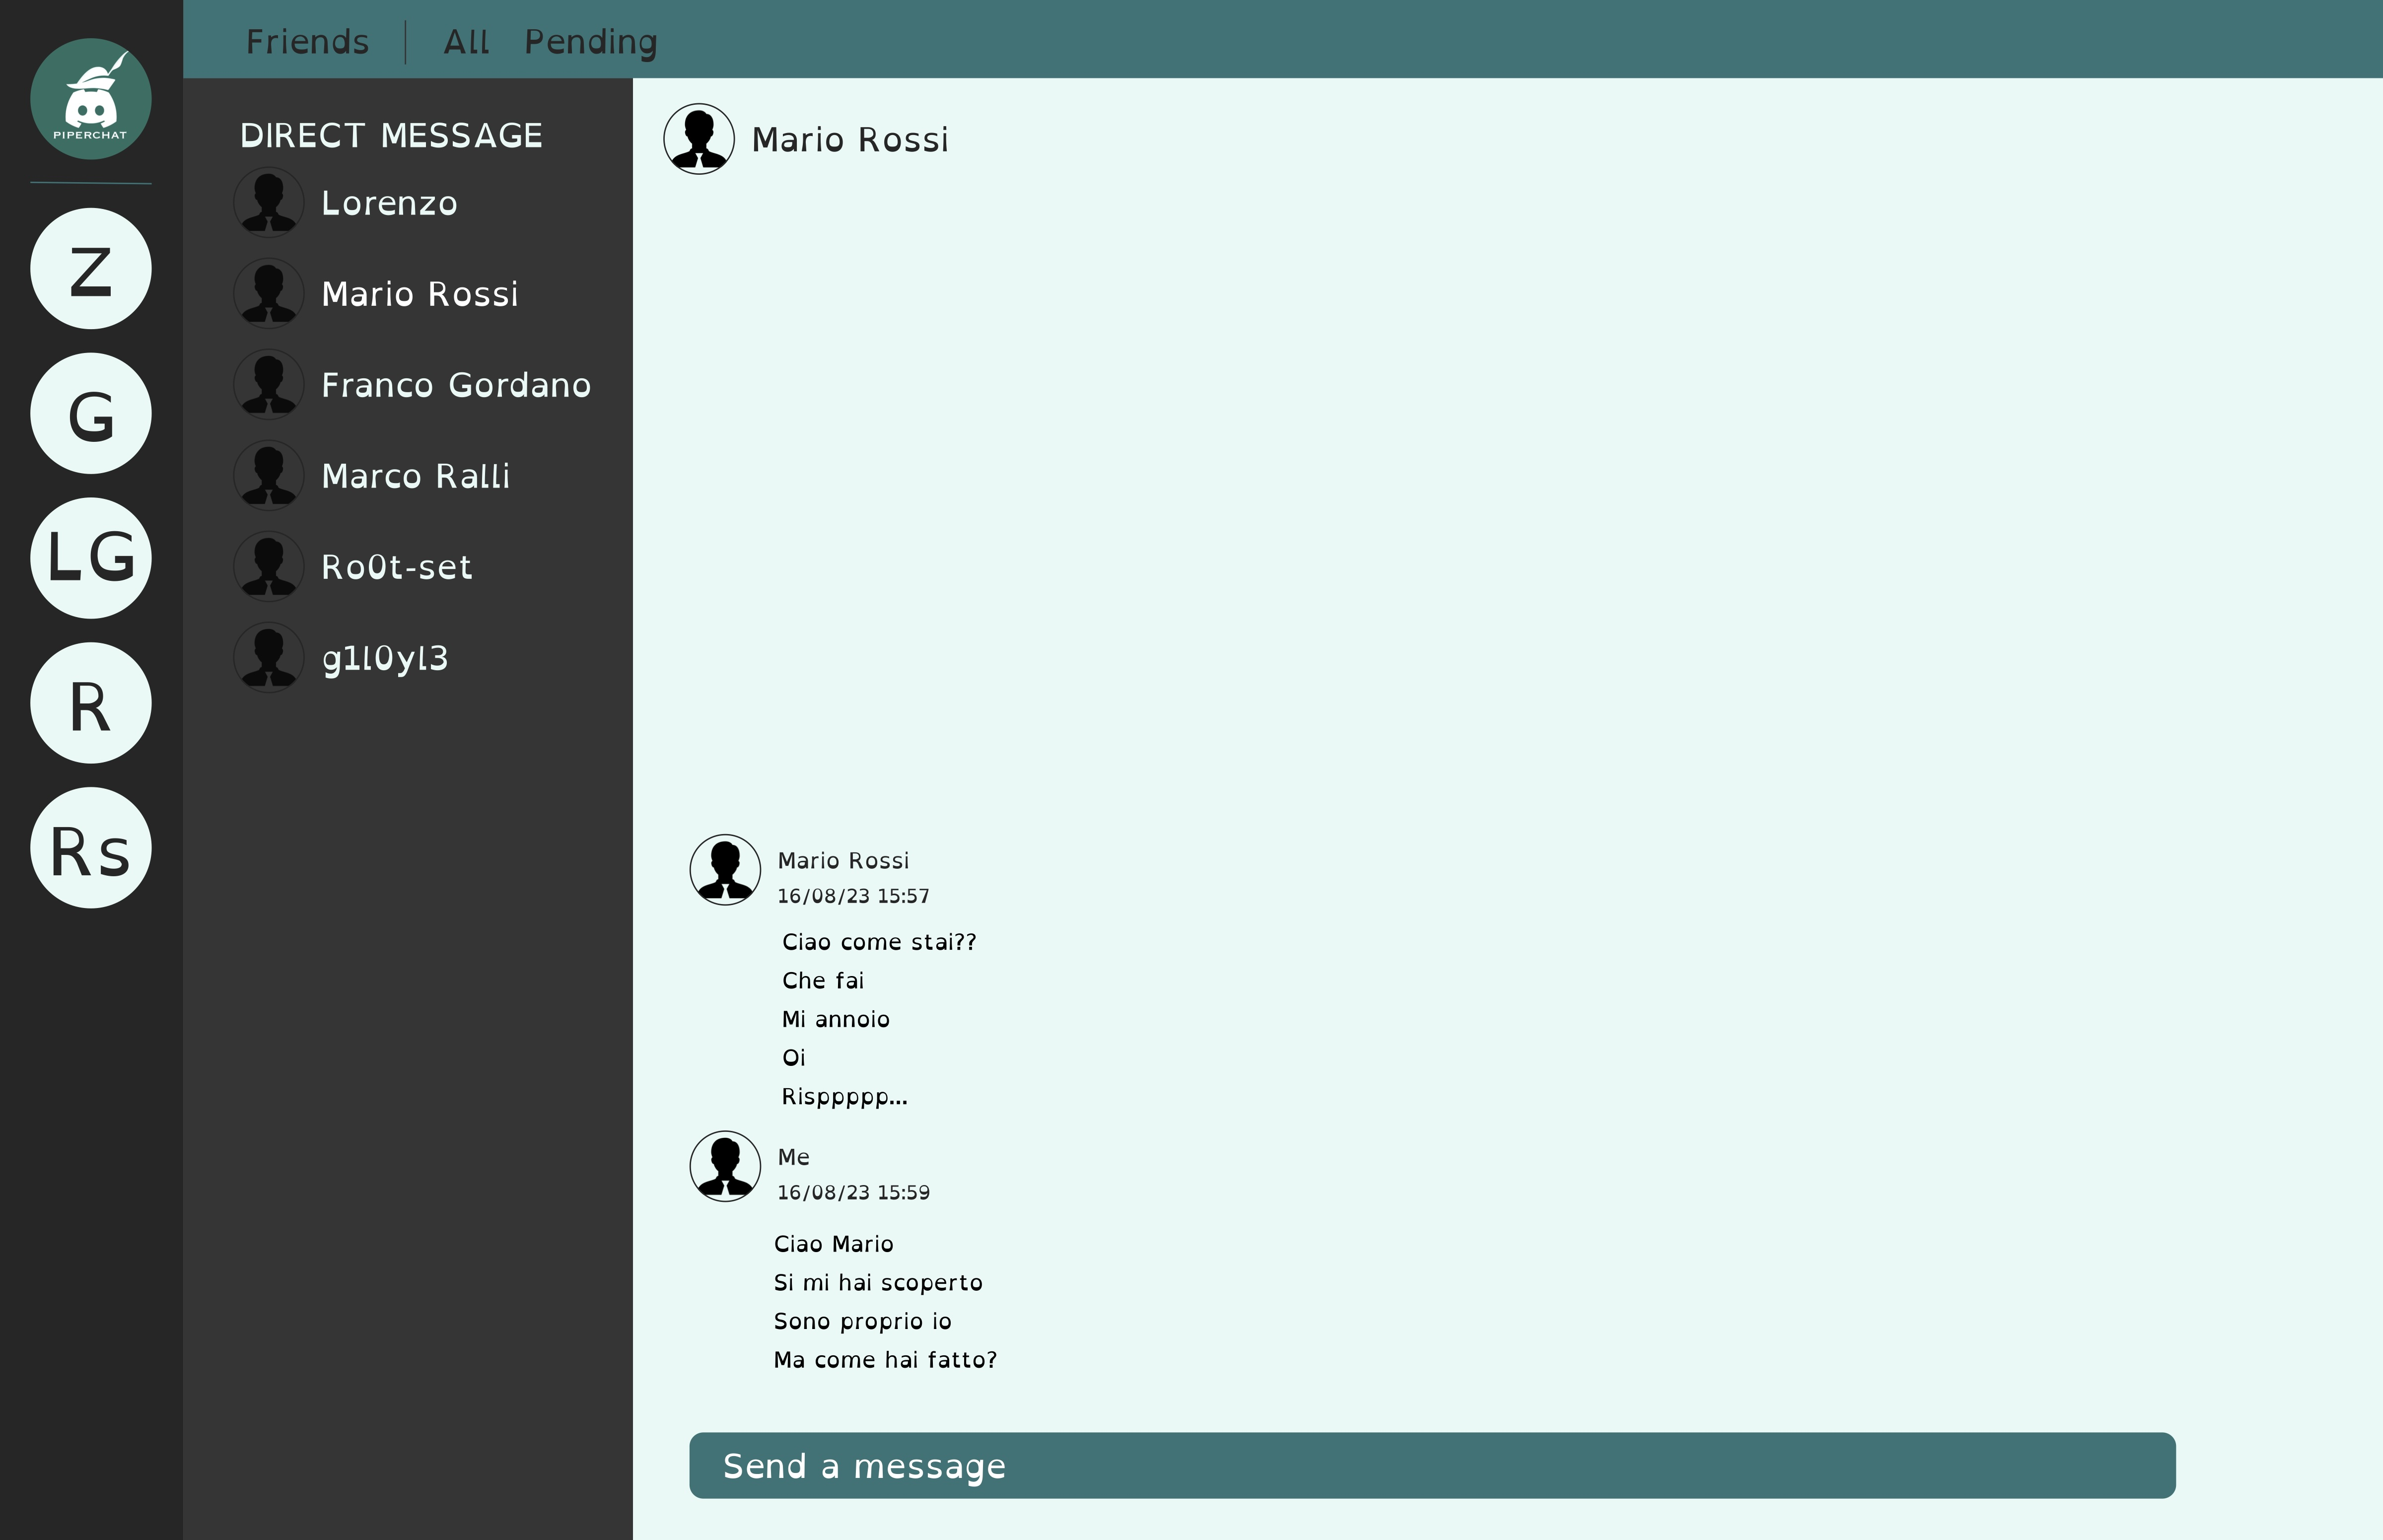
\includegraphics[angle=-90,width=0.92\textwidth]{img/mk3.jpg}
    \caption{Mockup chat con cambio dei colori}
    \label{fig:mockup3}
\end{figure}

\begin{figure}[htbp]
    \centering
    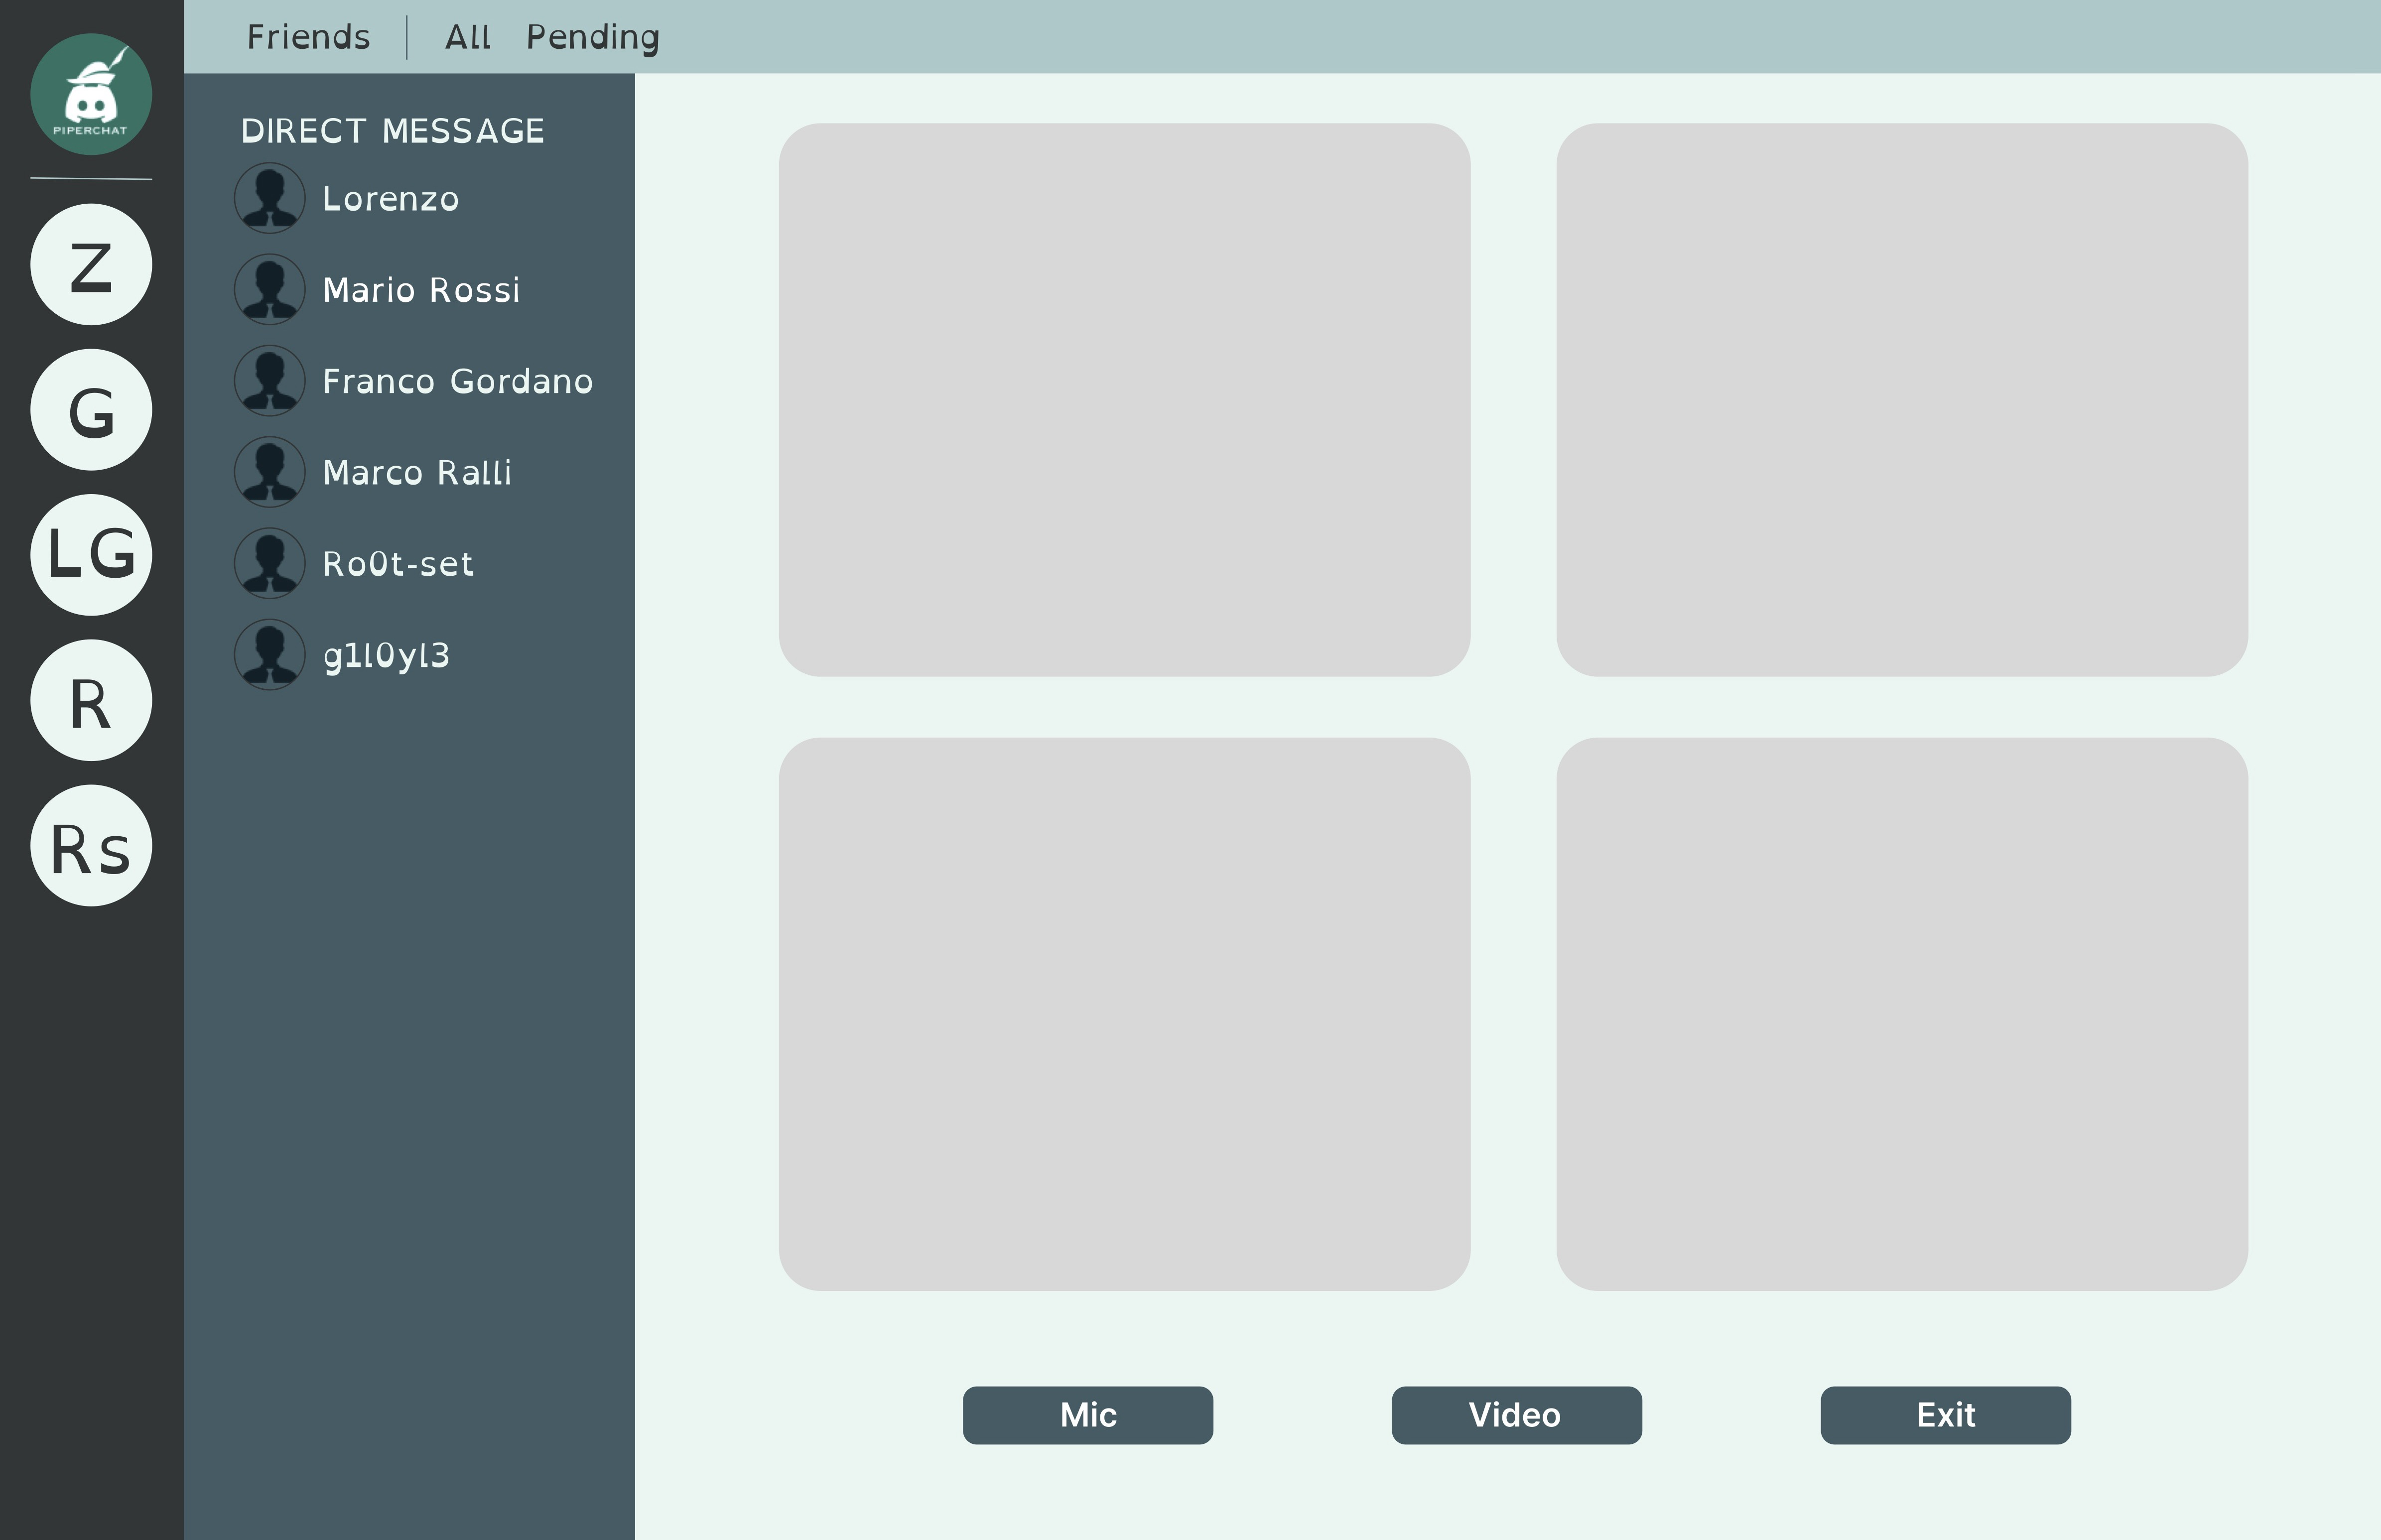
\includegraphics[angle=-90,width=0.92\textwidth]{img/mk4.jpg}
    \caption{Mockup video chat}
    \label{fig:mockup1}
\end{figure}

%
%
%
\newpage
\section{Design Architetturale}

Il sistema è realizzato mediante un'architettura a \emph{microservizi}.
%
Questo permette di suddividere la complessità in parti più piccole, ad alta coesione ed accoppiate in modo lasco.
%
Inoltre, ogni microservizio, se necessario, dispone di un \emph{database}, al quale può accedervi in modo esclusivo.

\begin{figure}[htbp]
    \centering
    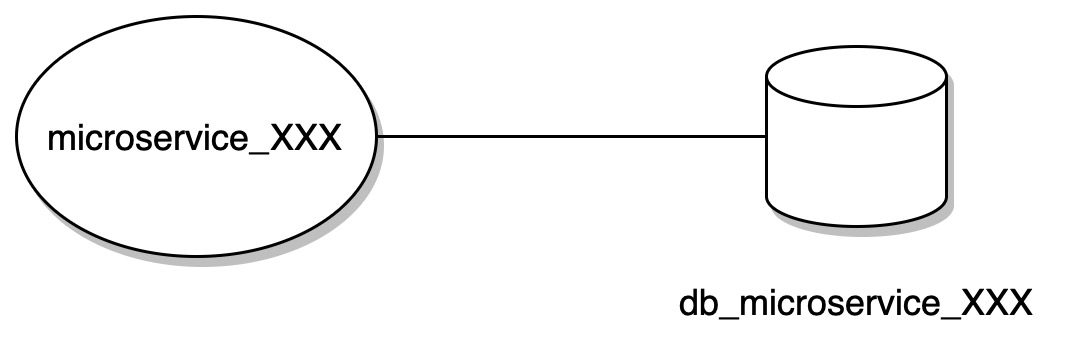
\includegraphics[width=\textwidth]{img/03-design/microservice-db.jpg}
    \caption{Un microservizio con il proprio database}
    \label{fig:microservice-db}
\end{figure}

A fronte di ciò sono stati identificati i seguenti microservizi:

\begin{itemize}
    \item \textbf{Notifications:} permette la gestione delle notifiche e lo status (online, ultimo accesso) degli utenti del sistema;

    \item \textbf{Users:} gestisce l'autenticazione degli utenti al sistema e tutti i dati relativi agli stessi. Inoltre, si occupa delle amicizie fra utenti;

    \item \textbf{Frontend:} fornisce l'accesso al sistema servendo la logica del client come Single Page Application;

    \item \textbf{Messages:} gestisce i messaggi degli utenti, sia nelle chat individuali, che per i canali testuali;

    \item \textbf{Monitoring:} permette il monitoraggio degli altri microservizi;

    \item \textbf{Piperchat:} gestisce la struttura di server e canali del sistema;

    \item \textbf{Webrtc:} gestisce tutto ciò che concerne \emph{WebRTC}, permettendo di istanziare video-chiamate all'interno del sistema.
\end{itemize}

%
%
%
\subsection{Comunicazione}

Al fine di permettere la comunicazione dei microservizi all'interno del sistema e permettere un'interazione con l'esterno, sono identificati i seguenti componenti:

\begin{itemize}
    \item \textbf{API Gateway:} componente che permette la comunicazione tra i client esterni al sistema, con i microservizi. Si occupa di redirezionare le richieste agli appositi servizi.

    \item \textbf{Broker:} componente che permette la comunicazione interna al sistema, fra i microservizi stessi.
\end{itemize}

\begin{figure}[htbp]
    \centering
    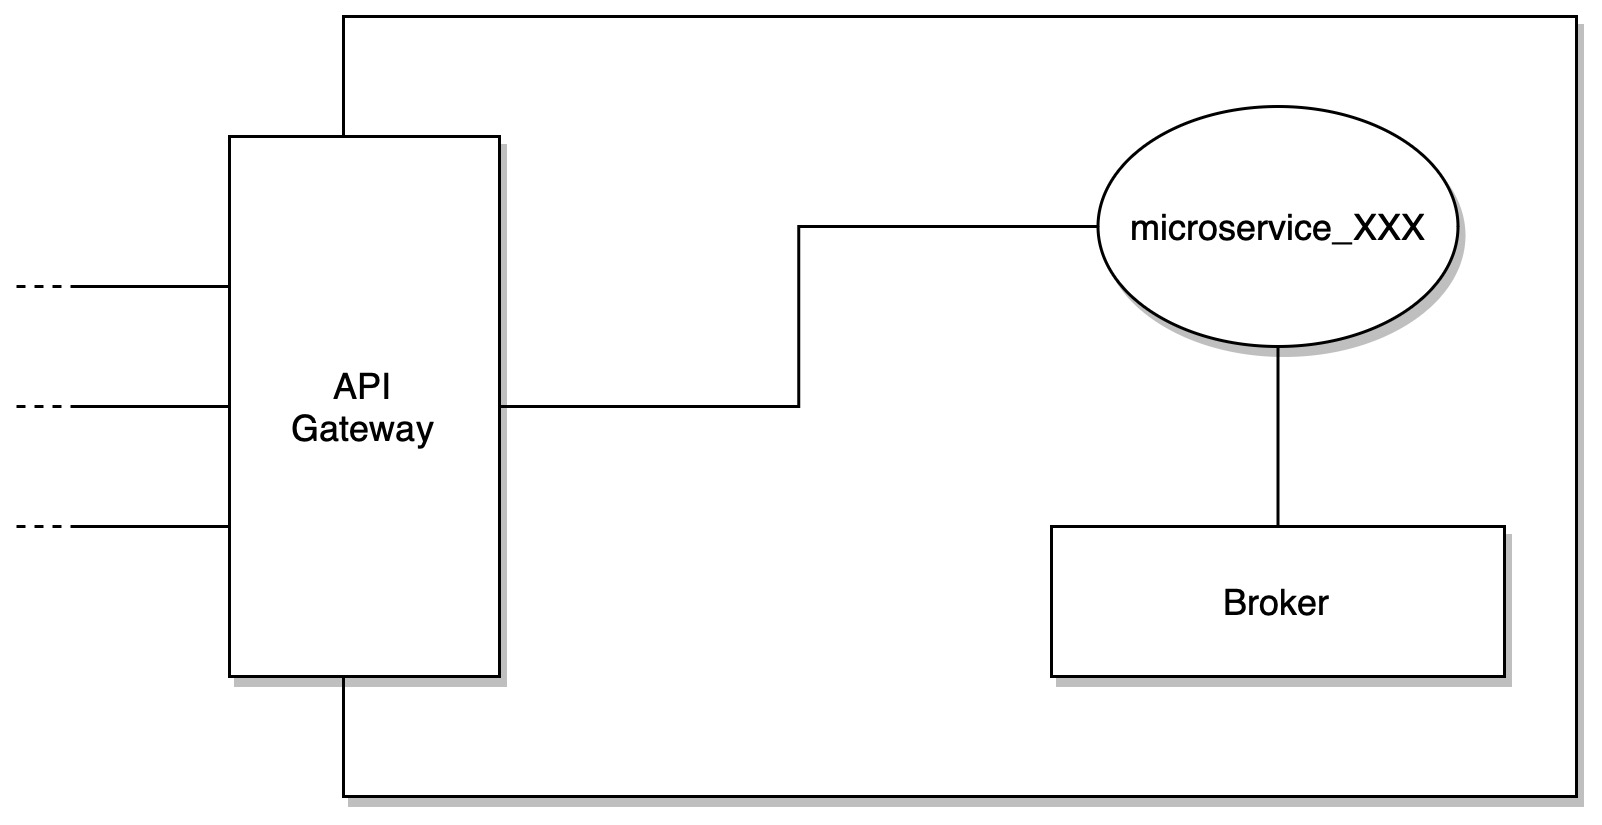
\includegraphics[width=\textwidth]{img/03-design/gateway-broker-microservice.jpg}
    \caption{Un microservizio collegato al Broker e all'API Gateway}
    \label{fig:gateway-broker-microservice}
\end{figure}

%
%
%
\subsection{L'architettura proposta}

Un utente, per accedere al servizio sfrutta l'\emph{API Gateway}.
In questo modo è possibile nascondere l'implementazione retrostante.

Di seguito è riportato lo schema architetturale del sistema.

\begin{figure}[htbp]
    \centering
    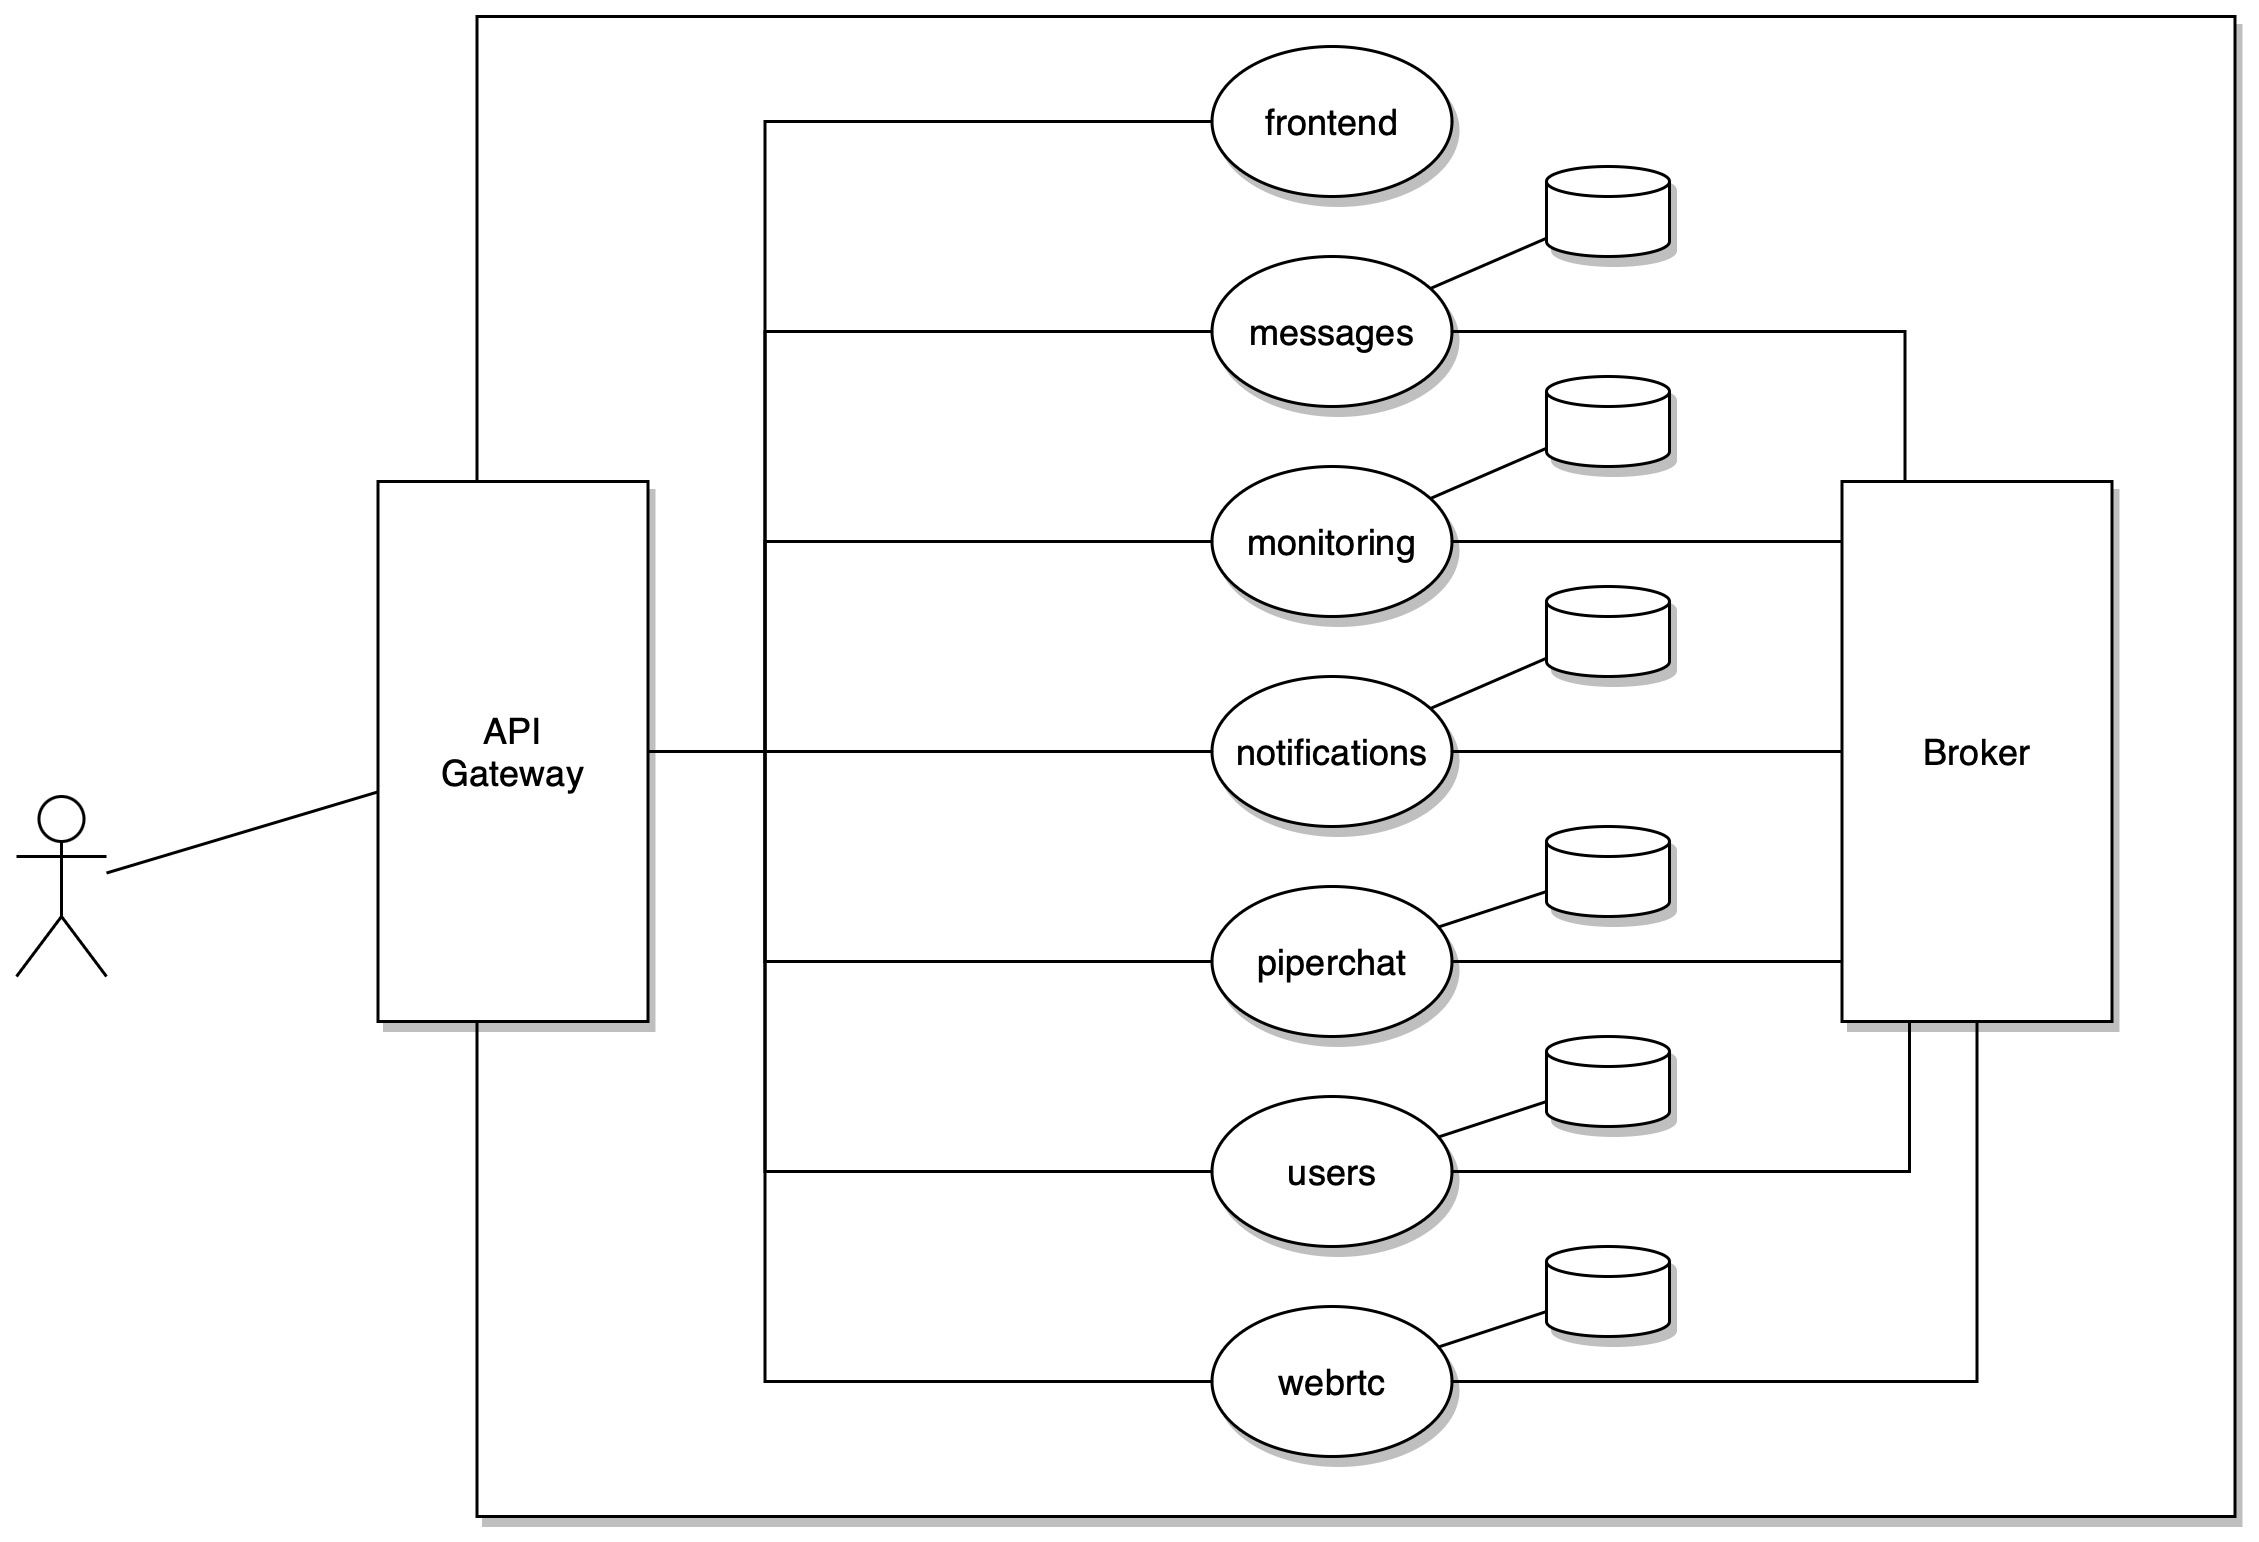
\includegraphics[angle=-90,width=0.95\textwidth]{img/03-design/architecture-schema.jpg}
    \caption{Architettura di Piperchat}
    \label{fig:piperchat-architecture}
\end{figure}

\section{Dettagli implementativi}

% Just report interesting / non-trivial / non-obvious implementation details.

% This section is expected to be short in case some documentation (e.g. Javadoc or Swagger Spec) has been produced for the software artefacts.
% %
% This this case, the produced documentation should be referenced here.

\subsection{Documentazione}

%
%
%
\subsubsection{Swagger}
Swagger è un insieme di strumenti open source per progettare, creare, documentare e consumare servizi web RESTful, attraverso la specifica \emph{Open API}.
%
L'obiettivo principale di Swagger è semplificare e standardizzare il processo di sviluppo e integrazione di API, fornendo una documentazione interattiva e uno strumento per testare direttamente le API.

Le caratteristiche chiave di Swagger includono:

\begin{itemize}
    \item Definizione della API: Swagger utilizza il formato YAML o JSON per definire la struttura e i dettagli di un'API RESTful, specificando risorse, operazioni, parametri, tipi di dati, e altro ancora.
    
    \item Interfaccia Utente Interattiva: Genera automaticamente un'interfaccia utente interattiva (Swagger UI) basata sulla definizione dell'API. Questa interfaccia consente agli sviluppatori di esplorare e testare le API direttamente dal browser.

    \item Standardizzazione e Conformità: Swagger promuove la standardizzazione nelle API RESTful, migliorando la coerenza e la comprensione tra sviluppatori e team di sviluppo
\end{itemize}

%
%
%
\paragraph{Utilizzo}

Con Swagger, è stato possibile creare documentazione dettagliata delle API, specificando dettagli come gli endpoint, i parametri, i tipi di dati, le risposte possibili e persino esempi di richieste e risposte.

Inizialmente, lo strumento è stato utilizzato per realizzare il design del sistema, permettendo di documentare ciò che si sarebbe dovuto implementare.
%
I cicli iterativi di raffinamento hanno permesso di convergere all'attuale stato dell'\emph{API}.

La documentazione delle API del progetto è consultabile sulle Github Pages:
\url{https://zucchero-sintattico.github.io/piperchat/api/rest/}

%
%
%
\subsubsection{AsyncApi}

AsyncAPI è uno standard di specifica per la progettazione di API asincrone.
%
Simile a come OpenAPI è utilizzato per definire e documentare API sincrone, AsyncAPI è progettato specificamente per gestire le comunicazioni asincrone, come quelle basate su messaggi o eventi.

Le principali caratteristiche di AsyncAPI includono:

\begin{itemize}
    \item Comunicazioni Asincrone: AsyncAPI è progettato per modellare API che coinvolgono comunicazioni asincrone, dove la richiesta e la risposta non sono sincronizzate nel tempo.

    \item Documentazione Dettagliata: Come OpenAPI per API sincrone, AsyncAPI fornisce una specifica dettagliata per documentare aspetti come endpoint, messaggi, schemi dei dati, protocolli di trasporto e altri dettagli relativi alla comunicazione asincrona.

    \item Supporto per Protocolli Comuni: AsyncAPI supporta una varietà di protocolli comuni per la comunicazione asincrona, come MQTT, AMQP e WebSocket. Ciò consente una flessibilità nella progettazione delle API a seconda delle esigenze specifiche del progetto.
\end{itemize}

%
%
%
\paragraph{Utilizzo}

AsyncAPI è stato utilizzato come strumento di supporto e di documentazione di tutte le tipologie di messaggi rappresentanti gli eventi che vengono scambiati tramite il broker all'interno dell'architettura a microservizi.

La documentazione delle API per i messaggi \textit{infra-servizi} è consultabile sulle Github Pages:
\url{https://zucchero-sintattico.github.io/piperchat/api/infra-service/}

Inoltre, la tecnologia è stata sfruttata anche per la documentazione dei messaggi \textit{inviati ai client} come notifiche di eventi.
Tale documentazione è disponibile al seguente link:
\url{https://zucchero-sintattico.github.io/piperchat/api/notification/}

%
%
%
\subsection{View}

Per la realizzazione del software in oggetto, abbiamo fatto ampio uso del framework \emph{Vue.js}\footnote{\url{https://vuejs.org}}, un potente e flessibile framework JavaScript per la costruzione di interfacce utente moderne e reattive.
%
Vue.js si è rivelato una scelta eccellente per la nostra applicazione, offrendo una struttura chiara e modulare che ha semplificato lo sviluppo e la manutenzione del codice.
%
La sua capacità di gestire in modo efficiente la visualizzazione dinamica dei dati e la reattività dell'interfaccia utente ha contribuito in modo significativo a garantire un'esperienza utente fluida e coinvolgente.

%
%
%
\subsubsection{Pinia}

\emph{Pinia JS}\footnote{\url{https://pinia.vuejs.org}} è una libreria di gestione dello stato progettata per applicazioni Vue.js.
%
Essa fornisce un'architettura di gestione dello stato centralizzata e reattiva, offrendo uno store centralizzato per memorizzare e gestire lo stato dell'applicazione.
%
Pinia si basa sui concetti principali di Vue.js, come la reattività e la gestione delle modifiche dello stato in modo efficiente.
%
Questo strumento consente agli sviluppatori di scrivere codice pulito e manutenibile, facilitando la gestione dello stato dell'applicazione Vue.js.

%
%
%
\subsubsection{Quasar}

\emph{Quasar}\footnote{\url{https://quasar.dev}} è un framework open-source basato su Vue.js, progettato per semplificare lo sviluppo di applicazioni web e mobile con un unico codice sorgente.
%
È noto per la sua flessibilità e la capacità di generare applicazioni per diverse piattaforme.
%
Le caratteristiche principali di Quasar Framework includono:

\begin{enumerate}
    \item \textbf{Componenti Vue.js predefiniti}: Quasar offre una vasta libreria di componenti Vue.js personalizzati e ricchi di funzionalità, che semplificano la creazione di interfacce utente sofisticate.

    \item \textbf{Responsive Design}: Le applicazioni Quasar possono essere facilmente rese responsive per adattarsi a diversi dispositivi e dimensioni dello schermo.

    \item \textbf{Material Design}: Quasar aderisce a Material Design di Google, offrendo un aspetto moderno e uniforme per le applicazioni.
\end{enumerate}

%
%
%
\subsection{Api Gateway}

\subsubsection{Traefik}

\emph{Traefik}\footnote{\url{https://traefik.io/traefik/}} è un moderno \emph{reverse proxy} e \emph{load balancer} progettato per gestire il traffico web in ambienti complessi e distribuiti.

%
%
%
\paragraph{Utilizzo}

Nel contesto del nostro progetto, l'utilizzo di Traefik è stato utilizzato per realizzare un \emph{API Gateway}, instradando e distribuendo il traffico tra il frontend e i diversi microservizi del backend.
%
All'interno di ciascun file \emph{Docker Compose} relativo ai singoli servizi, sono state specificate le rotte accettate dal microservizio attraverso l'aggiunta di una \emph{label}\footnote{\url{https://doc.traefik.io/traefik/providers/docker/\#routing-configuration-with-labels}}.
%
Questo approccio ci ha permesso di configurare facilmente e in modo dettagliato le direttive per il routing del traffico verso ciascun servizio, consentendo a Traefik di instradare le richieste in base alle specifiche esigenze di ciascun microservizio.

Di seguito è riportato un esempio della definizione delle rotte.

\begin{verbatim}
# Compose file

service:
  users-service:
    ...
    labels:
      - |
        traefik.http.routers.users-service.rule=
        (Method(`GET`) && Path(`/friends`)) ||
        (Method(`GET`) && Path(`/whoami`)) ||
        (Method(`GET`, `POST`) && Path(`/friends/requests`)) ||
        ...
\end{verbatim}

%
%
%
\subsection{Gestione comunicazione persistente}

Per quanto riguarda la gestione delle comunicazioni persistenti tra backend e client è stata utilizzata la libreria \emph{Socket.io}, impiegata sia nel servizio di notifiche che nel servizio multimediale per propagare i messaggi nel protocollo di join di una sessione multimediale.

%
%
%
\subsubsection{Socket.io}

Socket.IO è una libreria JavaScript che fornisce una comunicazione bidirezionale in tempo reale tra il server e il client in applicazioni web.
%
È spesso utilizzata per implementare funzionalità di chat, giochi multiplayer, aggiornamenti in tempo reale e altre applicazioni che richiedono una comunicazione immediata tra il server e il browser.
%
Le principali caratteristiche di Socket.IO per cui è stato scelto come framework sono:

\begin{itemize}
    \item \textbf{Comunicazione in tempo reale}: una comunicazione bidirezionale in tempo reale, consentendo agli utenti di ricevere aggiornamenti istantanei dal server.

    % \item \textbf{Supporto multipiattaforma}: Socket.IO è compatibile con diverse piattaforme e browser, consentendo una comunicazione uniforme su molteplici dispositivi.

    % \item \textbf{Messaggi personalizzati}: Gli sviluppatori possono definire messaggi personalizzati per gestire eventi specifici nell'applicazione, come messaggi di chat o aggiornamenti di gioco.

    \item \textbf{Riconnessione automatica}: è supportata la riconnessione automatica in caso di perdita di connessione, garantendo che gli utenti rimangano connessi.

    % \item \textbf{Ampia adozione}: Socket.IO è ampiamente utilizzato nella comunità di sviluppatori ed è supportato da molte piattaforme e framework.

\end{itemize}

%
%
%
\subsubsection{Notifications Service: notifiche e gestione status}

Un utente, quando si connette al sistema, deve essere considerato online e deve essere abilitato alla ricezione delle notifiche.

Date queste premesse, viene instaurata, tra il server e il client autenticato, una connessione tramite Socket.IO.
%
Si è deciso di collassare, all'interno di questa socket, le due responsabilità:

\begin{enumerate}
    \item Permettere al server di inviare notifiche ai client.

    \item Finché la socket è aperta, il client viene considerato online.
\end{enumerate}

%
%
%
\paragraph{Considerazioni su scalabilità e stato persistente}

Dal momento che il microservizio mantiene uno stato, la scalabilità orizzontale potrebbe non essere ovvia.
%
Di seguito vengono analizzate le considerazioni effettuate al fine di permettere la scalabilità orizzontale, senza incorrere in inconsistenze.

%
%
%
\subparagraph{Utente stabilisce la connessione} 

Quando un utente fa richiesta verso il servizio di notifica, instaura una socket verso una specifica replica.
%
Questa replica sarà colei che manterrà la connessione persistente verso l'utente.
%
Inoltre, essa si occupa di aggiornare lo status (online/offline) nel database condiviso con le altre repliche.

%
%
%
\subparagraph{Nuovo evento per un utente}

Quando un nuovo evento viene generato nel sistema ed un utente, deve essere notificato.
%
Il broker invierà in broadcast l'evento a tutte le copie del servizio, ma sarà solo la replica che mantiene la connessione persistente ad inviare al client l'opportuna notifica.

%
%
%
\subparagraph{Richiesta dello status di un utente}

Quando un utente qualsiasi richieste lo stato di un altro utente, qualsiasi replica può assolvere a questa richiesta dal momento che lo status è salvato nel database condiviso.

\begin{figure}[H]
    \centering
    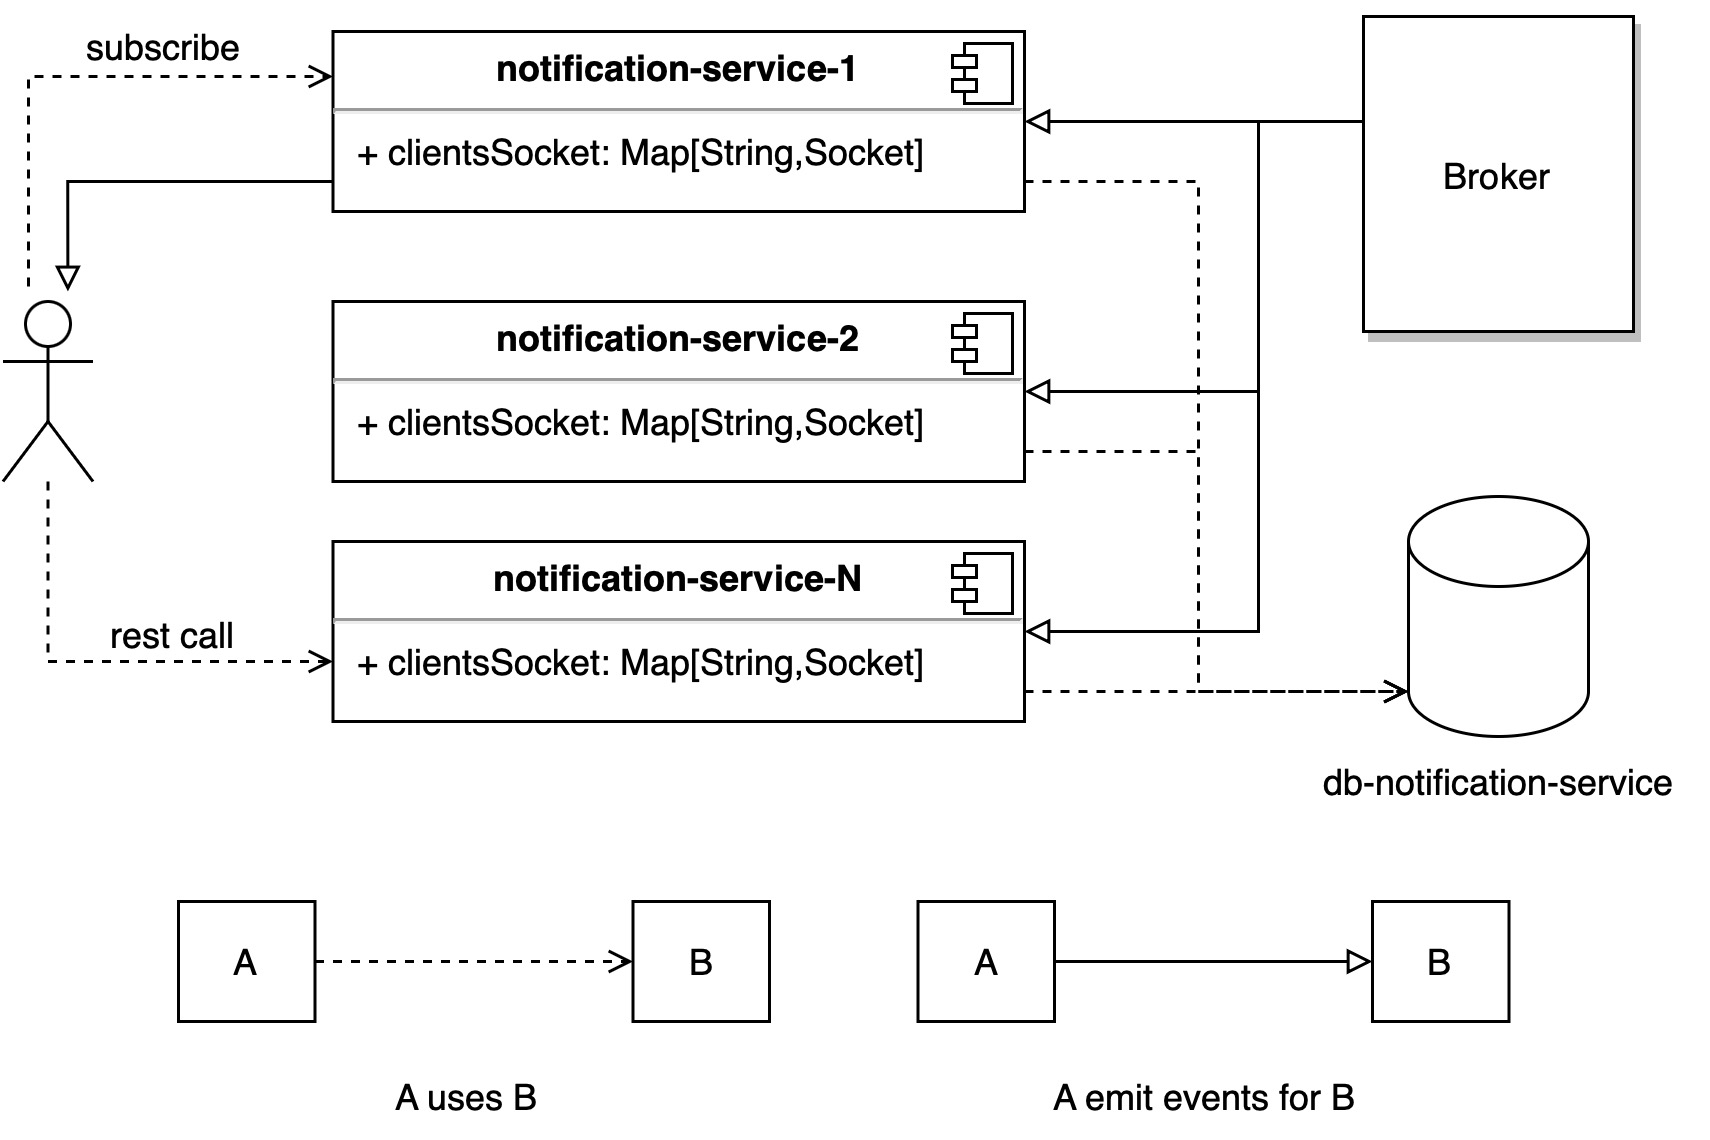
\includegraphics[width=\textwidth]{sections/04-implementation/img/notification-replication.jpg}
    \caption{Un utente crea una connessione persistente}
\end{figure}

%
%
%
\subsubsection{Socket.IO vs Server Sent Event}

Durante le fasi iniziali del progetto, al fine di inviare le notifiche dal microservizio verso il client, era stata adottato \emph{Server-Sent Events}\footnote{\url{https://developer.mozilla.org/en-US/docs/Web/API/Server-sent_events}}, una tecnologia di comunicazione monodirezionale, che permette di ricevere dati da un server che li invia.

Questo approccio è stato successivamente sostituito da Socket.IO perché il server non può gestire in modo responsivo la chiusura di una connessione da parte del client.

%
%
%
\subsection{WebRTC}

\emph{WebRTC}\footnote{\url{https://developer.mozilla.org/en-US/docs/Web/API/WebRTC_API}}, acronimo di “Web Real-Time Communication", è una tecnologia open-source che consente la comunicazione audio e video in tempo reale direttamente tra browser web senza richiedere plugin o software aggiuntivi.
%
È utilizzato per creare applicazioni di videoconferenza, chat video, streaming multimediale e altro.

Le principali caratteristiche di WebRTC includono:

\begin{enumerate}
    \item \textbf{Comunicazione peer-to-peer}: WebRTC consente ai browser di comunicare direttamente tra loro, evitando la necessità di server intermediari per la trasmissione di dati in tempo reale.

    \item \textbf{Supporto per audio e video}: WebRTC supporta la comunicazione audio e video in tempo reale, consentendo agli utenti di interagire tramite chat video o conferenze online.

    \item \textbf{Accesso ai dispositivi}: WebRTC consente l'accesso ai dispositivi hardware come telecamere e microfoni per abilitare la cattura audio e video.
\end{enumerate}

%
%
%
\subsubsection{Funzionamento}
Nel contesto di WebRTC, ci sono tre concetti chiave: \textbf{offer}, \textbf{answer}, e \textbf{ICE candidates}.

\begin{itemize}
    \item \textbf{Offer}:
    L'offerta è il punto di partenza per l'inizializzazione di una connessione WebRTC.

    Un peer (la parte che inizia la connessione) crea un'offerta che specifica le sue preferenze per la sessione di comunicazione, inclusi i codec supportati, i parametri di sicurezza, etc.
    L'offerta è creata utilizzando l'API \textit{createOffer().}

    \item \textbf{Answer}:
    L'answer è generata dal peer destinatario in risposta all'offerta ricevuta.
    %
    Il peer destinatario, dopo aver ricevuto l'offerta, crea una risposta che riflette le sue preferenze per la comunicazione.
    L'answer è creata utilizzando l'API \textit{createAnswer().}

    \item \textbf{ICE Candidates}:
    ICE (Interactive Connectivity Establishment) è un protocollo utilizzato per stabilire una connessione in presenza di reti complesse, come dietro firewall o NAT.
    I candidati ICE sono gli indirizzi IP e le porte su cui un peer può essere contattato.
    Durante il processo di offerta e risposta, i peer scambiano i loro candidati ICE utilizzando l'API \textit{onIceCandidate()}.
    Il processo di raccolta dei candidati ICE è noto come “ICE gathering".
\end{itemize}

In sintesi, il flusso tipico di inizializzazione di una connessione WebRTC coinvolge la creazione di un'offerta da parte del peer iniziatore, la trasmissione di questa offerta al peer destinatario, la creazione di una risposta da parte del peer destinatario e, infine, lo scambio di candidati ICE per stabilire una connessione diretta tra i due peer.
%
Questo processo è fondamentale per consentire la comunicazione bidirezionale in tempo reale tra browser senza passare attraverso un server intermedio.

%
%
%
\subsubsection{Sessione multimediale}
La gestione delle sessioni per le videochiamate WebRTC si basa su un modello che prevede l'utilizzo di sessioni individuali, ciascuna identificata da un unico ID e caratterizzata da un insieme di utenti consentiti (“allowed users") e dagli attuali partecipanti durante la chiamata in corso.
%
Ogni amicizia tra utenti è associata a una propria sessione, e lo stesso vale per i canali multimediali, i quali fanno riferimento a una sessione per agevolare le chiamate multimediali.

Le sessioni vengono distintamente gestite in base al contesto.
%
Nel caso delle amicizie, l'insieme di utenti consentiti è limitato esclusivamente ai due partecipanti dell'amicizia, garantendo una comunicazione privata tra i diretti interessati.
%
Invece, nei canali multimediali, l'insieme di utenti consentiti comprende tutti i partecipanti del server, consentendo così chiamate multimediali che coinvolgono più membri contemporaneamente.

Questo approccio alla gestione delle sessioni offre un controllo granulare sull'accesso alle videochiamate, garantendo che la comunicazione sia personalizzata in base al contesto delle relazioni tra gli utenti.
%
Inoltre, consente una scalabilità efficiente per le chiamate multimediali su larga scala, consentendo a tutti i partecipanti del server di partecipare alle conversazioni senza compromettere la sicurezza o la privacy delle comunicazioni one-to-one.

%
%
%
\subsubsection{Protocollo Signaling}

Di seguito il protocollo utilizzato per la procedura di signaling webrtc che permette lo scambio delle informazioni necessarie all instauramento delle connessioni p2p. 

\begin{figure}[H]
    \centering
    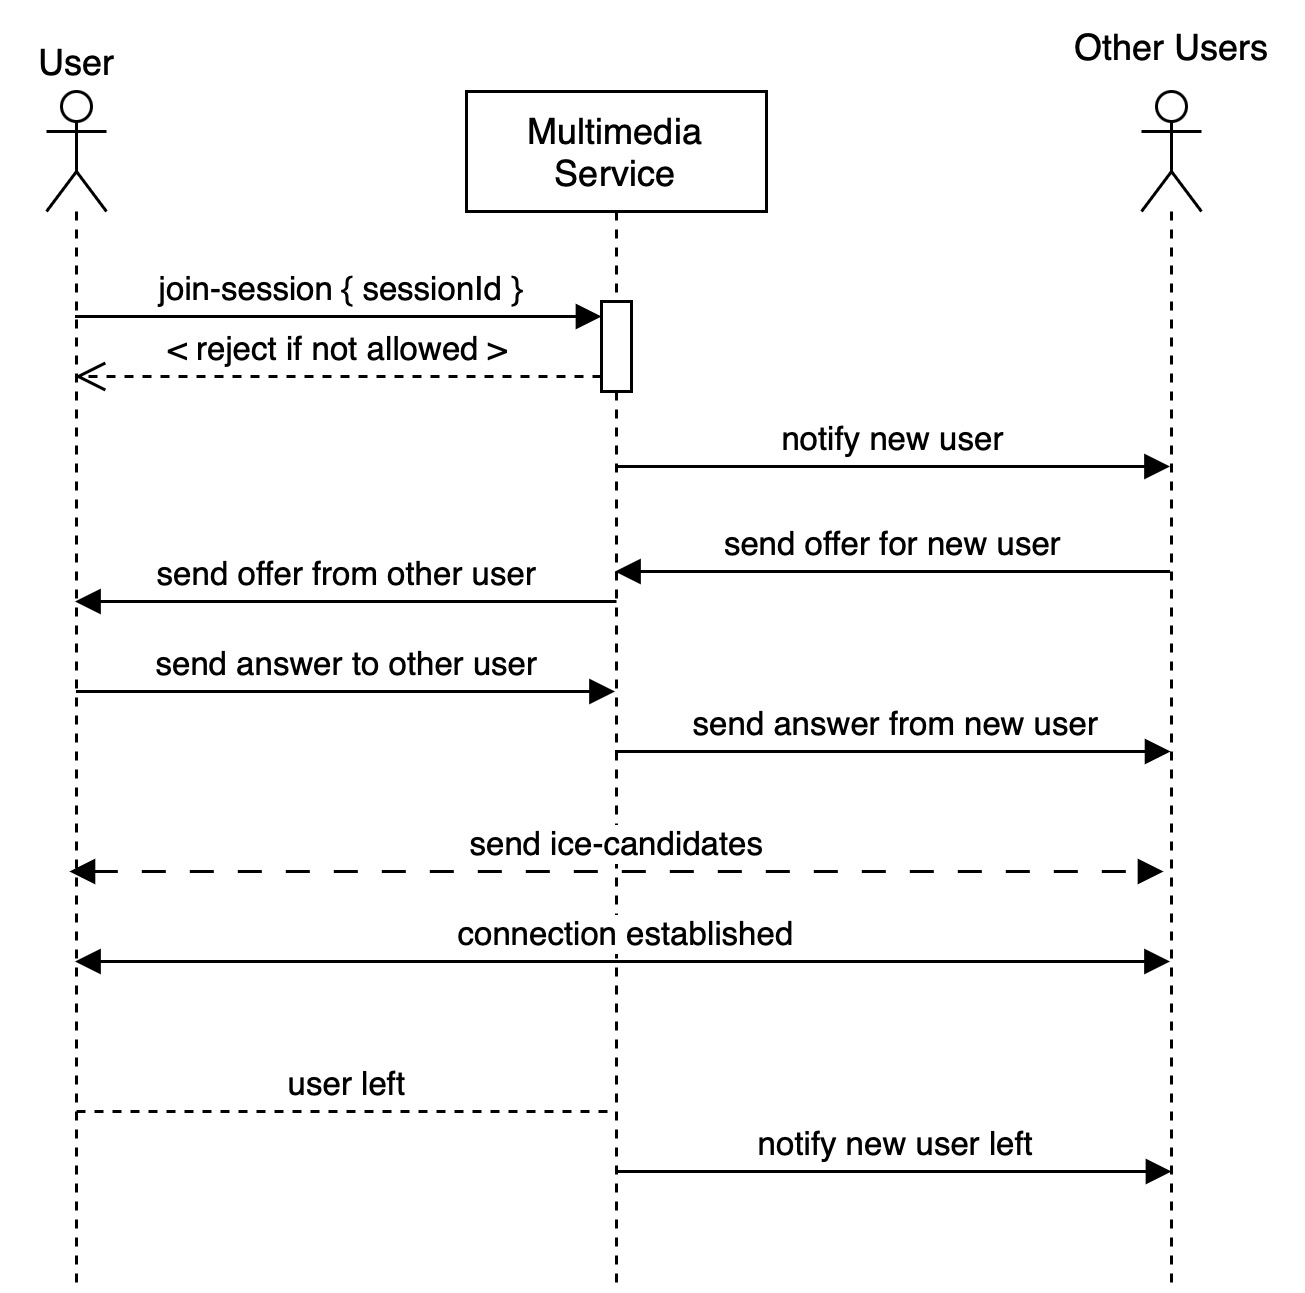
\includegraphics[width=0.9\textwidth]{sections/04-implementation/img/piperchat-Multimedia.jpg}
    % \caption{Protocollo signaling sessioni multimediali}
    \label{fig:piperchat-signaling}
\end{figure}

%
%
%
\subsubsection{Problema P2P e TURN}

Uno dei problemi principali che WebRTC deve affrontare è la presenza di dispositivi di rete con NAT (Network Address Translation) non compatibili, che possono complicare la creazione di connessioni dirette tra i partecipanti.

Il NAT consente a più dispositivi di condividere un singolo indirizzo IP pubblico, fornendo una forma di sicurezza e limitando la quantità di traffico Internet diretto verso dispositivi locali. Tuttavia, questo può creare problemi quando si tenta di stabilire connessioni dirette tramite WebRTC, in quanto alcuni NAT possono impedire il passaggio dei pacchetti dati necessari.

Per superare questo problema, WebRTC utilizza un concetto chiamato \textit{Traversal Using Relays around NAT (TURN)}. Un server TURN agisce come intermediario tra i partecipanti, aiutando a instradare i dati quando le connessioni dirette non sono possibili. Quando due peer non possono stabilire una connessione diretta a causa di NAT non compatibili, i dati vengono instradati attraverso il server TURN, consentendo comunque la comunicazione in tempo reale.

Per ovviare a questa problematica è stato quindi aggiunto al deploy anche un servizio adibito a funzionare da TURN in caso non sia possibile la connessione p2p.

%
%
%
\subsection{Autenticazione degli utenti}

Per gestire l'autenticazione degli utenti all'interno del nostro sistema, è stata adottata la tecnologia \textit{JSON Web Token (JWT)}.

%
%
%
\subsubsection{JWT}

JSON Web Token (JWT) è uno standard aperto (RFC 7519) che definisce un modo compatto per rappresentare informazioni tra due parti.
%
Queste informazioni possono essere verificate e fidate, poiché sono firmate digitalmente.

%
%
%
\paragraph{Struttura dei JWT}

Un JWT è costituito da tre parti separate da punti (.), che sono:

\begin{itemize}
    \item \textbf{Header:} Contiene il tipo di token (che è JWT) e l'algoritmo di firma utilizzato, ad esempio, HMAC SHA256 o RSA.
    
    \item \textbf{Payload:} Contiene le dichiarazioni, chiamate anche \textit{claim}, che rappresentano l'entità (solitamente l'utente) e le informazioni aggiuntive. %Esistono tre tipi di claim: registrati, pubblici e privati.
    
    \item \textbf{Signature:} Per ottenere la firma, si prende l'header codificato, il payload codificato, una chiave segreta, e si applica un algoritmo specifico. Questa firma viene aggiunta al token.
\end{itemize}

%
%
%
\paragraph{Funzionamento}

Quando un utente si autentica, riceve un JWT che può includere informazioni come l'identità e i diritti di accesso. Da quel momento in poi, il client invia il JWT con ogni richiesta successiva al server, che può verificare la firma del token per assicurarsi che sia valido. In questo modo, il server può fidarsi delle informazioni contenute nel JWT senza doverle verificare ad ogni richiesta.

%
%
%
\paragraph{Utilizzo}

Nel contesto di Piperchat, quando un utente si autentica con successo, il microservizio \texttt{Users} genera un JWT contenente nel payload le informazioni relative all'identità dell'utente. Questo JWT viene restituito al client, che lo utilizzerà nelle successive richieste per dimostrare la propria autenticità.

Inoltre, viene memorizzato nel database un token di refresh, che consente di ottenere nuovi token di accesso senza dover effettuare nuovamente l'accesso.

Quando il token di accesso scade, il client può richiedere un nuovo token di accesso al server utilizzando il token di refresh. Questo processo aiuta a mantenere un'esperienza utente fluida, riducendo al contempo il rischio di accessi non autorizzati.

%In sintesi, l'utilizzo di JSON Web Token all'interno di PiperChat offre un meccanismo robusto per l'autenticazione degli utenti, facilitando al contempo la gestione dei token sia lato client che lato server.

%
%
%
\subsection{Definizione delle API}

Per quanto riguarda la gestione delle api dei vari microservizi si è optato per avere una struttura che rappresentasse ogni endpoint, incapsulando sia i dati richiesti sia le possibili risposte.

A supporto di ciò è stato creato un modulo \textbf{api} che incapsula tutti gli endpoint del backend con le relativi informazioni.

Tale modulo viene sfruttato sia dal backend, per avere un typing migliore e un controllo di validazione dei parametri richiesti, che dal frontend per sapere già quali sono codice di risposta e tipologie di risposta per un determinato endpoint.

\begin{lstlisting}[style=typescript, caption={Definizione API}, label=lst:login:api]
export module LoginApi {

  export module Request {
    export type Body = {
      username: string
      password: string
    }
    export const Schema: RequestSchema = {
      Body: {
        username: 'string',
        password: 'string',
      },
    }
  }

  export module Responses {
    export class Success extends Response {
      statusCode = 200
      message = 'Logged in' as const
      jwt: string
    }
  }

  export module Errors {
    export class UsernameOrPasswordIncorrect extends ErrorResponse {
      statusCode = 401
      error = 'Username or password incorrect' as const
    }
  }
}
\end{lstlisting}

%
%
%
\subsection{Definizione degli Endpoint}

Una volta costruita la struttura rappresentante le singole API è stata creata l'utility \textbf{Route}, che a partire da un api permette di implementare l'endpoint aggiungendo il supporto automatico alla validazione dei dati in modo che se i dati in ingresso non dovessero essere corretti,  l'handler non venga notificato e venga restituito un messaggio di errore \textit{Bad Request}.
%
Inoltre permette e di dichiarare come reagire per ogni tipo di errore senza doverli controllare all'interno dell'handler.

Altra utilità offerta dalla classe è il typing dei parametri della richiesta basati sulle api specificate.

\begin{lstlisting}[style=typescript, caption={Definizione API}, label=lst:login:route]
export const LoginApiRoute = new Route<
  ...
>({
  method: 'post',
  path: '/login',
  schema: LoginApi.Request.Schema,
  handler: async (req, res) => {
    const token = await authController.login(req.body.username, req.body.password)
    res.sendResponse(new LoginApi.Responses.Success(token))
  },
  exceptions: [
    {
      exception: InvalidUsernameOrPassword,
      onException: (e, req, res) => {
        res.sendResponse(new UsernameOrPasswordIncorrect())
      },
    },
  ],
})
\end{lstlisting}

%
%
%
\subsection{Definizione dei Controller}

Per interfacciarsi con gli endpoint del backend sono quindi stati realizzati i \textbf{Controller} lato frontend, che incapsulano la gestione delle API fruttando il modulo opportuno per ottenere un typing delle richieste e delle risposte.

\begin{lstlisting}[style=typescript, caption={Definizione Controller}, label=lst:controller]
export class AuthControllerImpl extends AxiosController implements AuthController {
  async register(request: RegisterApi.Request.Type): Promise<RegisterApi.Response> {
    const body = request as RegisterApi.Request.Body
    return await this.post<RegisterApi.Response>('/auth/register', body)
  }

  async login(request: LoginApi.Request.Type): Promise<LoginApi.Response> {
    const body = request as LoginApi.Request.Body
    return await this.post<LoginApi.Response>('/auth/login', body)
  }

  async logout(): Promise<LogoutApi.Response> {
    return await this.post<LogoutApi.Response>('/auth/logout', {})
  }

  async refreshToken(): Promise<RefreshTokenApi.Response> {
    return await this.post<RefreshTokenApi.Response>(
        '/auth/refresh-token', {})
  }
}
\end{lstlisting}

%
%
%
\subsection{Monitoring}

Per monitorare lo stato dei servizi, è stato esposto un endpoint che restituisce un oggetto JSON contenente lo stato corrente e l'orario dell'ultimo aggiornamento.
%
Per garantire l'aggiornamento continuo del client rispetto a queste informazioni, si è optato per l'implementazione di un meccanismo di polling dal client al server.
%
Questa scelta consente al client di mantenere costantemente aggiornato lo stato dei servizi, anche nel caso in cui il server o i singoli microservizi diventino temporaneamente indisponibili.
%
In questo modo, il comportamento del client rimarrà invariato, assicurando una sincronizzazione continua con lo stato più recente dei servizi monitorati.
%
Inoltre, il microservizio di monitoraggio effettua anch'esso polling nei confronti degli altri microservizi per verificare se riceve risposta o meno.

\begin{lstlisting}[style=typescript, caption={Monitoring Polling - Client}, label=lst:ClientMonitoringPolling]
onMounted(async () => {
  await monitoringStore.refreshServicesStatus()
  setInterval(monitoringStore.refreshServicesStatus, 2000)
})
\end{lstlisting}

\subsection{Recap tecnologie utilizzate}

Di seguito un elenco di tutte le tecnologie utilizzate all'interno del progetto:

\subsubsection{Infrastruttura}
\begin{itemize}
    \item \textit{Docker} per il deploy dei container.
    \item \textit{Traefik} come Api-Gateway.
    \item \textit{RabbitMQ} come Broker.
\end{itemize}

\subsubsection{Microservizio}
\begin{itemize}
    \item \textit{NodeJS} come runtime environment.
    \item \textit{Typescript} come linguaggio di sviluppo.
    \item \textit{Express} per lo sviluppo dei Webserver.
    \item \textit{MongoDB} come database.
    \item \textit{Mongoose} come libreria per l'utilizzo di database Mongo.
    \item \textit{JWT} per la gestione dell'autenticazione.
    \item \textit{Jest} come framework di Unit testing.
\end{itemize}

\subsubsection{Frontend}
\begin{itemize}
    \item \textit{Vue.js} per lo sviluppo della Single Page Application.
    \item \textit{Pinia} per la gestione degli store.
    \item \textit{Quasar} per la realizzazione dei componenti grafici.
\end{itemize}

\subsubsection{Comunicazione}
\begin{itemize}
    \item \textit{Axios} per la gestione di richieste HTTP.
    \item \textit{Socket.io} per le comunicazioni real-time.
    \item \textit{WebRTC} per le videochiamate.
\end{itemize}

\subsubsection{Documentazione}
\begin{itemize}
    \item \textit{Swagger} per la documentazione delle API.
    \item \textit{AsyncAPI} per la documentazione dei messaggi infra-servizio.
\end{itemize}
\section{Autovalutazione / Validazione}

% Choose a criterion for the evaluation of the produced software and \textbf{its compliance to the requirements above}.

% Pseudo-formal or formal criteria are preferred.

% In case of a test-driven development, describe tests here and possibly report the amount of passing tests, the total amount of tests and, possibly, the test coverage.

%
%
%
\subsection{Struttura del repository e analisi statica}

Il progetto è stato sviluppato adottando una struttura \texttt{mono repository - multi project}.
%
Per garantire la coerenza, la qualità e la manutenibilità del codice sorgente, durante lo sviluppo abbiamo seguito \textbf{GitFlow} e adottato fin da subito diversi strumenti per l'analisi statica. 
%
Inoltre, al fine rendere estendibile e meno prolissa la manutenibilità di ogni progetto, sono stati adottati meccanismi di estensione nei file di configurazione.

%
%
%
\subsubsection{Lint}

Come strumento di Linting abbiamo adottato \emph{ESLint}\footnote{\url{https://eslint.org}}, grazie al quale, il nostro team ha potuto identificare e correggere errori, migliorare la coerenza del codice e rispettare le best practices di programmazione durante il processo di sviluppo.

%
%
%
\subsubsection{Prettier}

\emph{Prettier}\footnote{\url{https://prettier.io}} è uno strumento per la formattazione del codice, integrato nel nostro flusso di lavoro per garantire uno stile uniforme in tutto il progetto.
%
Le principali considerazioni includono:

\begin{itemize}
  \item \textbf{Configurazione condivisa:} lo strumento è configurato per seguire uno stile condiviso in tutto il progetto, garantendo coerenza nella formattazione del codice.

  \item \textbf{Integrazione con ESLint:} la configurazione di Prettier è allineata con quella di ESLint, evitando conflitti e assicurando una formattazione coerente durante l'analisi statica.
\end{itemize}

L'utilizzo di Prettier ha migliorato la leggibilità del codice e semplificato notevolmente la gestione dello stile del codice degli artefatti.

%
%
%
\subsubsection{Pre-commit Hook (Git)}

Gli \emph{hooks} di Git\footnote{\url{https://git-scm.com/book/it/v2/Customizing-Git-Git-Hooks}} sono strumenti che permettono di eseguire automaticamente azioni specifiche al verificarsi di eventi.

È stato utilizzato l'hook di \emph{pre-commit}, al fine di eseguire controlli di formattazione prima di eseguire un commit.
%
Questo ha permesso di migliorare la qualità del codice, evitando commit con formattazione non conforme.
%
% Nel nostro progetto, li utilizziamo per eseguire alcuni controlli preventivi prima di immagazzinare le modifiche nel repository. Le considerazioni principali includono:

% \begin{itemize}
%   \item \textbf{Configurazione Customizzata:} Abbiamo configurato hook pre-commit per eseguire linting e formattazione automatica del codice prima di ogni commit.
%   \item \textbf{Integrazione con ESLint e Prettier:} I hook pre-commit sono integrati con ESLint e Prettier, assicurando che il codice sorgente rispetti le regole di linting e formattazione prima di essere immagazzinato.
% \end{itemize}

%
%
%
\subsection{Testing}

La fase di testing è strutturata per verificare l'integrazione tra l'intero microservizio e le sue dipendenze, tra cui il Database e il Broker.

% \begin{itemize}
%     \item Il Database
%     \item Il Broker
% \end{itemize}

%
%
%
\subsubsection{Jest}

Ogni microservizio definisce degli \emph{Unit Testing} mediante \emph{Jest} in modo da verificare la correttezza delle richieste e delle relative risposte, dei singoli microservizi.

In questo modo, siamo stati in grado di concentrarci sui seguenti aspetti durante i test:

\begin{itemize}
    \item Verifica della correttezza delle richieste fornite.

    \item Verifica della correttezza delle risposte fornite da diverse richieste.

    \item Verifica della correttezza che gli endpoint si comportino come atteso, controllando i \emph{side effect} di una richiesta, eseguendo richieste successive.
\end{itemize}

Questo approccio ci ha permesso di sviluppare test solidi e garantire che i microservizi rispettassero gli standard richiesti.

%
%
%
\subsubsection{Test sui Microservizi}

Tutti i microservizi posseggono una suite di test.
%
Di seguito un esempio con il core del testing del servizio degli utenti:

\begin{lstlisting}[style=typescript, caption={microservice Test}, label=lst:login:route:test]
const userMicroservice: Microservice = new Microservice(UserServiceConfiguration)
let request: supertest.SuperTest<supertest.Test>

beforeAll(async () => {
  await userMicroservice.start()
  request = supertest(userMicroservice.getServer())
})

afterAll(async () => {
  await userMicroservice.stop()
})

afterEach(async () => {
  await userMicroservice.clearDatabase()
})

describe('Register', () => {
  it('A user must provide username, password and email', async () => {
    let response = await request
      .post('/auth/register')
      .send({ username: 'test', password: 'test' })
    expect(response.status).toBe(400)
    // other test stuff
    response = await request
      .post('/auth/register')
      .send({ username: 'test', password: 'test', email: 'test' })
    expect(response.status).toBe(200)
  })
    // other test stuff
})
\end{lstlisting}

% describe('Login', () => {
%     it('A user should provide username and password to login', async () => {
%         let response = await register('test', 'test', 'test')
%         response = await request.post('/auth/login').send({ username: 'test' })
%         expect(response.status).toBe(400)
%         response = await request.post('/auth/login').send({ password: 'test' })
%         expect(response.status).toBe(400)
%         response = await request
%           .post('/auth/login')
%           .send({ username: 'test', password: 'test' })
%         expect(response.status).toBe(200)
%     })
%     // other test stuff
% })

% describe('Logout', () => {
%   it('A user should be able to logout', async () => {
%     let response = await createUserAndLogin('test', 'test', 'test')
%     const cookie = response.header['set-cookie']
%     response = await request.post('/auth/logout').set('Cookie', cookie)
%     expect(response.status).toBe(200)
%   })
%     // other test stuff
% })

% describe('Refresh token', () => {
%   it('A user should be able to refresh token', async () => {
%     let response = await createUserAndLogin('test', 'test', 'test')
%     const cookie = response.header['set-cookie']
%     response = await request.post('/auth/refresh-token').set('Cookie', cookie)
%     expect(response.status).toBe(200)
%     expect(response.header['set-cookie']).toHaveLength(1)
%   })
%     // other test stuff
% })

%
%
%
\subsubsection{Esecuzione dei test}

Al fine di eseguire le suite di test è necessario rendere disponibili le dipendenze dei microservizi.
%
Procedere come segue:

\begin{verbatim}
# Un terminale (directory = projectRoot)
npm i
cd dev
./runDev.sh

# Altro terminale (e.g. test su microservizio users)
npm run --workspace services/users test
# oppure (per eseguire tutti i test)
npm run test
\end{verbatim}

%
%
%
\subsection{Continuous Integration}

Il progetto è ospitato in due servizi di hosting: GitHub e GitLab.
%
Il primo servizio è stato utilizzato per l'intera fase di sviluppo, mentre il secondo meramente per eseguire una copia all'interno del repository fornito per il progetto.

%
%
%
\subsubsection{Github Action}

Le \emph{GitHub Actions} sono un sistema di automazione integrato direttamente nella piattaforma \emph{GitHub}, il servizio di hosting scelto per ospitare la fase di sviluppo del progetto.

Sono stati realizzati i seguenti workflow:

\begin{itemize}
    \item \textbf{\href{https://github.com/zucchero-sintattico/piperchat/blob/develop/.github/workflows/check-style.yaml}{Check code style and lint}:} il workflow esegue i controlli di analisi statica sul codice per ogni push nel repository.

    \item \textbf{\href{https://github.com/zucchero-sintattico/piperchat/blob/develop/.github/workflows/pages.yml}{Deploy pages}:} il workflow esegue il deploy del sito statico mediante \emph{GitHub Pages}.
    All'interno del sito è possibile trovare le varie api, relazione, etc.

    \item \textbf{\href{https://github.com/zucchero-sintattico/piperchat/blob/develop/.github/workflows/dispatch-services-test.yaml}{Dispatch tests}:} il workflow esegue i test di tutti i microservizi.

    \item \textbf{\href{https://github.com/zucchero-sintattico/piperchat/actions/workflows/service-unit-testing.yaml}{Testing services}:} il workflow esegue i test dei microservizi che sono stati modificati nel push che lo ha innescato.
\end{itemize}

I test automatici eseguiti all'interno dei workflows necessitano delle dipendenze sopra citate, tra cui Database e Broker.
%
Al fine di risolverle, vengono utilizzati i \texttt{services} delle GitHub Action, che permettono di istanziare gli opportuni servizi.

%
%
%
\subsubsection{Dispatch tests e Testing services}

Nell'ottica di uno sviluppo coadiuvato da un elevato numero di commit, l'idea iniziale per cui è stato realizzato il workflow \emph{Testing services} era per evitare di eseguire l'intera suite di test ad ogni push.
%
Infatti, il workflow esegue i test del microservizio modificato.
%
Il supporto fornito dalle API delle GitHub Action è limitato, infatti si è dovuto scrivere un complesso script bash.

A seguito dello sviluppo è stato constatato che ciò non era necessario questo workflow aggiuntivo, infatti, l'intera suite di test non richiede eccessivo tempo per essere eseguita.

\chapter{Deployment}

L'applicazione è strutturata mediante i seguenti container:

\begin{itemize}
    \item Frontend Service: container che serve il Frontend sotto forma di Single Page Application.

    \item Messages Service e relativo Db: servizio responsabile della gestione dei messaggi testuali dell'applicazione (invio, ricezione, ecc...).

    \item Monitoring Service e relativo Db: servizio responsabile del monitoraggio dello stato di tutti i microservizi.

    \item Notifications Service e relativo Db: servizio responsabile delle notifiche degli utenti. Inoltre, detiene l'online status degli utenti del sistema.

    \item Piperchat Service e relativo Db: servizio responsabile della gestione dei Server e dei Canali dell'applicazione (creazione, modifica, partecipanti, ecc...).

    \item Users Service e relativo Db: servizio responsabile della gestione degli utenti dell'applicazione (login, registrazione, amicizie, ecc...).

    \item WebRTC Service e relativo Db: servizio responsabile della gestione delle chiamate infra-utenti e dei canali multimediali.

    \item Broker: container che ospita un server di \emph{RabbitMQ} per permettere lo scambio di messaggi all'interno del sistema

    \item Coturn: container che ospita il server \emph{TURN} (\url{https://github.com/coturn/coturn})

    \item Gateway: container che ospita l'\emph{API Gateway} realizzato con \emph{Traefik}. 

    \item Inspector: container di \emph{utility} per debuggare e/o ispezionare i servizi dall'interno della rete.
\end{itemize}

Per ogni microservizio quindi, viene effettuato il deploy di due diversi container, uno per il Webserver, mentre l'altro per il relativo database non relazionale.

Ogni microservizio possiede le seguenti reti docker:

\begin{itemize}
    \item Frontend: Per ricevere le richieste dal frontend tramite il Gateway.

    \item Backend: Per comunicare con gli altri microservizi (nel nostro caso tramite message broker).

    \item Microservicename-network: Rete interna del microservizio, utile alla comunicazione con il proprio database.
\end{itemize}

%
%
%
\section{Microservice deploy}

Per ogni microservizio è stato scritto un file \texttt{Docker Compose}.

Esempio di Docker compose relativo al singolo microservizio:

\begin{verbatim}
services:
  piperchat-service:
    image: piperchat
    command: [
        'npm', 
        'run', 
        '--workspace', 
        './services/piperchat', 
        'start'
    ]
    expose:
      - '${PIPERCHAT_SERVICE_PORT}'
    depends_on:
      db-piperchat-service:
        condition: service_healthy
      broker:
        condition: service_healthy
    networks:
      piperchat-network:
      backend:
        aliases:
          - ${PIPERCHAT_SERVICE_NAME}
      frontend:
    environment:
      - 'PORT=${PIPERCHAT_SERVICE_PORT}'
      - 'AMQP_URI=${BROKER_URI}'
      - 'MONGO_URI=
      mongodb://db-piperchat-service:27017/piperchat'
    labels:
      - |
        traefik.http.routers.piperchat-service.rule=
        (Method(`GET`, `POST`) 
            && Path(`/servers`)) ||
        (Method(`GET`, `PUT`, `DELETE`) 
            && Path(`/servers/{serverId:[^/]+}`)) ||
        (Method(`GET`, `POST`, `DELETE`) 
            && Path(`/servers/{serverId:[^/]+}/participants`)) ||
        (Method(`DELETE`) 
            && Path(`/servers/{serverId:[^/]+}/participants/{userId:[^/]+}`)) ||
        (Method(`GET`, `POST`) 
            && Path(`/servers/{serverId:[^/]+}/channels`)) ||
        (Method(`GET`, `PUT`, `DELETE`) 
            && Path(`/servers/{serverId:[^/]+}/channels/{channelId:[^/]+}`))

  db-piperchat-service:
    image: mongo
    expose:
      - '27017'
    volumes:
      - './.docker/db-piperchat:/data/db'
    healthcheck:
      test: |
        host=`hostname --ip-address || echo '127.0.0.1'`;
        mongo --quiet $${host}/test --eval 
        'quit(db.runCommand({ ping: 1 }).ok ? 0 : 2)' && echo 0 || echo 1
    networks:
      - piperchat-network

networks:
  piperchat-network:

\end{verbatim}

%
%
%
\section{Architecture deploy}

Avendo realizzato per ogni microservizio un apposito file  di \texttt{Docker Compose}, è stato utilizzato uno script bash per automatizzare l'unione di quest'ultimi ed eseguire il deploy dell'intera architettura.

Questo script si trova nella cartella root del progetto e si chiama \texttt{./deploy.sh}

Di seguito ne viene riportato un estratto:

\begin{verbatim}
docker compose \
    --project-name piperchat \
    --project-directory . \
    --env-file ./.env \
    -f ./services/broker/docker-compose.yaml \
    -f ./services/frontend/docker-compose.yaml \
    -f ./services/gateway/docker-compose.yaml \
    ...
    up
\end{verbatim}

\begin{figure}[htbp]
    \centering
    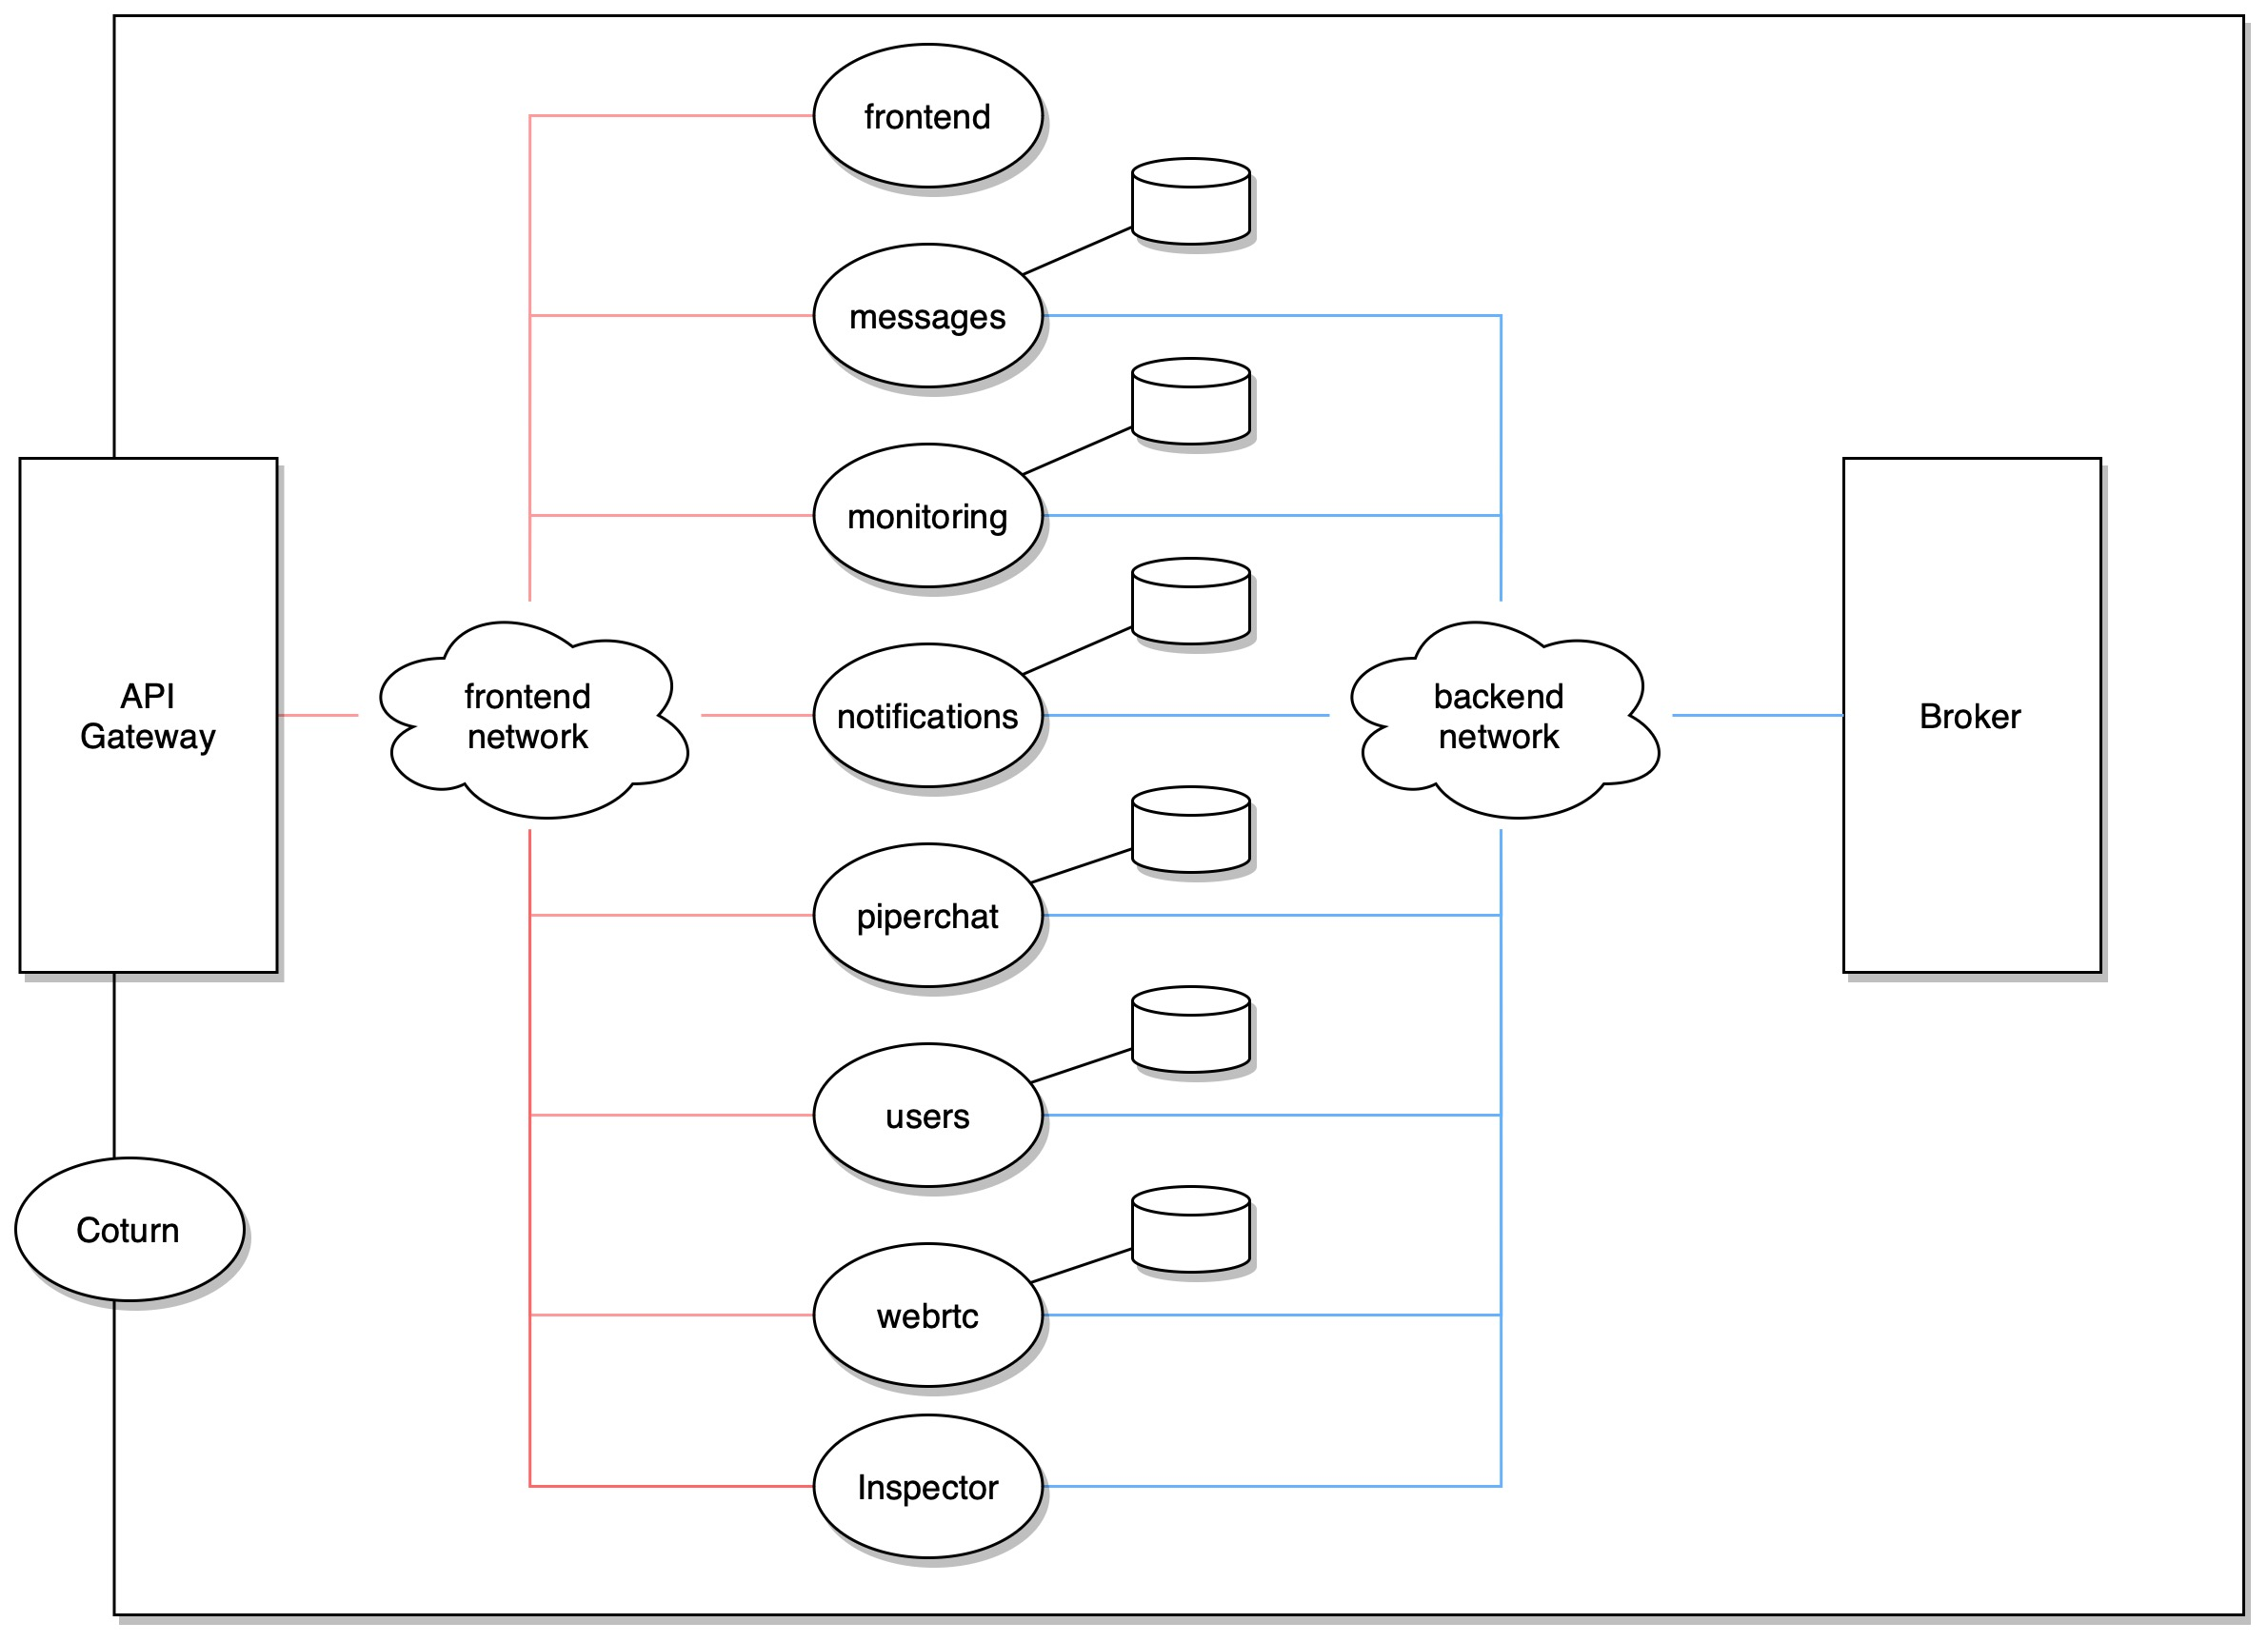
\includegraphics[width=0.85\textwidth]{img/07-deployment/architecture-deployment.jpg}
    \label{fig:architecture-deployment}
\end{figure}

%
%
%
\newpage
\section{Testing deploy}

Per effettuare il testing lato Backend, è stato realizzato un ulteriore \texttt{Docker Compose} il quale ci ha permesso deployare un infrastruttura "alleggerita", dotata unicamente dei container necessari a testare i singoli microservizi, nonché:

\begin{itemize}
    \item Un'istanza del Broker

    \item Un'istanza del database

    \item Un'istanza di Mongo Express per visualizzare il database
\end{itemize}

Questo \texttt{Docker Compose} è situato nella cartella \texttt{/dev}, insieme allo script che ne automatizza l'esecuzione, chiamato \texttt{runDev.sh}.

Di seguito riportato il \texttt{Docker Compose} dell'infrastruttura usata per il testing:

\begin{verbatim}
services:
  db-service:
    image: mongo
    ports:
      - '27017:27017'
    healthcheck:
      test: |
        host=`hostname --ip-address || echo '127.0.0.1'`;
        mongo --quiet $${host}/test --eval
            'quit(db.runCommand({ ping: 1 }).ok ? 0 : 2)' && echo 0 || echo 1

  broker:
    image: rabbitmq:3-management-alpine
    ports:
      - '5672:5672'
      - '15672:15672'
    healthcheck:
      test: ['CMD', 'rabbitmq-diagnostics', '-q', 'ping']

  mongo-express:
    image: mongo-express:latest
    restart: always
    ports:
      - '8081:8081'
    environment:
      ME_CONFIG_MONGODB_SERVER: 'db-service'
    depends_on:
      db-service:
        condition: service_healthy

\end{verbatim}

\section{Esempi d'utilizzo}
Di seguito vengono riportati alcuni esempi di utilizzo della nostra applicazione:

%
%
%
\subsection{Login/Registrazione}
L'accesso a questa sezione non richiede alcuna autenticazione preliminare. Gli utenti hanno la possibilità di effettuare la registrazione o il login per accedere alle funzionalità offerte.

\begin{figure}[htbp]
    \centering
    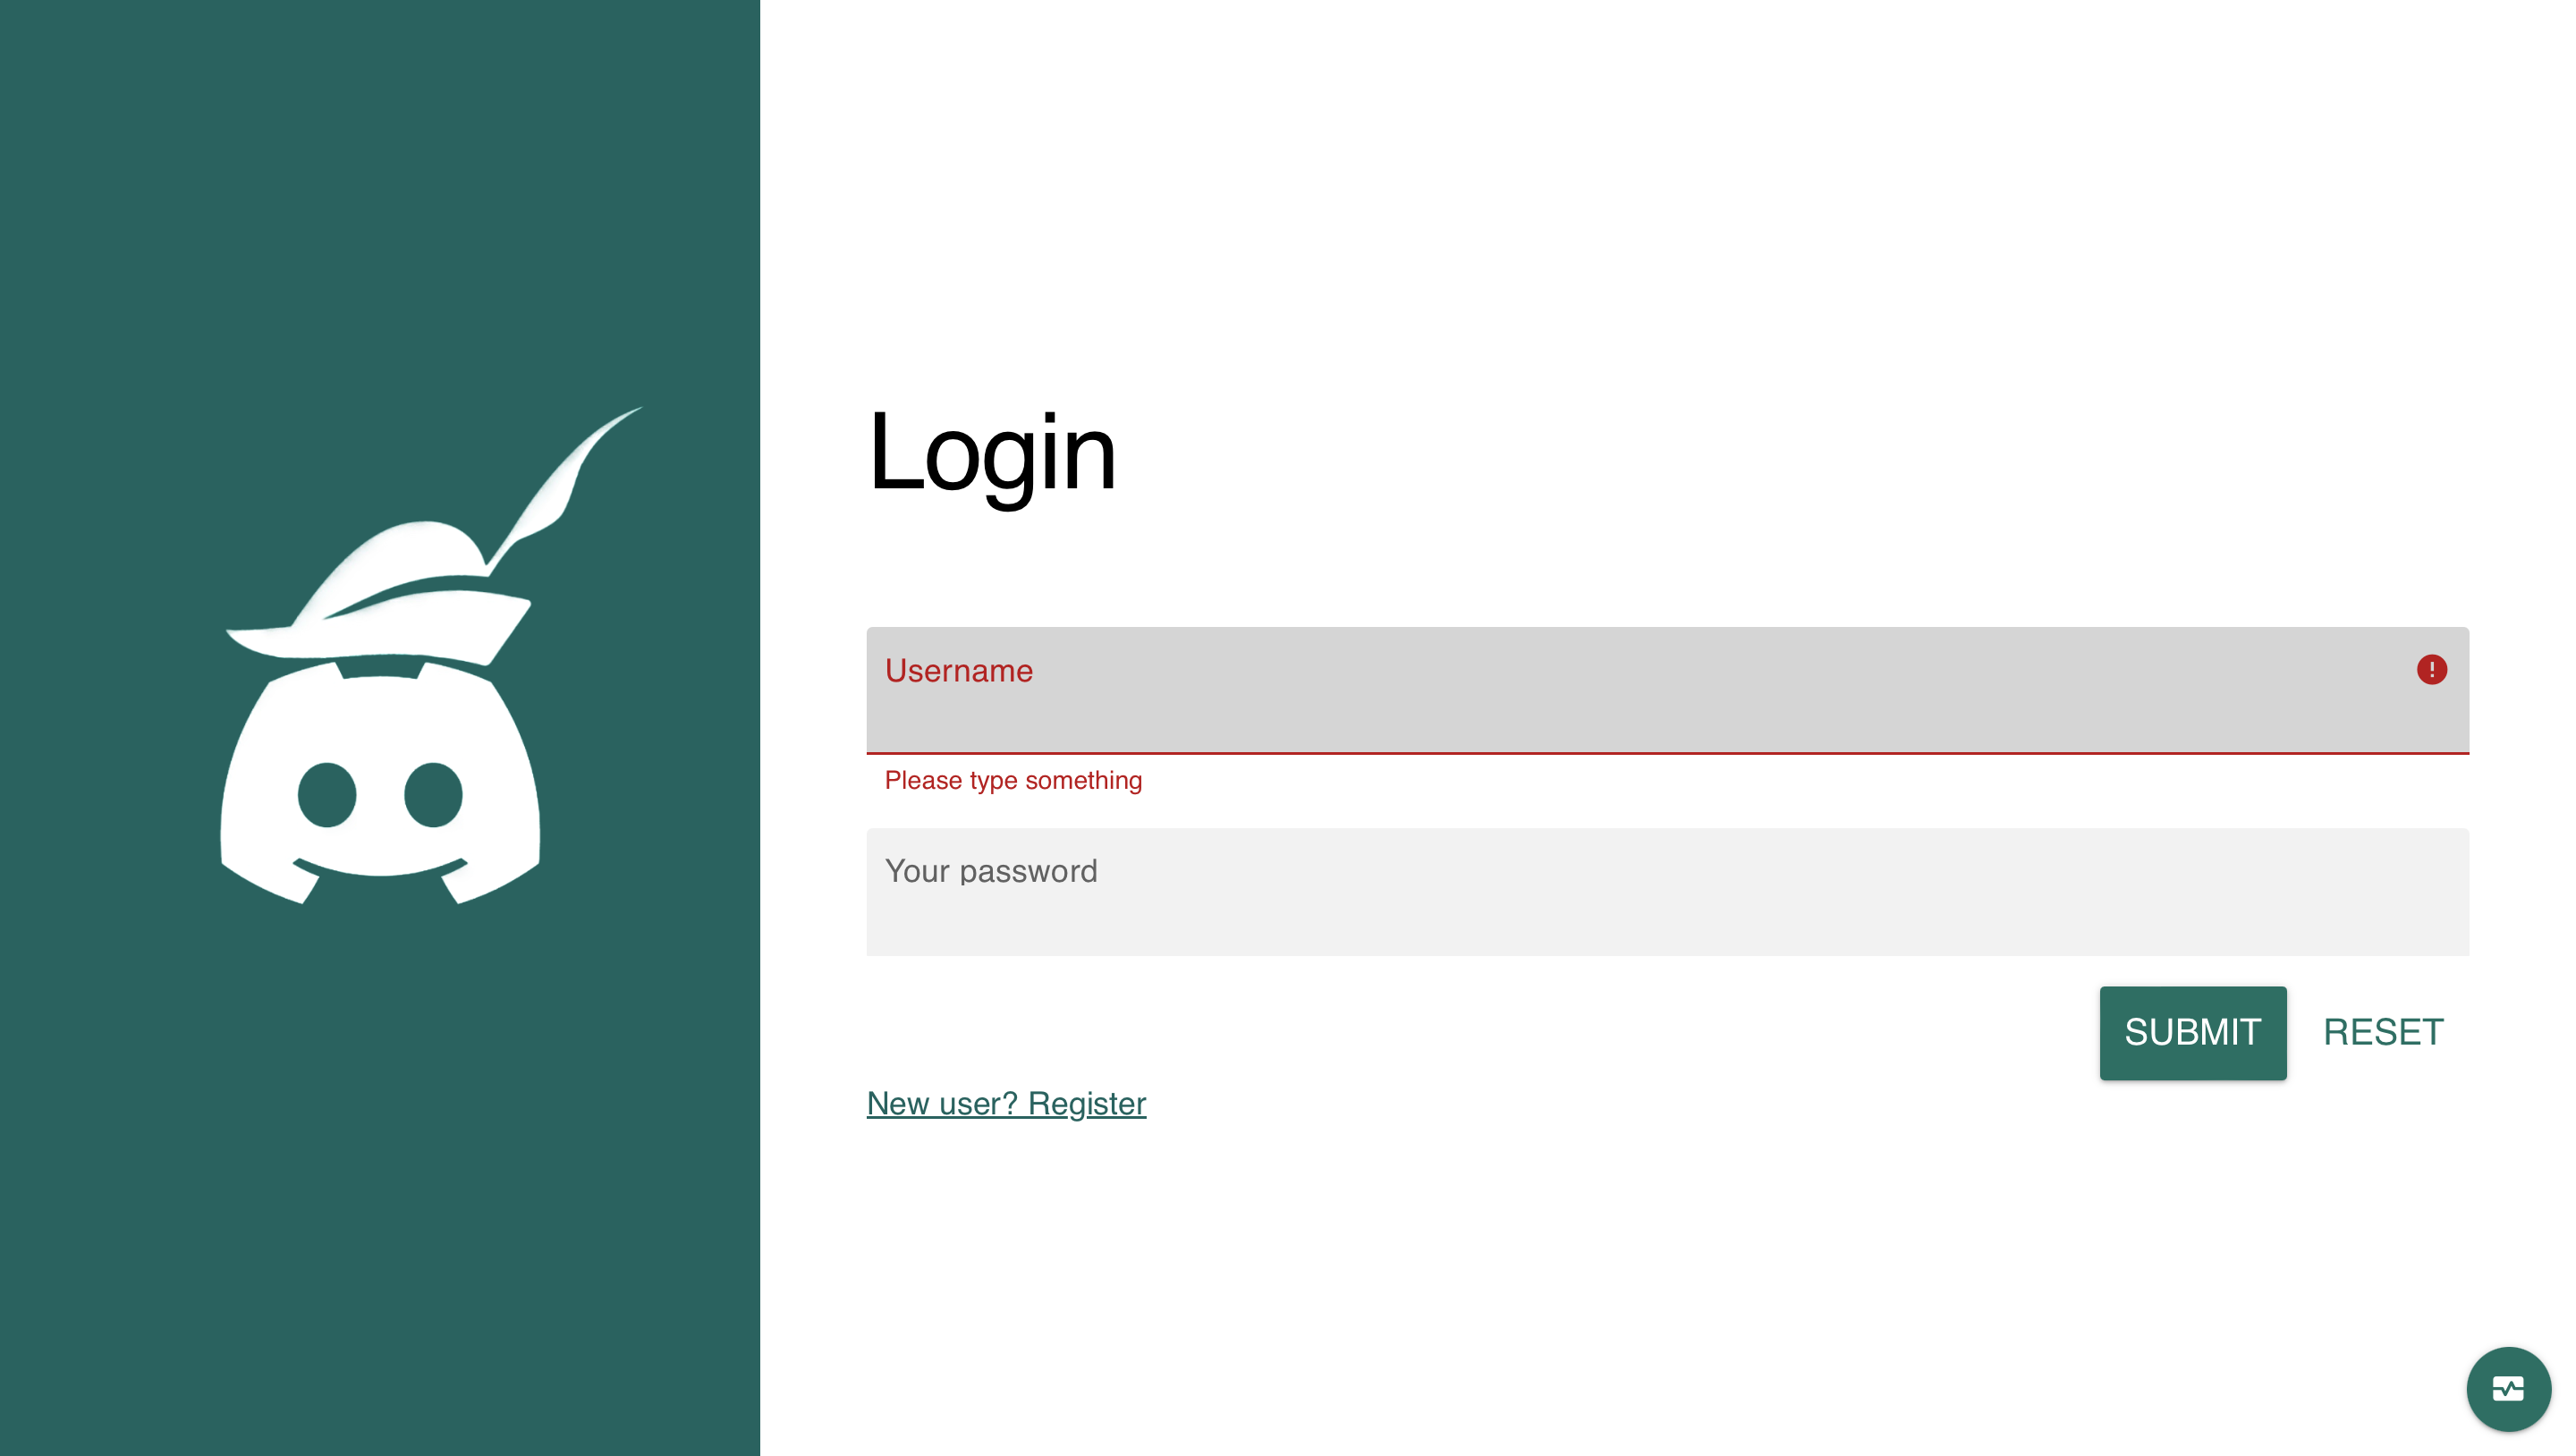
\includegraphics[width=0.9\textwidth]{sections/07-usage-example/img/Login.png}
    \label{fig:login_img}
\end{figure}


\begin{figure}[htbp]
    \centering
    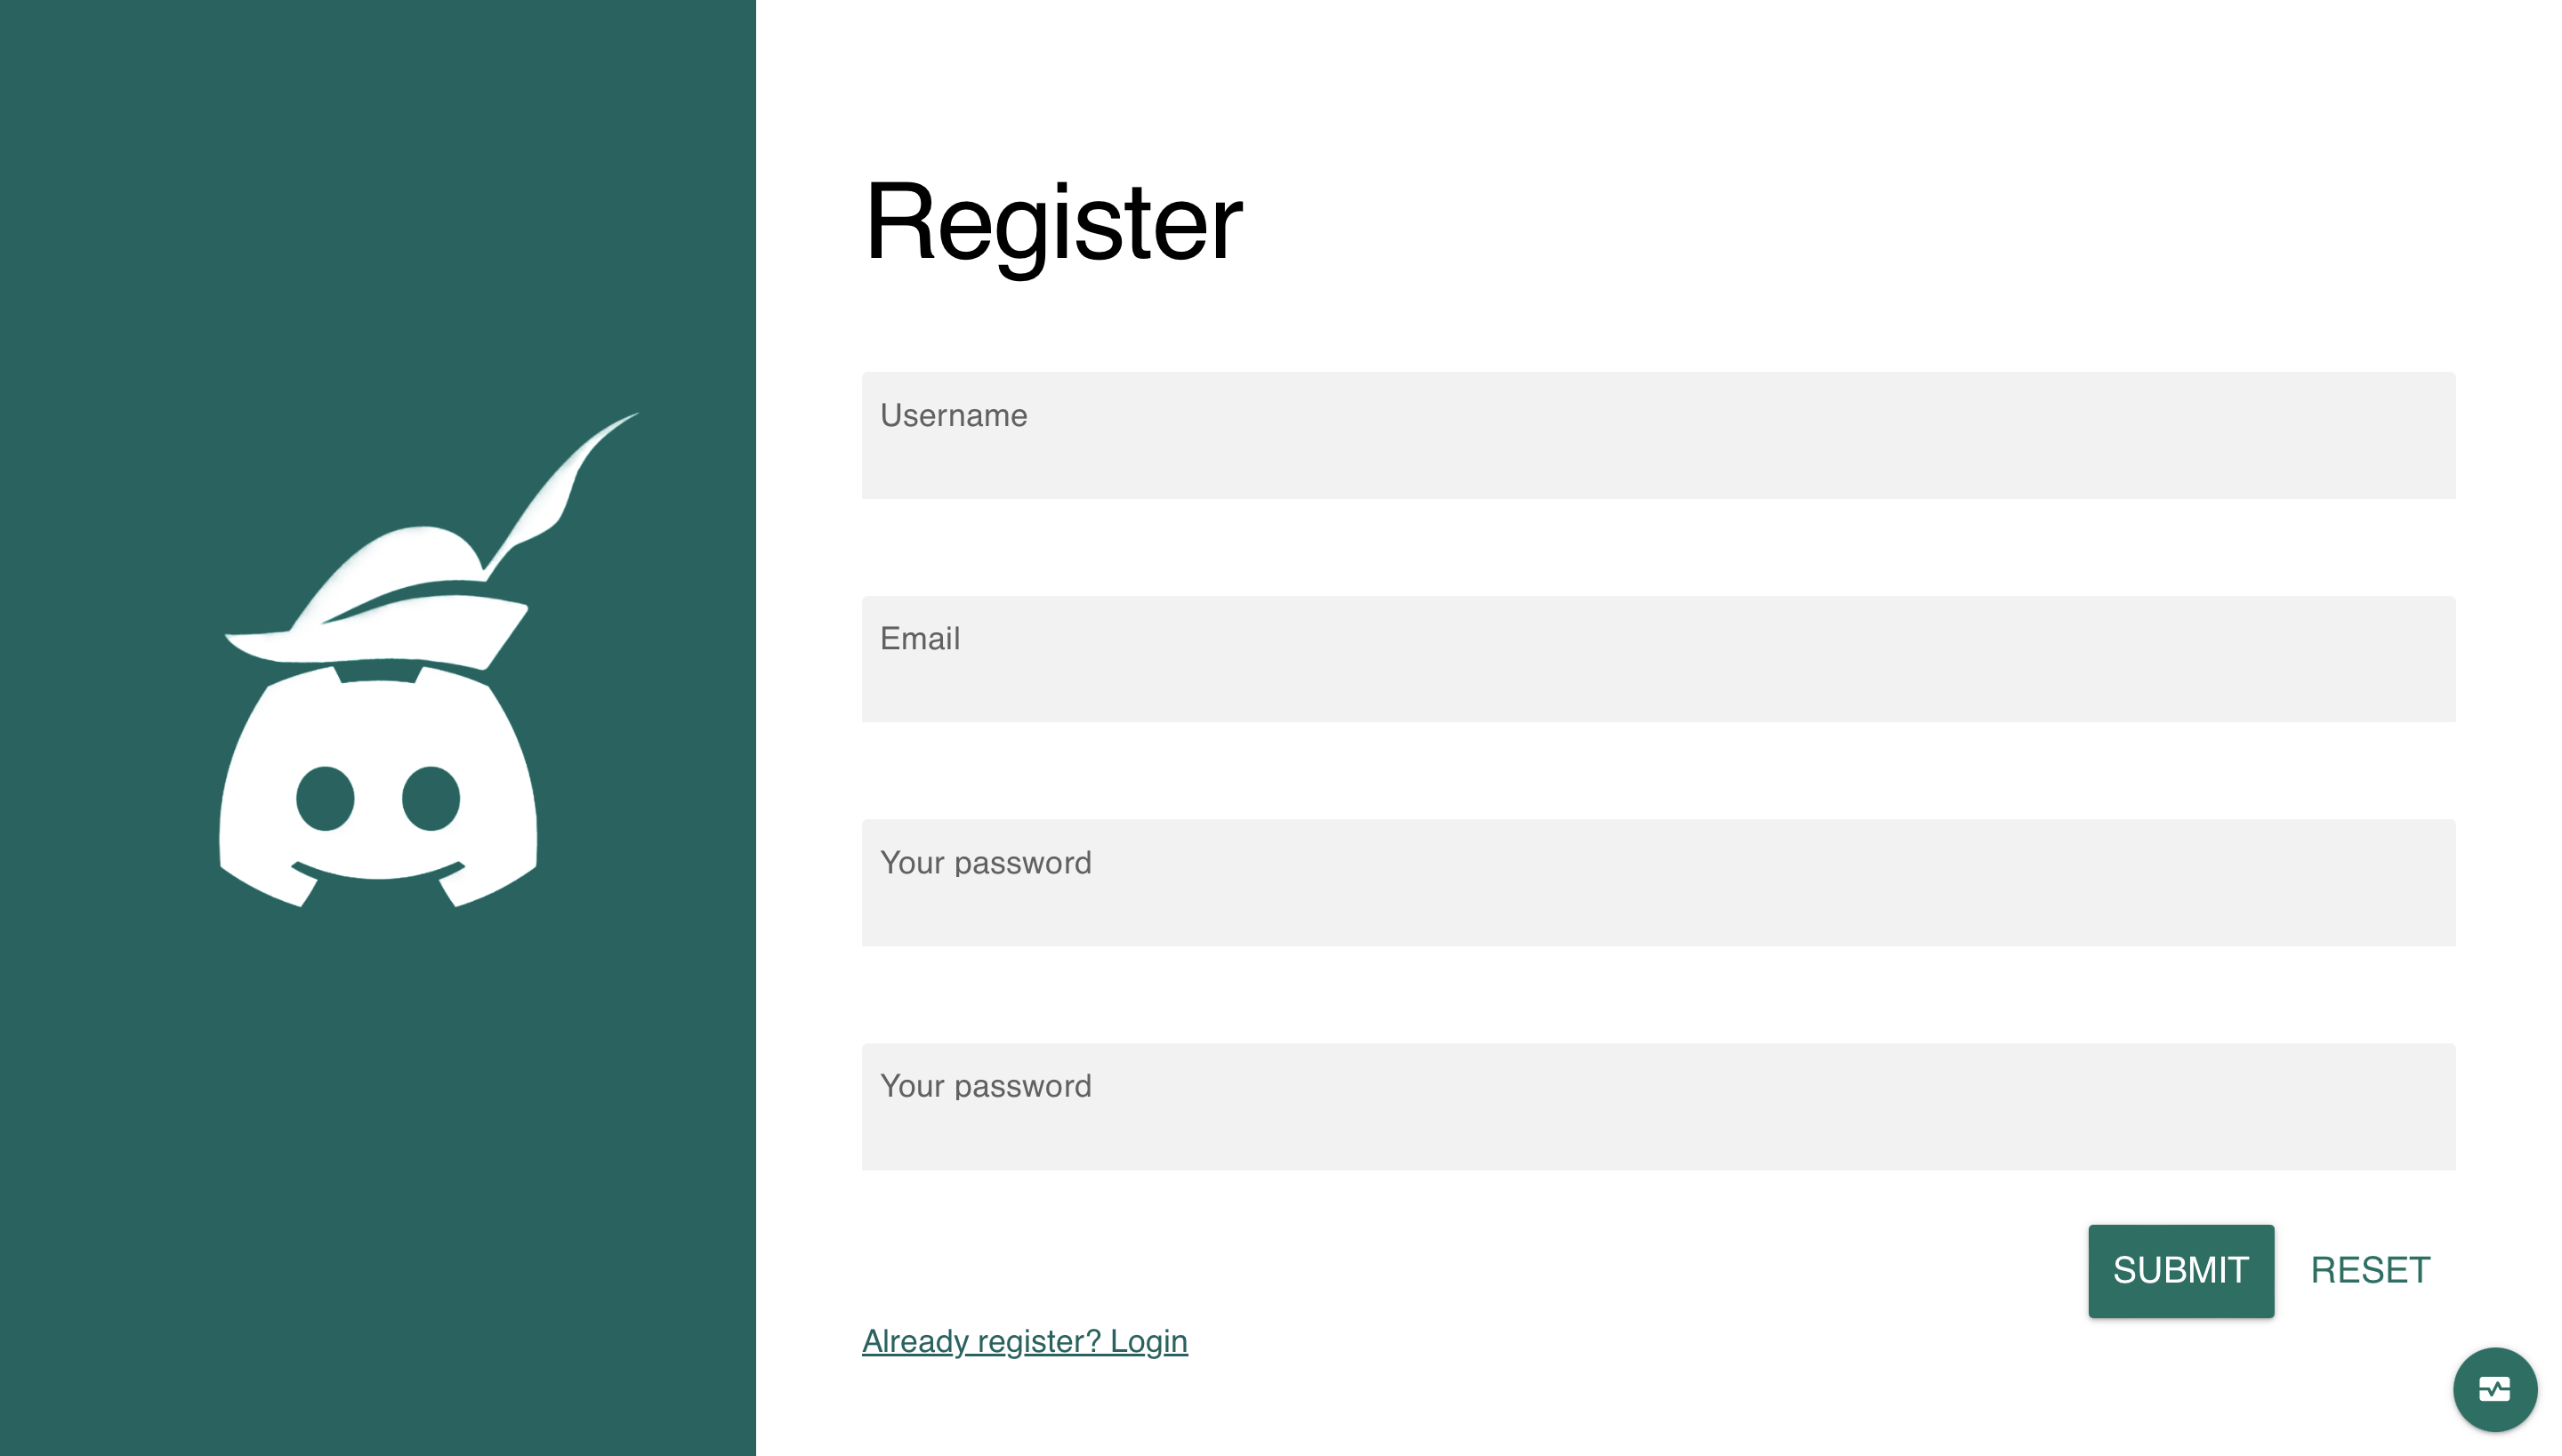
\includegraphics[width=0.9\textwidth]{sections/07-usage-example/img/Register.png}
    \label{fig:register_demo}
\end{figure}

%
%
%
\subsection{Monitoring/Healthcheck}
L'accesso a questa sezione è libero e non richiede credenziali di accesso. Qui gli utenti possono monitorare lo stato dei microservizi in modo rapido e semplice.

\begin{figure}[htbp]
    \centering
    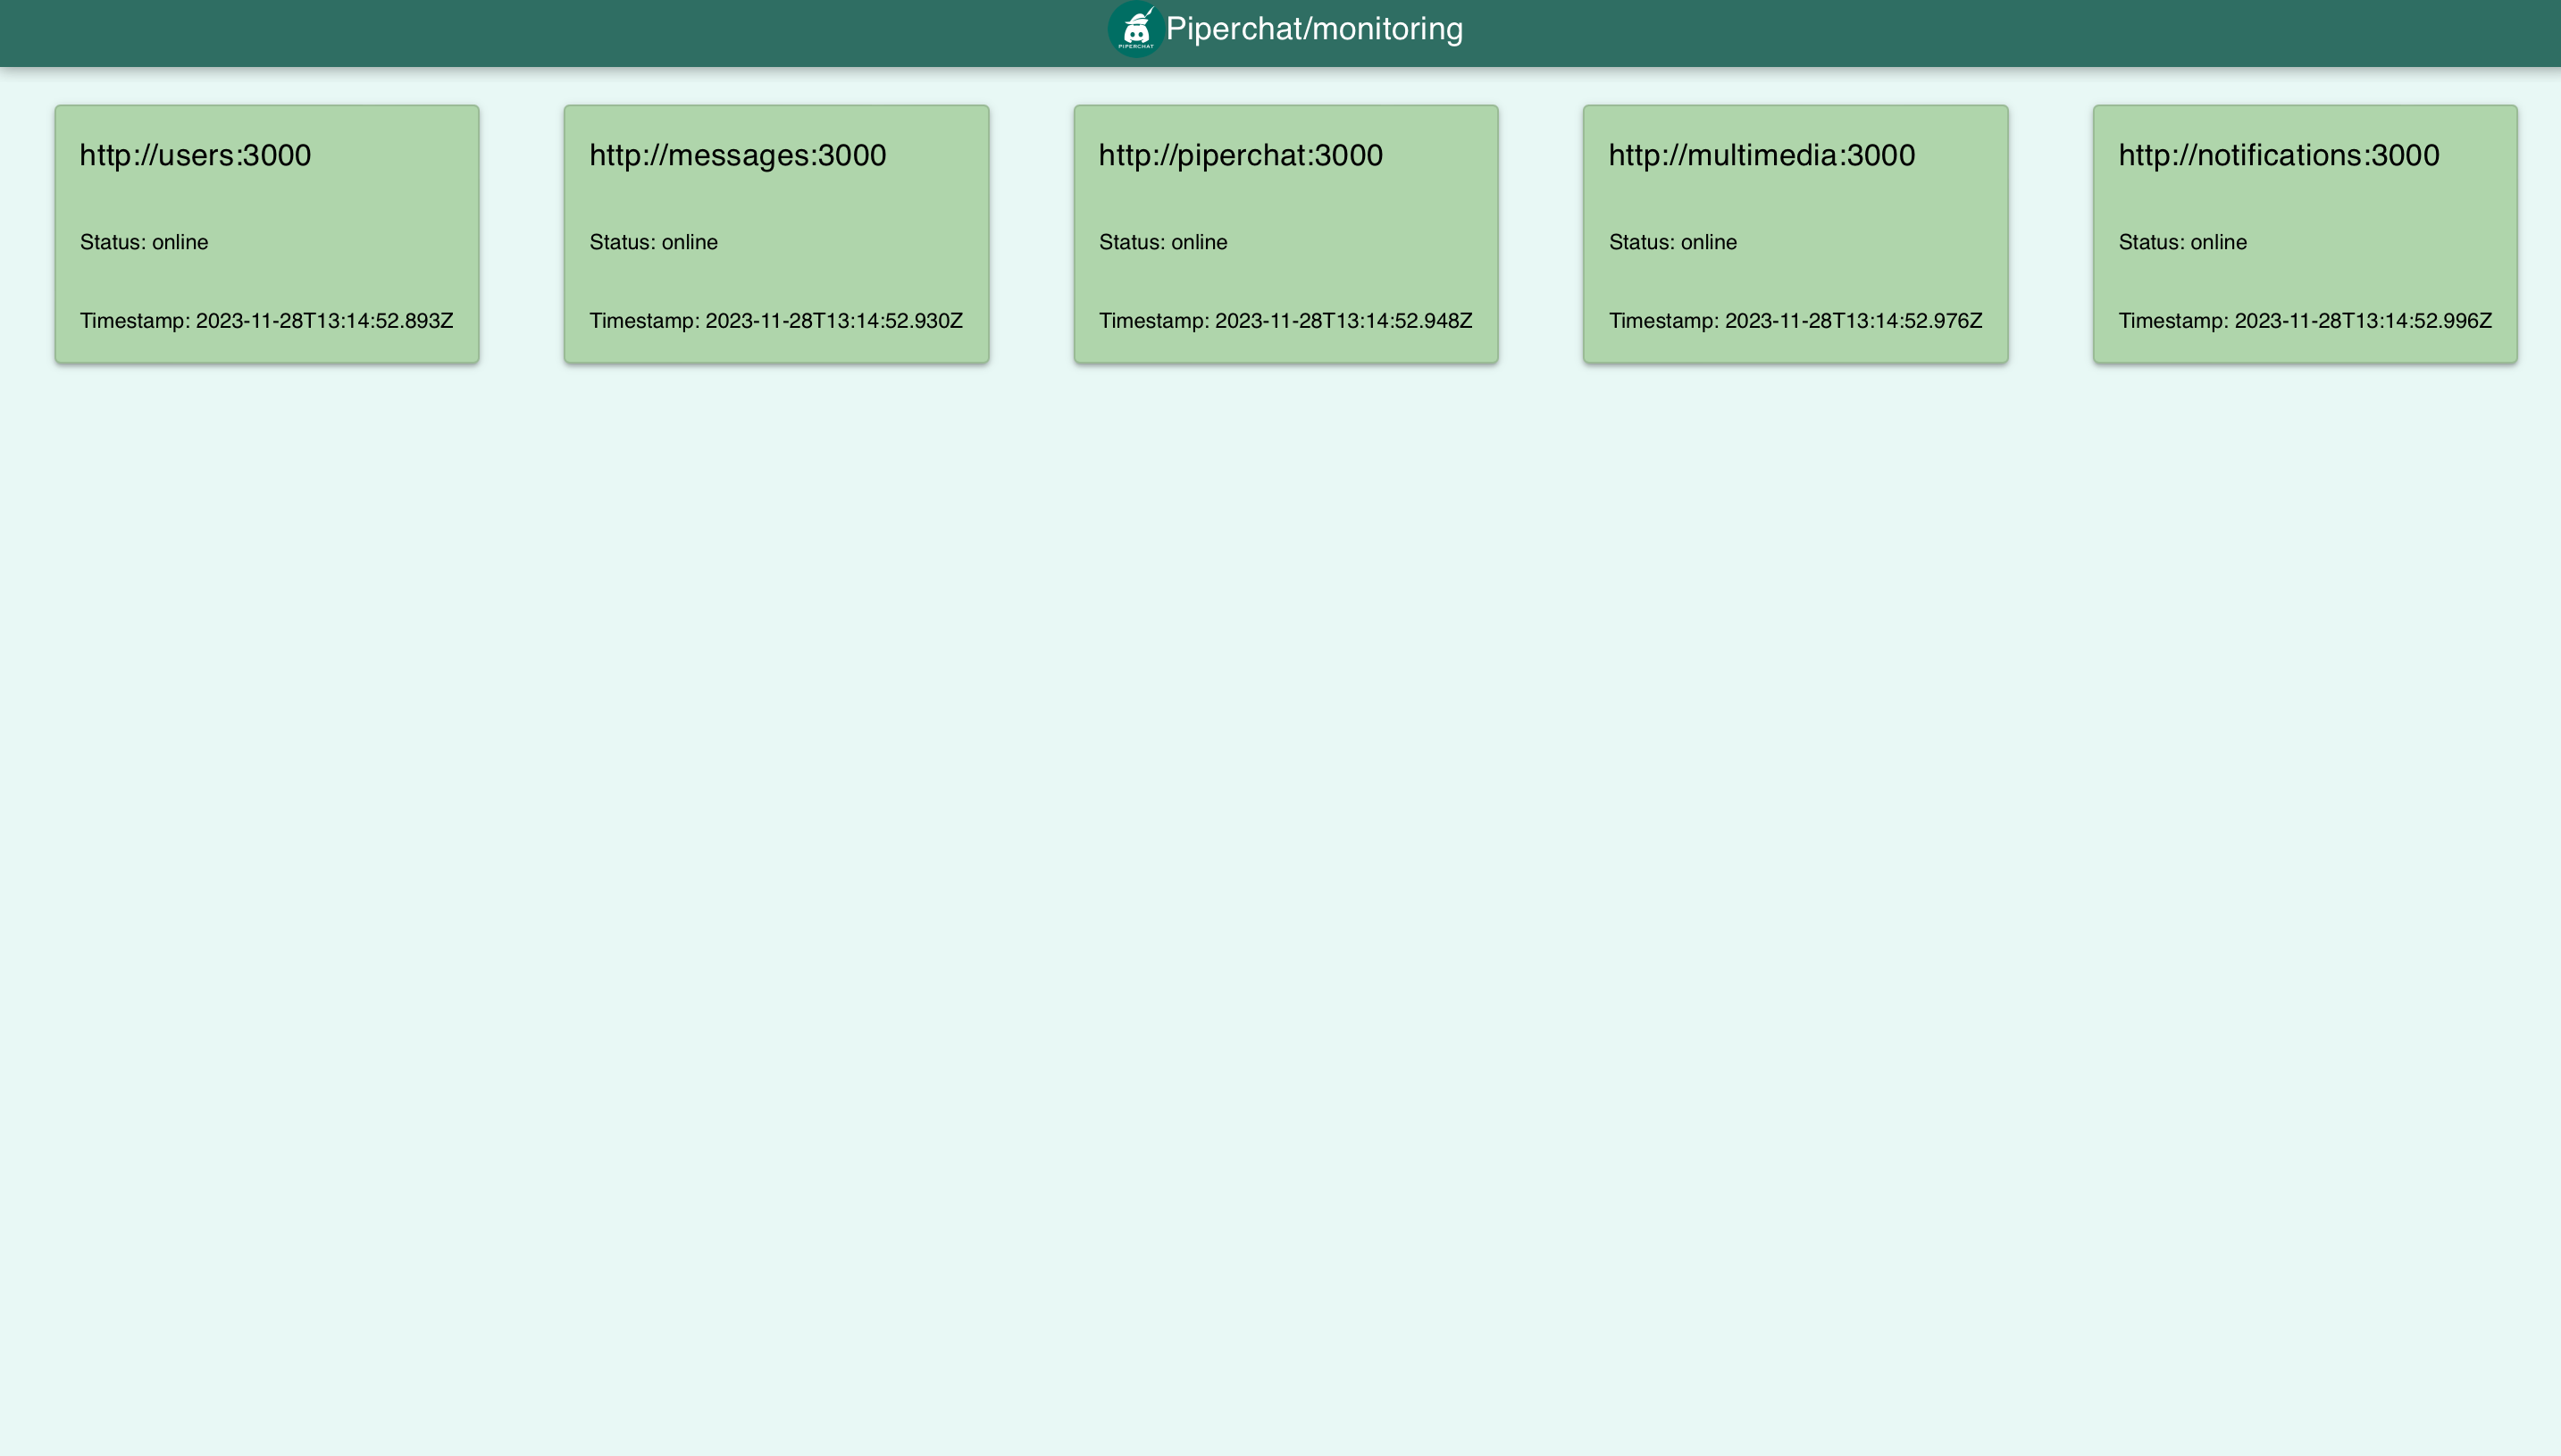
\includegraphics[width=\textwidth]{sections/07-usage-example/img/monitoring.png}
    \label{fig:moitoring_demo}
\end{figure}

%
%
%
\newpage
\subsection{HomePage}
Per accedere a questa sezione è necessario eseguire l'accesso. In caso di assenza di un access token valido, verrà automaticamente reindirizzati alla pagina di login. La struttura della pagina è articolata in due sezioni principali:
\begin{itemize}
    \item \textbf{Menù laterale}: Da qui è possibile navigare tra server, canali e messaggi diretti.
    \item \textbf{Area principale}: Questa sezione mostra i contenuti delle chat e delle videochiamate.
\end{itemize}

\begin{figure}[htbp]
    \centering
    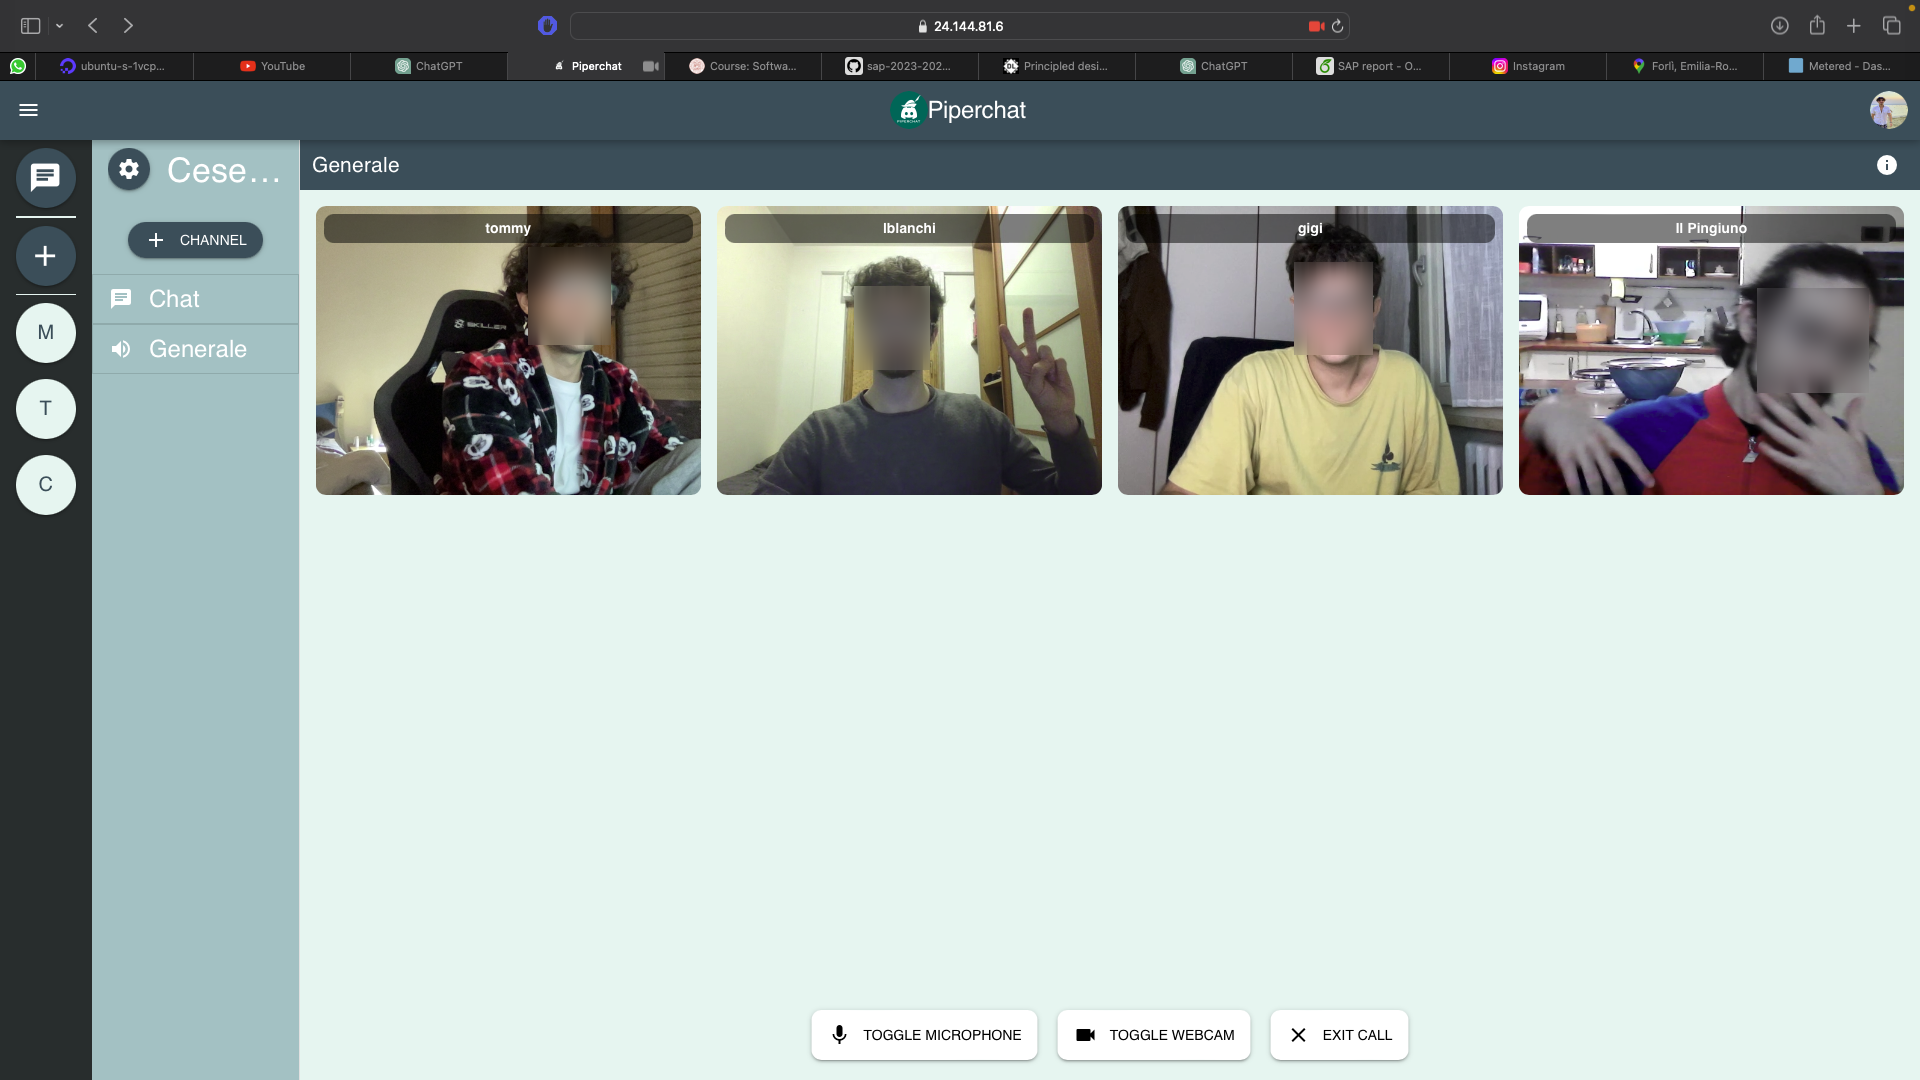
\includegraphics[width=\textwidth]{sections/07-usage-example/img/demo.png}
    \label{fig:webrtc_demo}
\end{figure}

\section{Conclusioni}

Il progetto Piperchat è stato sviluppato con l'obiettivo di creare una piattaforma di comunicazione ispirata a Discord, offrendo agli utenti la possibilità di interagire in varie forme, creare connessioni sociali e gestire server personalizzati. L'architettura a microservizi è stata scelta per gestire la complessità del sistema, consentendo una maggiore coesione e scalabilità.

Durante lo sviluppo, sono stati affrontati diversi aspetti, tra cui la gestione delle amicizie, la messaggistica, la creazione e gestione di server e canali multimediali. L'implementazione di funzionalità come notifiche, chiamate vocali e video ha arricchito l'esperienza dell'utente.

La valutazione della qualità del software prodotto ha considerato aspetti cruciali come funzionalità, affidabilità, scalabilità, sicurezza, usabilità e prestazioni. L'approccio a microservizi ha dimostrato la sua efficacia nel garantire una struttura modulare e gestibile.

\subsection{Sviluppi futuri}
A causa delle scarse tempistiche, l'implementazione della dashboard relativa ai log dell'intera applicazione, è stata messa in secondo piano.
Detto ciò dunque, la prima feature da realizzare in termini di sviluppi futuri sarebbe proprio quest'ultima.

Altro miglioramento che potremmo apportare alla nostra applicazione, riguarderebbe il deploy dell'architettura, difatti attualmente, l'applicazione di videochat viene distribuita utilizzando Docker Compose con un approccio basato su una singola macchina. Tuttavia, per migliorare la scalabilità, la resilienza e la gestione delle risorse, è previsto un futuro passaggio a un'architettura basata su Docker Swarm.


\subsection{Cosa abbiamo imparato}

Durante lo sviluppo di Piperchat, abbiamo acquisito una comprensione approfondita dell'architettura a microservizi e delle sfide associate. Abbiamo imparato a bilanciare aspetti cruciali come la sicurezza, la scalabilità e l'usabilità in un progetto di comunicazione in tempo reale.

La collaborazione tra diversi team per lo sviluppo dei singoli microservizi e la gestione di comunicazione tra di essi attraverso un message broker hanno ampliato la nostra conoscenza delle best practice nello sviluppo di sistemi distribuiti.

Inoltre, l'importanza di valutare la qualità del software in termini di funzionalità, affidabilità e prestazioni ci ha fornito un quadro completo delle sfide e delle opportunità nell'implementazione di una piattaforma di comunicazione complessa come Piperchat.
% \section*{Stylistic Notes}

Use a uniform style, especially when writing formal stuff: $X$, X, $\mathbf{X}$, $\mathcal{X}$, \texttt{X} are all different symbols possibly referring to different entities. 

This is a very short paragraph.

This is a longer paragraph (notice the blank line in the code).
It composed by several sentences.
%
You're invited to use comments within \texttt{.tex} source files to separate sentences composing the same paragraph.

Paragraph should be logically atomic: a subordinate sentence from one paragraph should always refer to another sentence from within the same paragraph.

The first line of a paragraph is usually indented.
%
This is intended: it is the way \LaTeX{} lets the reader know a new paragraph is beginning.

Use the \href{https://en.wikibooks.org/wiki/LaTeX/Source_Code_Listings}{\texttt{listing}} package for inserting scripts into the \LaTeX{} source.

\appendix

\section{Benchmarking}

Di seguito sono riportate le prove di \emph{benchmarking} effettuate, al fine di mettere sotto sforzo il sistema per verificare che la \emph{scalabilità orizzontale} porti parte dei risultati attesi: aumentare il numero di richieste gestite nell'arco di un determinato periodo.

\textbf{Obiettivo:}
il test consiste nell'eseguire lo stesso carico di lavoro lato client variando il numero di repliche del servizio che le deve gestire.

Lo scenario prevede un client che effettua richieste HTTP verso il server, dove è in esecuzione il software di Piperchat, all'interno degli appositi container docker.

%
%
%
\subsection{Configurazione}

Sono state utilizzate le seguenti macchine:

\begin{table}[H]
\centering
\begin{tabular}{|c|cc|}
\hline
\textbf{Componente} & \multicolumn{1}{c|}{\textbf{Client}} & \textbf{Server}           \\ \hline
S.O.                & \multicolumn{1}{c|}{MacOS 14.1}      & Ubuntu 23.10              \\ \hline
CPU                 & \multicolumn{1}{c|}{Apple M1 Pro}    & Intel Core i7-8700 6 core \\ \hline
RAM                 & \multicolumn{1}{c|}{16 GB}           & 16 GB                     \\ \hline
Connessione         & \multicolumn{2}{c|}{Connessione LAN @ $\sim$500 Mbit/s}                \\ \hline
\end{tabular}
\end{table}

Lo strumento utilizzato per effettuare le richieste HTTP lato client è \href{https://github.com/wg/wrk}{\emph{wrk}}, un software di benchmarking che permette di generare carichi di lavoro significativi, sfruttando una singola CPU multi-core.

Il microservizio sotto osservazione è \emph{users-service}, del quale è stata testata la rotta \texttt{/auth/login} con le credenziali di un utente già registrato, attraverso la seguente configurazione:

\begin{verbatim}
$ wrk -t10 -c150 -d30s http://<server-ip>/auth/login -s ./post.lua

// Configurazione script del software (post.lua)
wrk.method = "POST"
wrk.body = '{"username": "user", "password": "12341234"}'
wrk.headers["Content-Type"] = "application/json"
\end{verbatim}

\begin{itemize}
    \item \texttt{-t10:} Vengono impiegati 10 threads
    \item \texttt{-c150:} Vengono simulate 150 connessioni attive (utenti)
    \item \texttt{-d30s:} Il test dura 30 secondi
\end{itemize}

%
%
%
\subsection{Il test}

Il test è stato eseguito più volte, mediante la configurazione esposta in precedenza, variando il numero di repliche del servizio.

Di seguito vengono riportati i risultati, ognuno dei quali è la media di 4 esecuzioni.

\begin{table}[H]
\centering
\caption{1 Replica}
\begin{tabular}{|c|c|ccc}
\hline
\textbf{Thread Stats}   & \textbf{Avg} & \multicolumn{1}{c|}{\textbf{Stdev}} & \multicolumn{1}{l|}{\textbf{Max}} & \multicolumn{1}{l|}{\textbf{+/- Stdev}} \\ \hline
\textbf{Latency}        & 122.43ms     & \multicolumn{1}{c|}{87.88ms}        & \multicolumn{1}{c|}{1.99s}        & \multicolumn{1}{c|}{98.19\%}            \\ \hline
\textbf{Req/Sec}        & 125.04       & \multicolumn{1}{c|}{27.36}          & \multicolumn{1}{c|}{290.00}       & \multicolumn{1}{c|}{84.05\%}            \\ \hline
\textbf{Requests}       & 37424        &                                     &                                   &                                         \\ \cline{1-2}
\textbf{Data Read}      & 9.17MB       &                                     &                                   &                                         \\ \cline{1-2}
\textbf{Socket Timeout} & 49           &                                     &                                   &                                         \\ \cline{1-2}
\end{tabular}
\end{table}
\begin{table}[H]
\caption{2 Repliche}
\centering
\begin{tabular}{|c|c|ccc}
\hline
\textbf{Thread Stats}   & \textbf{Avg} & \multicolumn{1}{c|}{\textbf{Stdev}} & \multicolumn{1}{l|}{\textbf{Max}} & \multicolumn{1}{l|}{\textbf{+/- Stdev}} \\ \hline
\textbf{Latency}        & 88.17ms      & \multicolumn{1}{c|}{113.72ms}       & \multicolumn{1}{c|}{1.84s}        & \multicolumn{1}{c|}{97.79\%}            \\ \hline
\textbf{Req/Sec}        & 202.99       & \multicolumn{1}{c|}{35.28}          & \multicolumn{1}{c|}{350.00}       & \multicolumn{1}{c|}{70.80\%}            \\ \hline
\textbf{Requests}       & 60708        &                                     &                                   &                                         \\ \cline{1-2}
\textbf{Data Read}      & 14.88MB      &                                     &                                   &                                         \\ \cline{1-2}
\textbf{Socket Timeout} & 20           &                                     &                                   &                                         \\ \cline{1-2}
\end{tabular}
\end{table}
\begin{table}[H]
\caption{3 Repliche}
\centering
\begin{tabular}{|c|c|ccc}
\hline
\textbf{Thread Stats}   & \textbf{Avg} & \multicolumn{1}{c|}{\textbf{Stdev}} & \multicolumn{1}{l|}{\textbf{Max}} & \multicolumn{1}{l|}{\textbf{+/- Stdev}} \\ \hline
\textbf{Latency}        & 71.24ms      & \multicolumn{1}{c|}{108.48ms}       & \multicolumn{1}{c|}{1.87s}        & \multicolumn{1}{c|}{96.68\%}            \\ \hline
\textbf{Req/Sec}        & 255.34       & \multicolumn{1}{c|}{45.02}          & \multicolumn{1}{c|}{460.00}       & \multicolumn{1}{c|}{71.90\%}            \\ \hline
\textbf{Requests}       & 76351        &                                     &                                   &                                         \\ \cline{1-2}
\textbf{Data Read}      & 18.71MB      &                                     &                                   &                                         \\ \cline{1-2}
\textbf{Socket Timeout} & 10           &                                     &                                   &                                         \\ \cline{1-2}
\end{tabular}
\end{table}
\begin{table}[H]
\caption{5 Repliche}
\centering
\begin{tabular}{|c|c|ccc}
\hline
\textbf{Thread Stats}   & \textbf{Avg} & \multicolumn{1}{c|}{\textbf{Stdev}} & \multicolumn{1}{l|}{\textbf{Max}} & \multicolumn{1}{l|}{\textbf{+/- Stdev}} \\ \hline
\textbf{Latency}        & 61.14ms      & \multicolumn{1}{c|}{113.39ms}       & \multicolumn{1}{c|}{1.87s}        & \multicolumn{1}{c|}{96.97\%}            \\ \hline
\textbf{Req/Sec}        & 332.08       & \multicolumn{1}{c|}{56.51}          & \multicolumn{1}{c|}{560.00}       & \multicolumn{1}{c|}{74.39\%}            \\ \hline
\textbf{Requests}       & 100839       &                                     &                                   &                                         \\ \cline{1-2}
\textbf{Data Read}      & 24.28MB      &                                     &                                   &                                         \\ \cline{1-2}
\textbf{Socket Timeout} & 6            &                                     &                                   &                                         \\ \cline{1-2}
\end{tabular}
\end{table}
\begin{table}[H]
\caption{10 Repliche}
\centering
\begin{tabular}{|c|c|ccc}
\hline
\textbf{Thread Stats}   & \textbf{Avg} & \multicolumn{1}{c|}{\textbf{Stdev}} & \multicolumn{1}{l|}{\textbf{Max}} & \multicolumn{1}{l|}{\textbf{+/- Stdev}} \\ \hline
\textbf{Latency}        & 43.87ms      & \multicolumn{1}{c|}{29.17ms}        & \multicolumn{1}{c|}{413.79ms}     & \multicolumn{1}{c|}{88.57\%}            \\ \hline
\textbf{Req/Sec}        & 370.84       & \multicolumn{1}{c|}{74.67}          & \multicolumn{1}{c|}{545.00}       & \multicolumn{1}{c|}{80.13\%}            \\ \hline
\textbf{Requests}       & 110072       &                                     &                                   &                                         \\ \cline{1-2}
\textbf{Data Read}      & 26.98MB      &                                     &                                   &                                         \\ \cline{1-2}
\textbf{Socket Timeout} & 0            &                                     &                                   &                                         \\ \cline{1-2}
\end{tabular}
\end{table}
\begin{table}[H]
\caption{20 Repliche}
\centering
\label{tab:bench-replica-20}
\begin{tabular}{|c|c|ccc}
\hline
\textbf{Thread Stats}   & \textbf{Avg} & \multicolumn{1}{c|}{\textbf{Stdev}} & \multicolumn{1}{l|}{\textbf{Max}} & \multicolumn{1}{l|}{\textbf{+/- Stdev}} \\ \hline
\textbf{Latency}        & 137.94ms     & \multicolumn{1}{c|}{213.60ms}       & \multicolumn{1}{c|}{1.98s}        & \multicolumn{1}{c|}{91.61\%}            \\ \hline
\textbf{Req/Sec}        & 162.18       & \multicolumn{1}{c|}{108.81}         & \multicolumn{1}{c|}{420.00}       & \multicolumn{1}{c|}{58.31\%}            \\ \hline
\textbf{Requests}       & 15308        &                                     &                                   &                                         \\ \cline{1-2}
\textbf{Data Read}      & 3.52MB       &                                     &                                   &                                         \\ \cline{1-2}
\textbf{Socket Timeout} & 550          &                                     &                                   &                                         \\ \cline{1-2}
\end{tabular}
\end{table}

%
%
%
\subsection{Risultati}

Il test effettuato ha portato ai risultati attesi.
%
I dati di maggior rilievo da prendere che possono essere osservati sono la \emph{latenza} ed il \emph{numero di richieste}.

Come si può notare, il numero di richieste tendere ad aumentare finché non si arriva al numero di repliche uguale al numero di core effettivi della macchina che deve prendere in carico la richiesta, per poi stabilizzarsi.

Invece, la latenza di risposta alle richieste tende a diminuire costantemente finché non si raggiunge il numero di threads\footnote{Intel® Hyper-Threading Technology} di cui dispone la macchina.

Superati i numeri evidenziati in precedenza, le prestazioni iniziano a degradare.
%
Come si può notare in Tabella \ref{tab:bench-replica-20}, il numero di socket che non riesce ad effettuare una connessione tende ad aumentare notevolmente.
\section{Tentativo di deployment reale}

Abbiamo proceduto con il deploy dell'applicazione online con l'obiettivo di testare e utilizzare concretamente l'applicativo. Durante questo processo, sono emersi alcuni problemi rilevanti relativi all'implementazione delle WebSocket.

\subsection{Problema con WebSocket non Sicure}
Durante il deploy, ci siamo accorti che l'applicazione utilizzava WebSocket non sicure (ws) invece di WebSocket sicure (wss). Questo ha causato il blocco delle connessioni da parte dei browser, poiché molti moderni browser richiedono connessioni sicure per proteggere la privacy degli utenti.

Per affrontare questo problema, abbiamo implementato una soluzione intermedia utilizzando Nginx come proxy SSL. Nginx è stato configurato per gestire la crittografia SSL/TLS delle connessioni WebSocket, consentendo l'utilizzo di connessioni sicure (wss). Questo approccio ci ha permesso di ottenere connessioni sicure senza dover apportare modifiche dirette al codice sorgente dell'applicazione. 

\begin{verbatim}
location / {
    # Configurazione del proxy pass verso il server sulla porta 80
    proxy_pass http://localhost:80;
    proxy_set_header Host $host;
    proxy_set_header X-Real-IP $remote_addr;
    proxy_set_header X-Forwarded-For $proxy_add_x_forwarded_for;
    proxy_set_header X-Forwarded-Proto $scheme;
}

location /notification {
    proxy_pass http://localhost:80;
    proxy_http_version 1.1;
    proxy_set_header Upgrade $http_upgrade;
    proxy_set_header Connection "upgrade";
}

location /webrtc {
    proxy_pass http://localhost:80;
    proxy_http_version 1.1;
    proxy_set_header Upgrade $http_upgrade;
    proxy_set_header Connection "upgrade";
}
\end{verbatim}

\section{Sperimentale: deploy con Dev Containers}

A fini sperimentali, è stato eseguito il deploy dell'infrastruttura attraverso la tecnologia \emph{Dev Containers} di GitHub.

Di seguito sono riportate le istruzioni per eseguire il deploy:

\begin{enumerate}
    \item Fork del repository

    \item Dalla pagina di GitHub
\begin{verbatim}
Code > Codespaces > Create codespace on main
\end{verbatim}

    \item Attendere la creazione dell'ambiente.

    \item Utilizzare il servizio tramite il link fornito dall'ambiente di codespace.

    \item (Opzionale) Modificare la visibilità delle porte tramite l'interfaccia grafica nell'apposita sezione, in modo da permettere di utilizzare il sistema anche a terzi, tramite il link fornito.
\end{enumerate}


% \nocite{*} % Includes all references from the `references.bib` file
% \bibliographystyle{plain}
% \bibliography{references}
\end{document}
